% Options for packages loaded elsewhere
\PassOptionsToPackage{unicode}{hyperref}
\PassOptionsToPackage{hyphens}{url}
%
\documentclass[
]{book}
\usepackage{amsmath,amssymb}
\usepackage{iftex}
\ifPDFTeX
  \usepackage[T1]{fontenc}
  \usepackage[utf8]{inputenc}
  \usepackage{textcomp} % provide euro and other symbols
\else % if luatex or xetex
  \usepackage{unicode-math} % this also loads fontspec
  \defaultfontfeatures{Scale=MatchLowercase}
  \defaultfontfeatures[\rmfamily]{Ligatures=TeX,Scale=1}
\fi
\usepackage{lmodern}
\ifPDFTeX\else
  % xetex/luatex font selection
\fi
% Use upquote if available, for straight quotes in verbatim environments
\IfFileExists{upquote.sty}{\usepackage{upquote}}{}
\IfFileExists{microtype.sty}{% use microtype if available
  \usepackage[]{microtype}
  \UseMicrotypeSet[protrusion]{basicmath} % disable protrusion for tt fonts
}{}
\makeatletter
\@ifundefined{KOMAClassName}{% if non-KOMA class
  \IfFileExists{parskip.sty}{%
    \usepackage{parskip}
  }{% else
    \setlength{\parindent}{0pt}
    \setlength{\parskip}{6pt plus 2pt minus 1pt}}
}{% if KOMA class
  \KOMAoptions{parskip=half}}
\makeatother
\usepackage{xcolor}
\usepackage{color}
\usepackage{fancyvrb}
\newcommand{\VerbBar}{|}
\newcommand{\VERB}{\Verb[commandchars=\\\{\}]}
\DefineVerbatimEnvironment{Highlighting}{Verbatim}{commandchars=\\\{\}}
% Add ',fontsize=\small' for more characters per line
\usepackage{framed}
\definecolor{shadecolor}{RGB}{248,248,248}
\newenvironment{Shaded}{\begin{snugshade}}{\end{snugshade}}
\newcommand{\AlertTok}[1]{\textcolor[rgb]{0.94,0.16,0.16}{#1}}
\newcommand{\AnnotationTok}[1]{\textcolor[rgb]{0.56,0.35,0.01}{\textbf{\textit{#1}}}}
\newcommand{\AttributeTok}[1]{\textcolor[rgb]{0.13,0.29,0.53}{#1}}
\newcommand{\BaseNTok}[1]{\textcolor[rgb]{0.00,0.00,0.81}{#1}}
\newcommand{\BuiltInTok}[1]{#1}
\newcommand{\CharTok}[1]{\textcolor[rgb]{0.31,0.60,0.02}{#1}}
\newcommand{\CommentTok}[1]{\textcolor[rgb]{0.56,0.35,0.01}{\textit{#1}}}
\newcommand{\CommentVarTok}[1]{\textcolor[rgb]{0.56,0.35,0.01}{\textbf{\textit{#1}}}}
\newcommand{\ConstantTok}[1]{\textcolor[rgb]{0.56,0.35,0.01}{#1}}
\newcommand{\ControlFlowTok}[1]{\textcolor[rgb]{0.13,0.29,0.53}{\textbf{#1}}}
\newcommand{\DataTypeTok}[1]{\textcolor[rgb]{0.13,0.29,0.53}{#1}}
\newcommand{\DecValTok}[1]{\textcolor[rgb]{0.00,0.00,0.81}{#1}}
\newcommand{\DocumentationTok}[1]{\textcolor[rgb]{0.56,0.35,0.01}{\textbf{\textit{#1}}}}
\newcommand{\ErrorTok}[1]{\textcolor[rgb]{0.64,0.00,0.00}{\textbf{#1}}}
\newcommand{\ExtensionTok}[1]{#1}
\newcommand{\FloatTok}[1]{\textcolor[rgb]{0.00,0.00,0.81}{#1}}
\newcommand{\FunctionTok}[1]{\textcolor[rgb]{0.13,0.29,0.53}{\textbf{#1}}}
\newcommand{\ImportTok}[1]{#1}
\newcommand{\InformationTok}[1]{\textcolor[rgb]{0.56,0.35,0.01}{\textbf{\textit{#1}}}}
\newcommand{\KeywordTok}[1]{\textcolor[rgb]{0.13,0.29,0.53}{\textbf{#1}}}
\newcommand{\NormalTok}[1]{#1}
\newcommand{\OperatorTok}[1]{\textcolor[rgb]{0.81,0.36,0.00}{\textbf{#1}}}
\newcommand{\OtherTok}[1]{\textcolor[rgb]{0.56,0.35,0.01}{#1}}
\newcommand{\PreprocessorTok}[1]{\textcolor[rgb]{0.56,0.35,0.01}{\textit{#1}}}
\newcommand{\RegionMarkerTok}[1]{#1}
\newcommand{\SpecialCharTok}[1]{\textcolor[rgb]{0.81,0.36,0.00}{\textbf{#1}}}
\newcommand{\SpecialStringTok}[1]{\textcolor[rgb]{0.31,0.60,0.02}{#1}}
\newcommand{\StringTok}[1]{\textcolor[rgb]{0.31,0.60,0.02}{#1}}
\newcommand{\VariableTok}[1]{\textcolor[rgb]{0.00,0.00,0.00}{#1}}
\newcommand{\VerbatimStringTok}[1]{\textcolor[rgb]{0.31,0.60,0.02}{#1}}
\newcommand{\WarningTok}[1]{\textcolor[rgb]{0.56,0.35,0.01}{\textbf{\textit{#1}}}}
\usepackage{longtable,booktabs,array}
\usepackage{calc} % for calculating minipage widths
% Correct order of tables after \paragraph or \subparagraph
\usepackage{etoolbox}
\makeatletter
\patchcmd\longtable{\par}{\if@noskipsec\mbox{}\fi\par}{}{}
\makeatother
% Allow footnotes in longtable head/foot
\IfFileExists{footnotehyper.sty}{\usepackage{footnotehyper}}{\usepackage{footnote}}
\makesavenoteenv{longtable}
\usepackage{graphicx}
\makeatletter
\def\maxwidth{\ifdim\Gin@nat@width>\linewidth\linewidth\else\Gin@nat@width\fi}
\def\maxheight{\ifdim\Gin@nat@height>\textheight\textheight\else\Gin@nat@height\fi}
\makeatother
% Scale images if necessary, so that they will not overflow the page
% margins by default, and it is still possible to overwrite the defaults
% using explicit options in \includegraphics[width, height, ...]{}
\setkeys{Gin}{width=\maxwidth,height=\maxheight,keepaspectratio}
% Set default figure placement to htbp
\makeatletter
\def\fps@figure{htbp}
\makeatother
\setlength{\emergencystretch}{3em} % prevent overfull lines
\providecommand{\tightlist}{%
  \setlength{\itemsep}{0pt}\setlength{\parskip}{0pt}}
\setcounter{secnumdepth}{5}
\usepackage{booktabs}
\ifLuaTeX
  \usepackage{selnolig}  % disable illegal ligatures
\fi
\usepackage[]{natbib}
\bibliographystyle{apalike}
\IfFileExists{bookmark.sty}{\usepackage{bookmark}}{\usepackage{hyperref}}
\IfFileExists{xurl.sty}{\usepackage{xurl}}{} % add URL line breaks if available
\urlstyle{same}
\hypersetup{
  pdftitle={Evolución de secuencias palindromicas en genomas de cianobacterias},
  pdfauthor={Eduardo Padilla Mendoza},
  hidelinks,
  pdfcreator={LaTeX via pandoc}}

\title{Evolución de secuencias palindromicas en genomas de cianobacterias}
\author{Eduardo Padilla Mendoza}
\date{2023-08-17}

\begin{document}
\maketitle

{
\setcounter{tocdepth}{1}
\tableofcontents
}
\hypertarget{resumen}{%
\chapter*{Resumen}\label{resumen}}
\addcontentsline{toc}{chapter}{Resumen}

El palíndromo altamente iterado 1 (HIP1 por sus siglas en inglés) cuya secuencia es 5'-GCGATCGC-3', está ampliamente representado en las cianobacterias con excepción de las pico-cianobacterias marinas y otros linajes. El origen de HIP1 y su función (si es que tiene alguna) permanecen desconocidos. Se ha observado que el sitio de reconocimiento (5'-Gm6ATC-3 `) de la enzima Dam metiltransferasa específica para adenina N6 de clase D12 (Dam-met) y el sitio de reconocimiento de DmtC (5'-m5CGATCG-3 ') están contenidos en HIP1, lo que sugiere una posible relación. Sin embargo, la asociación funcional de otros genes con HIP1 no se ha reportado.

\hypertarget{introducciuxf3n}{%
\chapter{Introducción}\label{introducciuxf3n}}

\hypertarget{muxe9todos}{%
\chapter{Métodos}\label{muxe9todos}}

Se descargaron 2 conjuntos de genomas de cianobacterias del servidor del NCBI (\url{https://www.ncbi.nlm.nih.gov/genome/browse/\#!/prokaryotes}).

Estos conjuntos corresponden a:

\begin{itemize}
\tightlist
\item
  269 genomas completos y aquellos que solo contenian el cromosoma (\textbf{complete\_chr})
\item
  165 genomas nuevos usados en \citet{cabello2022elucidating} (\textbf{pico})
\end{itemize}

Dichos genomas fueron descargados en formato Genebank (.gbk o gbff).

\hypertarget{abundancia-de-paluxedndromos.}{%
\section{Abundancia de palíndromos.}\label{abundancia-de-paluxedndromos.}}

Una vez descargados los genomas, el siguiente paso fue calcular el valor observado y esperado de repeticiones de todos los posibles octámeros palindrómicos de 8 nucleótidos.

El valor observado es el número de veces que cada octámero palindrómico se repite a lo largo de cada genoma.
El valor esperado se calculó mediante un \textbf{modelo de markov de 3er orden}.

\hypertarget{modelos-de-markov}{%
\subsection{Modelos de Markov}\label{modelos-de-markov}}

En una cadena de Markov, el valor tomado por una variable aleatoria depende de los valores tomados por la variable aleatoria en un estado anterior. El número de estados históricos que influyen en el valor de la variable aleatoria en un lugar dado a lo largo de la secuencia también se conoce como el \textbf{grado del proceso de Markov}. El modelo de cadena de Markov de \textbf{primer grado} tiene parámetros \(|\Sigma| + |\Sigma|^2\), correspondientes a las frecuencias de nucleótidos individuales así como a las frecuencias de dinucleótidos. De esta manera, este modelo permite que una posición sea dependiente de la posición anterior. Sin embargo, las frecuencias se modelan de manera invariable en la posición y, por lo tanto, pueden no ser adecuadas para modelar señales. Este modelo de secuencia \(M\) se define sobre el espacio muestral \(\Sigma^{*}\) y asigna una probabilidad a cada secuencia \(x\) de longitud \(n(x)\) sobre \(\Sigma^{*}\):

\begin{equation}
P(x|M) = P_1(x_1) \prod_{i=2,...,n(x)} P_2(x_i|x_{i-1},...,x_{i-n})
\label{eq:markov}
\end{equation}

donde \(P_1\) es una función de probabilidad en \(\Sigma\) que modela la distribución de \(\alpha\)'s en la primera posición de la secuencia y \(P_2\) es la función de probabilidad condicional en \(\Sigma\times\Sigma\) que modela la distribución de \(\beta\)'s en la posición \(i>1\) en el símbolo alfabético \(\alpha\) en la posición \(i-1\). La estimación de parámetros se hace utilizando el estimador de \textbf{\emph{probabilidad máxima}}. Las probabilidades de transición se estiman utilizando el teorema de Bayes, como se muestra a continuación:

\begin{equation}
P_2(\beta|\alpha)={P(\alpha\beta) \over P(\alpha)}
\label{eq:bayes}
\end{equation}

De esta manera, las probabilidades transicionales condicionales de encontrar una base \(\beta\) en la posición (\(i\)) dado que la base \(\alpha\) se encontró en la posición (\(i-1\)) se calculan encontrando la abundancia del dinucleótido \(\alpha\beta\) como una fracción de la abundancia del nucleótido \(\alpha\).

\textbf{Ejemplo:}

Considerando una la secuencia de 25 nucleótidos.
\[Seq = AACGT\space CTCTA\space TCATG\space CCAGG\space ATCTG\]

Al considerar los modelos de cadena de Markov de \textbf{primer grado}, es necesario calcular los \(4-parámetros\) correspondientes a las \textbf{frecuencias de nucleótidos individuales} y los \(4^2\) parámetros correspondientes a las \textbf{frecuencias de dinucleótidos}. Los parámetros de \(\Sigma\) son:

\begin{equation} 
\begin{split}
\Sigma & = \{frec(A),frec(C),frec(G),frec(T),\}\\
 & =\{\frac{6}{25},\frac{7}{25},\frac{7}{25},\frac{5}{25}\}
\end{split}
\label{eq:EQ3}
\end{equation}

Para calcular \(P_2\), los valores de probabilidad condicional \(\Sigma \times \Sigma\), las frecuencias de dinucleótidos y las probabilidades se calculan a partir de los datos de secuencia. Las frecuencias de los dinucleótidos y las probabilidades se muestran a continuación (con los números entre paréntesis que representan las probabilidades):

\begin{equation}
\Sigma \times \Sigma = 
\begin{Bmatrix}
frec(AA)=\frac{1}{24} & frec(AC)=\frac{1}{24} & frec(AT)=\frac{3}{24} & frec(AG)=\frac{1}{24} \\
frec(CA)=\frac{2}{24} & frec(CC)=\frac{1}{24} & frec(CT)=\frac{3}{24} &frec(CG)=\frac{1}{24} \\
frec(TA)=\frac{1}{24} & frec(TC)=\frac{4}{24} & frec(TT)=\frac{0}{24} & frec(TG)=\frac{1}{24} \\
frec(GA)=\frac{1}{24} & frec(GC)=\frac{1}{24} & frec(GT)=\frac{1}{24} & frec(GG)=\frac{1}{24}
\end{Bmatrix}
\label{eq:EQ4}
\end{equation}

A continuación, las probabilidades condicionales se calculan utilizando el teorema de Bayes (consulte la Ecuación \eqref{eq:bayes} ). Por ejemplo, la probabilidad de encontrar \(C\) en la posición \(i+1\) dado que se ha encontrado una \(A\) en la posición (\(i\)) es:

\begin{equation}
P(C|A)= \frac{P_{AC}}{P_A}=\frac{\frac{1}{24}}{\frac{6}{25}}
\label{eq:EQ5}
\end{equation}

Para secuencias grandes, la probabilidad condicional \(P(S_i|S_{i-1})\) se aproxima a:

\begin{equation}
P(S_i|S_{i-1}) =\frac{frec(S_iS_{i-1})}{frec(S_{i-1})}
\label{eq:EQ6}
\end{equation}

Las probabilidades condicionales para la secuencia de ejemplo se muestran en \eqref{eq:EQ4}. Usando estos parámetros del modelo, la probabilidad de encontrar el patrón \(CAAT\) en esta secuencia usando el \textbf{modelo de Markov de primer orden} de la secuencia subyacente sería igual a:

\begin{equation}
\begin{split}
P(C)P(A|C)P(A|A)P(T|A) & = P(C)\cdot\frac{P(CA)}{P(C)}\cdot\frac{P(AA)}{P(A)}\cdot\frac{P(AT)}{P(A)} \\
& = (\frac{7}{25}) \cdot (\frac{50}{168}) \cdot (\frac{25}{144}) \cdot (\frac{75}{144})\\
& = 0.0075
\end{split}
\label{eq:EQ7}
\end{equation}

\hypertarget{modelo-de-markov-de-orden-1-para-hallar-octanucleuxf3tidos}{%
\subsection{Modelo de Markov de orden 1 para hallar octanucleótidos}\label{modelo-de-markov-de-orden-1-para-hallar-octanucleuxf3tidos}}

Por ejemplo, para una octanucleótido de 8 letras, digamos HIP1:
\[W=GCGATCGC\]
Los parametros de \(\Sigma\) corresponden a:
\begin{equation}
\Sigma= \{frec(A),frec(C),frec(G),frec(T)\}
\end{equation}

Los valores de probabilidad condicional de \(\Sigma \times \Sigma\) son:
\begin{equation}
\Sigma \times \Sigma = 
\begin{Bmatrix}
  frec(AA) & frec(AC) & frec(AT) & frec(AG) \\ 
  frec(CA) & frec(CC) & frec(CT) & frec(CG) \\
  frec(TA) & frec(TC) & frec(TT) & frec(TG) \\
  frec(GA) & frec(GC) & frec(GT) & frec(GG)
\end{Bmatrix}
\end{equation}

Si queremos usar un \textbf{modelo de orden 1}, la probabilidad de hallar \(W\) segun las ecuaciones \eqref{eq:markov} y\eqref{eq:bayes} es:
\begin{equation}
\begin{split}
P(W) & = P(G) \cdot P(C|G) \cdot P(G|C) \cdot P(A|G) \cdot P(T|A) \cdot P(C|T) \cdot P(G|C) \cdot P(C|G)\\
& = {P(G)} \cdot \frac{P(GC)}{P(G)} \cdot \frac{P(CG)}{P(C)} \cdot \frac{P(GA)}{P(G)} \cdot \frac{P(AT)}{P(A)} \cdot \frac{P(TC)}{P(T)} \cdot \frac{P(CG)}{P(C)} \cdot \frac{P(GC)}{P(G)}\\
& = P(GC) \cdot \frac{P(CG)}{P(C)} \cdot \frac{P(GA)}{P(G)} \cdot \frac{P(AT)}{P(A)} \cdot \frac{P(TC)}{P(T)} \cdot \frac{P(CG)}{P(C)} \cdot \frac{P(GC)}{P(G)}
\end{split}
\end{equation}

finalmente:
\begin{equation}
P(W) = \frac{P(GC) \cdot P(CG) \cdot P(GA) \cdot P(AT) \cdot P(TC) \cdot P(CG) \cdot P(GC)}{P(C) \cdot P(G) \cdot P(A) \cdot P(T) \cdot P(C) \cdot P(G)}
\label{eq:Markov1HIP}
\end{equation}

\hypertarget{abundancia-de-acuerdo-a-la-frecuencia-observada-y-tasa-oe}{%
\subsection{Abundancia de acuerdo a la frecuencia observada y tasa OE}\label{abundancia-de-acuerdo-a-la-frecuencia-observada-y-tasa-oe}}

Adicionalmente se calculó una abundancia de acuerdo a la frecuencia observada cada 1000 nucleótidos (\textbf{FrecObs}) y otra en base a la tasa de sitios observados sobre esperados (\textbf{OE}).

\hypertarget{significancia-de-los-conteos-observados}{%
\section{Significancia de los conteos observados}\label{significancia-de-los-conteos-observados}}

Para darle una significancia estadística al conteo se usó una \textbf{prueba binomial} y un test \textbf{FDR}.

\hypertarget{prueba-binomial.}{%
\subsection{Prueba binomial.}\label{prueba-binomial.}}

Para calcular la probabilidad de que el \textbf{conteo esperado}, el cual sigue una distribución binomial, tome valores MAYORES O IGUALES al \textbf{conteo observado}, usamos la función \textbf{\emph{pbinom}}

\begin{Shaded}
\begin{Highlighting}[]
\FunctionTok{pbinom}\NormalTok{(q, size, prob, }\AttributeTok{lower.tail =} \ConstantTok{FALSE}\NormalTok{)  }
\end{Highlighting}
\end{Shaded}

Donde:

\begin{itemize}
\tightlist
\item
  \textbf{q}: Cuantil o vector de cuantiles
\item
  \textbf{size}: Numero de experimentos (n\textgreater=0)
\item
  \textbf{prob}: Probabilidad de éxito en cada experimento
\item
  \textbf{lower.tail}: si es TRUE, las probabilidades son P(X\textless=x), o P(X\textgreater x) en otro caso.
\end{itemize}

Tomemos un caso particular del conteo:

\begin{longtable}[]{@{}lllll@{}}
\toprule\noalign{}
Spp & Palindrome & Observed & Markov (Expected) & GenomeSize \\
\midrule\noalign{}
\endhead
\bottomrule\noalign{}
\endlastfoot
336-3 & GCGATCGC & 6202 & 65.396286071305 & 6420126 \\
\end{longtable}

La probabilidad de que se observen \textbf{6202} sitios \(GCGATCGC\), O MAS, si el número de sitios posibles en el genoma es \textbf{6420119} (\(6420126-8+1\), es decir \(GenomeSize-k+1\)) y la probabilidad de observar dicho sitio es de: \textbf{1.018615e-05} (\(65.3962860713054 \over 6420126-8+1\), es decir \(Expected \over GenomeSize-k+1\)), es casi \textbf{0}.

En otras palabras, la probabilidad de que suceda lo que estoy observando es muy baja.

\hypertarget{fdr}{%
\subsection{FDR}\label{fdr}}

Para estudios en los que se realizan miles de test de forma simultánea, el resultado de estos métodos es demasiado conservativo e impide que se detecten diferencias reales. Una alternativa es controlar el false discovery rate o FDR.

Para nuestros datos el FDR se calculó en R de usando los valores obtenidos de la prueba binomial:

\begin{Shaded}
\begin{Highlighting}[]
\FunctionTok{p.adjust}\NormalTok{(pval, }\AttributeTok{method=}\StringTok{"fdr"}\NormalTok{)}
\end{Highlighting}
\end{Shaded}

Donde \textbf{pval} es la probabilidad obtenida de la prueba binomial.

\hypertarget{conjuntos-de-conteos-de-acuerdo-a-la-significancia}{%
\subsection{Conjuntos de conteos de acuerdo a la significancia}\label{conjuntos-de-conteos-de-acuerdo-a-la-significancia}}

Se crearon 4 conjuntos de resultados de acuerdo a 4 valores mínimos de significancia de acuerdo al FDR:

\begin{itemize}
\tightlist
\item
  \textbf{sel32} (\(1 \times 10^{-32}\))
\item
  \textbf{sel64} (\(1 \times 10^{-64}\))
\item
  \textbf{sel128} (\(1 \times 10^{-128}\))
\item
  \textbf{sel256} (\(1 \times 10^{-256}\))
\end{itemize}

El conjunto más laxo corresponde a \textbf{sel32} ya que su valor de corte de FDR es \(1 \times 10^{-32}\), debido a esto, es el conjunto con más palíndromos (Figura \ref{fig:FIG1}). Por otro lado, el conjunto \textbf{sel256} es el conjunto más restrictivo ya que su valor de corte de FDR es de \(1 \times 10^{-256}\), y por lo tanto tiene menos palíndromos (Figura \ref{fig:FIG2}).

En la tabla (Tabla \ref{tab:SigSites}) se muestra el conjunto \textbf{sel256} el cual contiene 9 palindromos significativos.

\hypertarget{visualizaciuxf3n-de-la-abundancia-oe-vs-frecuencia-observada-cada-1000nt}{%
\section{Visualización de la abundancia: OE vs Frecuencia Observada cada 1000nt}\label{visualizaciuxf3n-de-la-abundancia-oe-vs-frecuencia-observada-cada-1000nt}}

Para visualizar la abundancia creamos un gráfico que muestra el enriquecimiento OE vs la abundancia por cada 1000 nucleótidos. Esto se hizo para cada conjunto de significancia y para cada conjunto de genomas.

\begin{figure}

{\centering 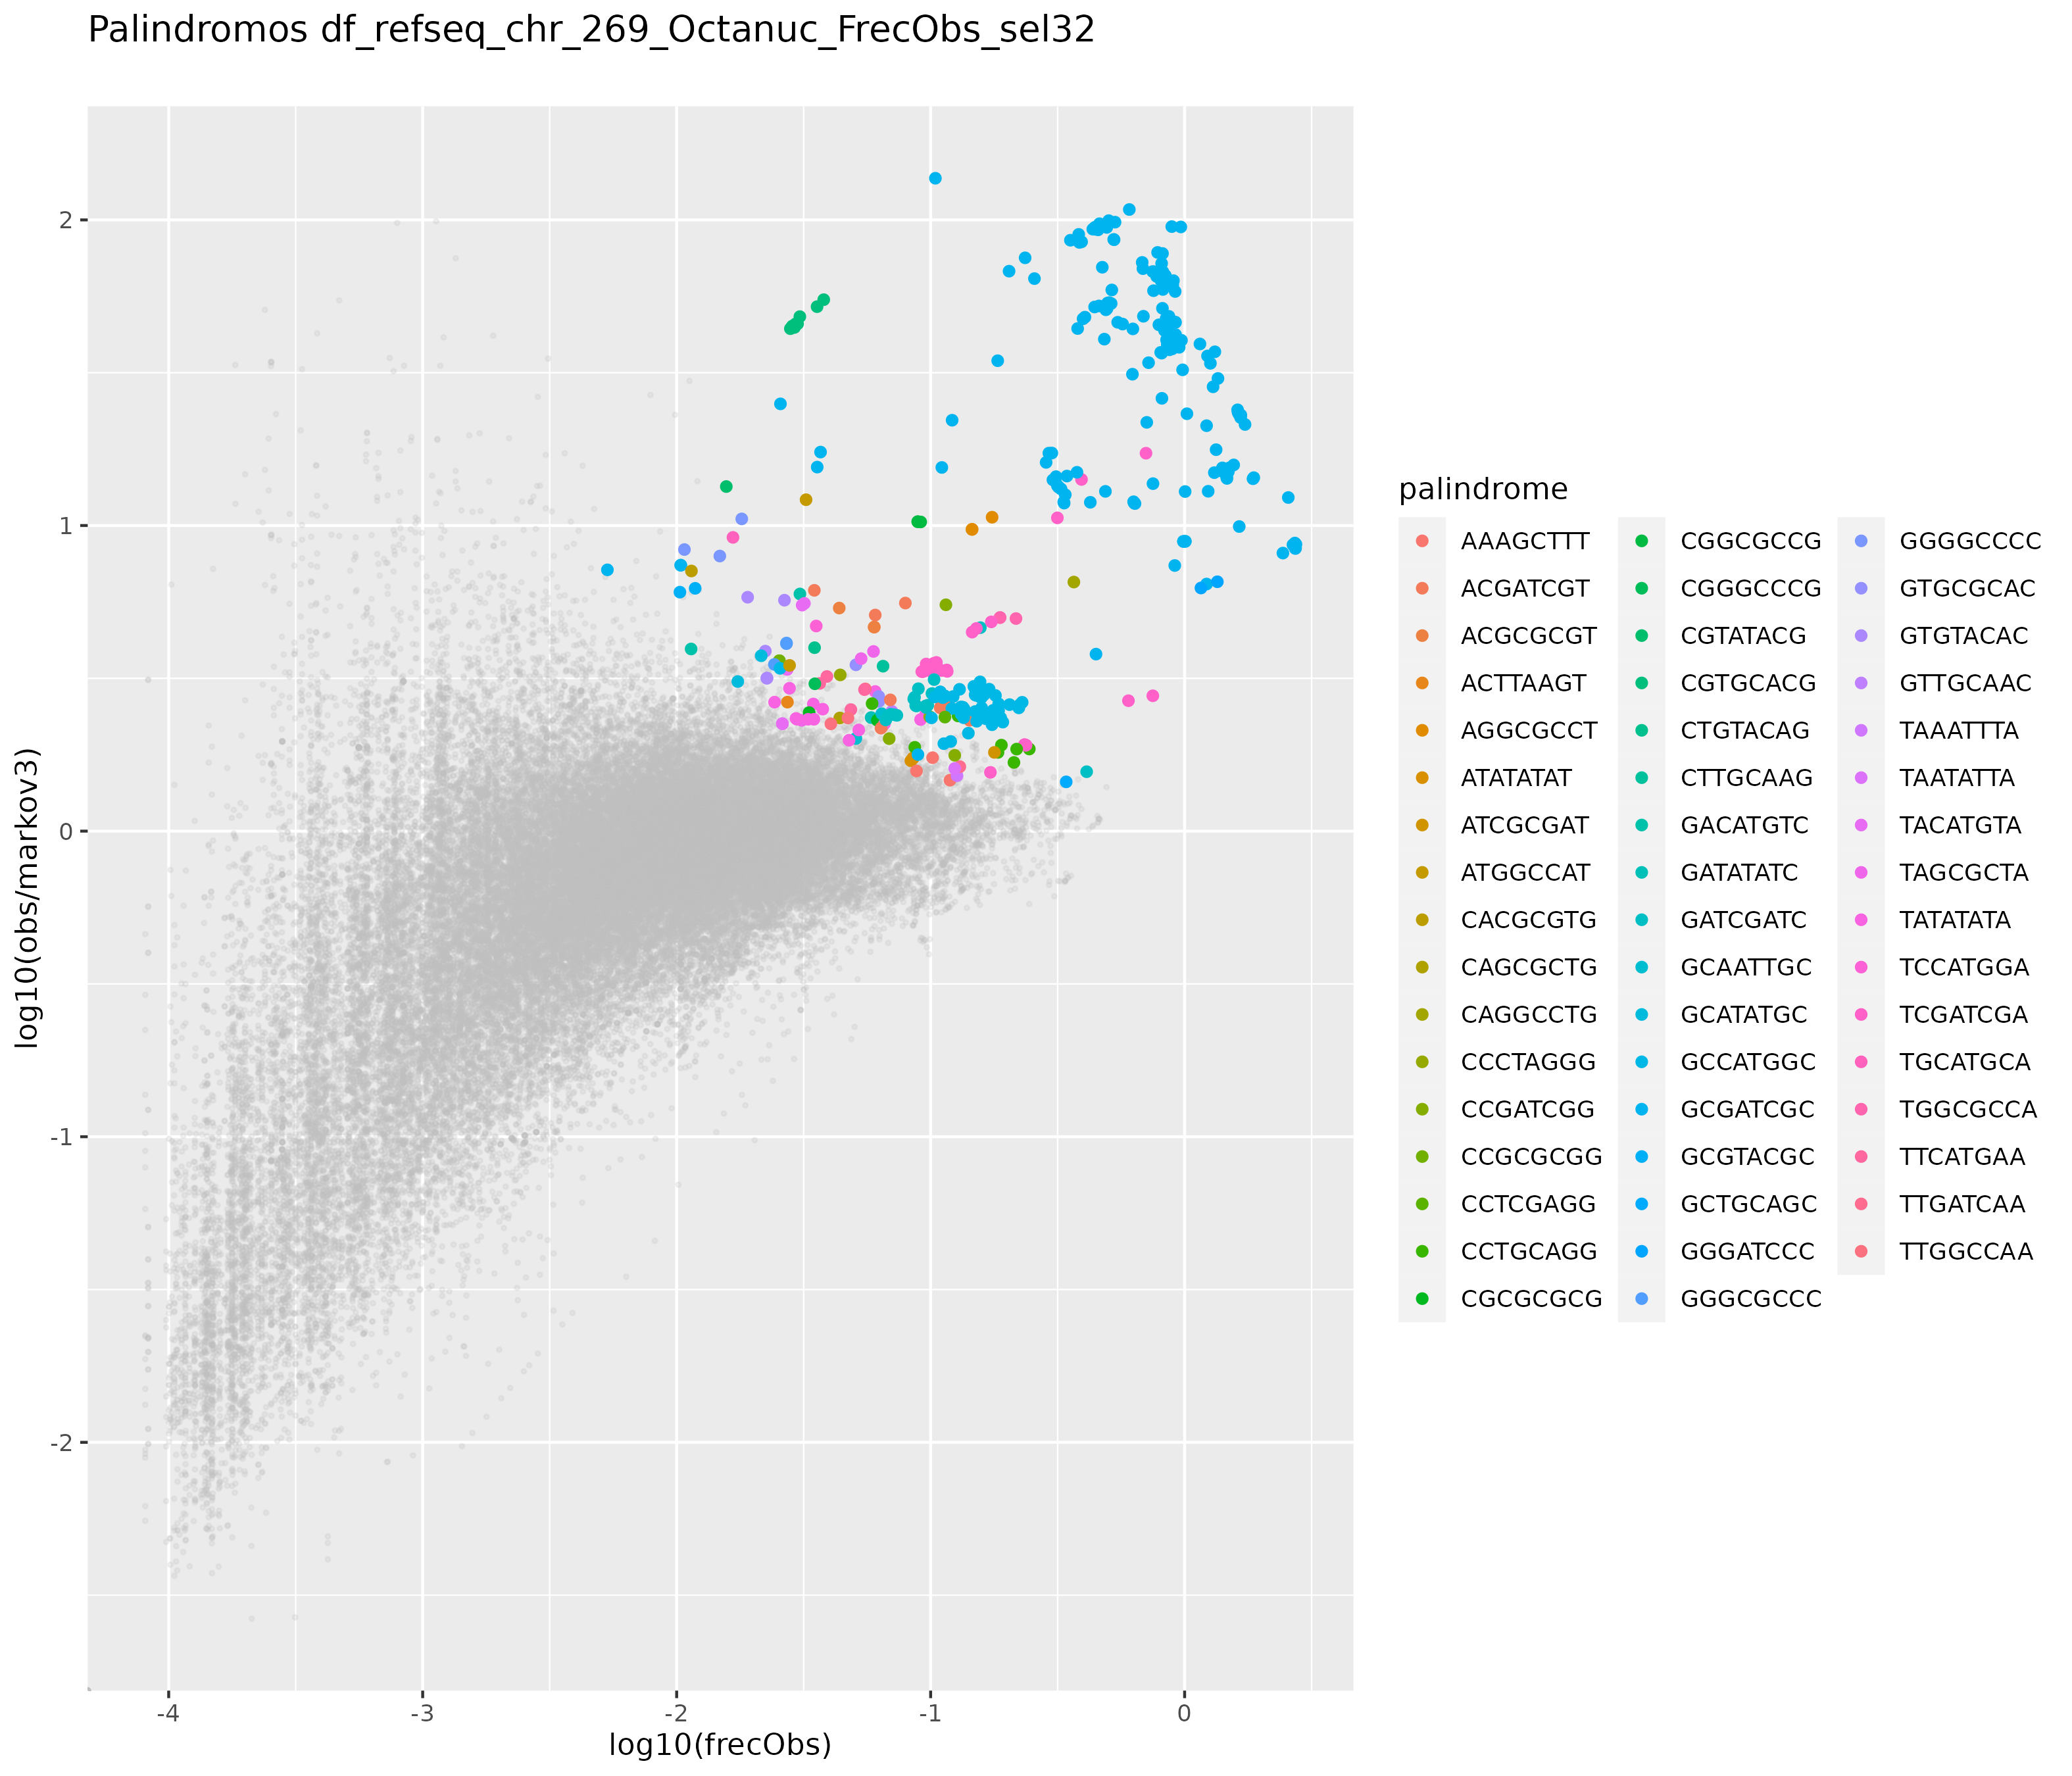
\includegraphics[width=0.8\linewidth]{figures/df_refseq_chr_269_Octanuc_FrecObs_sel32_significative-palindromes} 

}

\caption{**Enriquecimiento versus abundancia de palíndromos octámeros en el conjunto de genomas complete\_chr con un $FDR \leq 1 \times 10^{-32}$.** Enriquecimiento (**O/E**) en función de la frecuencia del motivo cada 1000 nt (**FrecObs**). Cada punto representa un palíndromo octámero de un genoma.}\label{fig:FIG1}
\end{figure}

\begin{figure}

{\centering 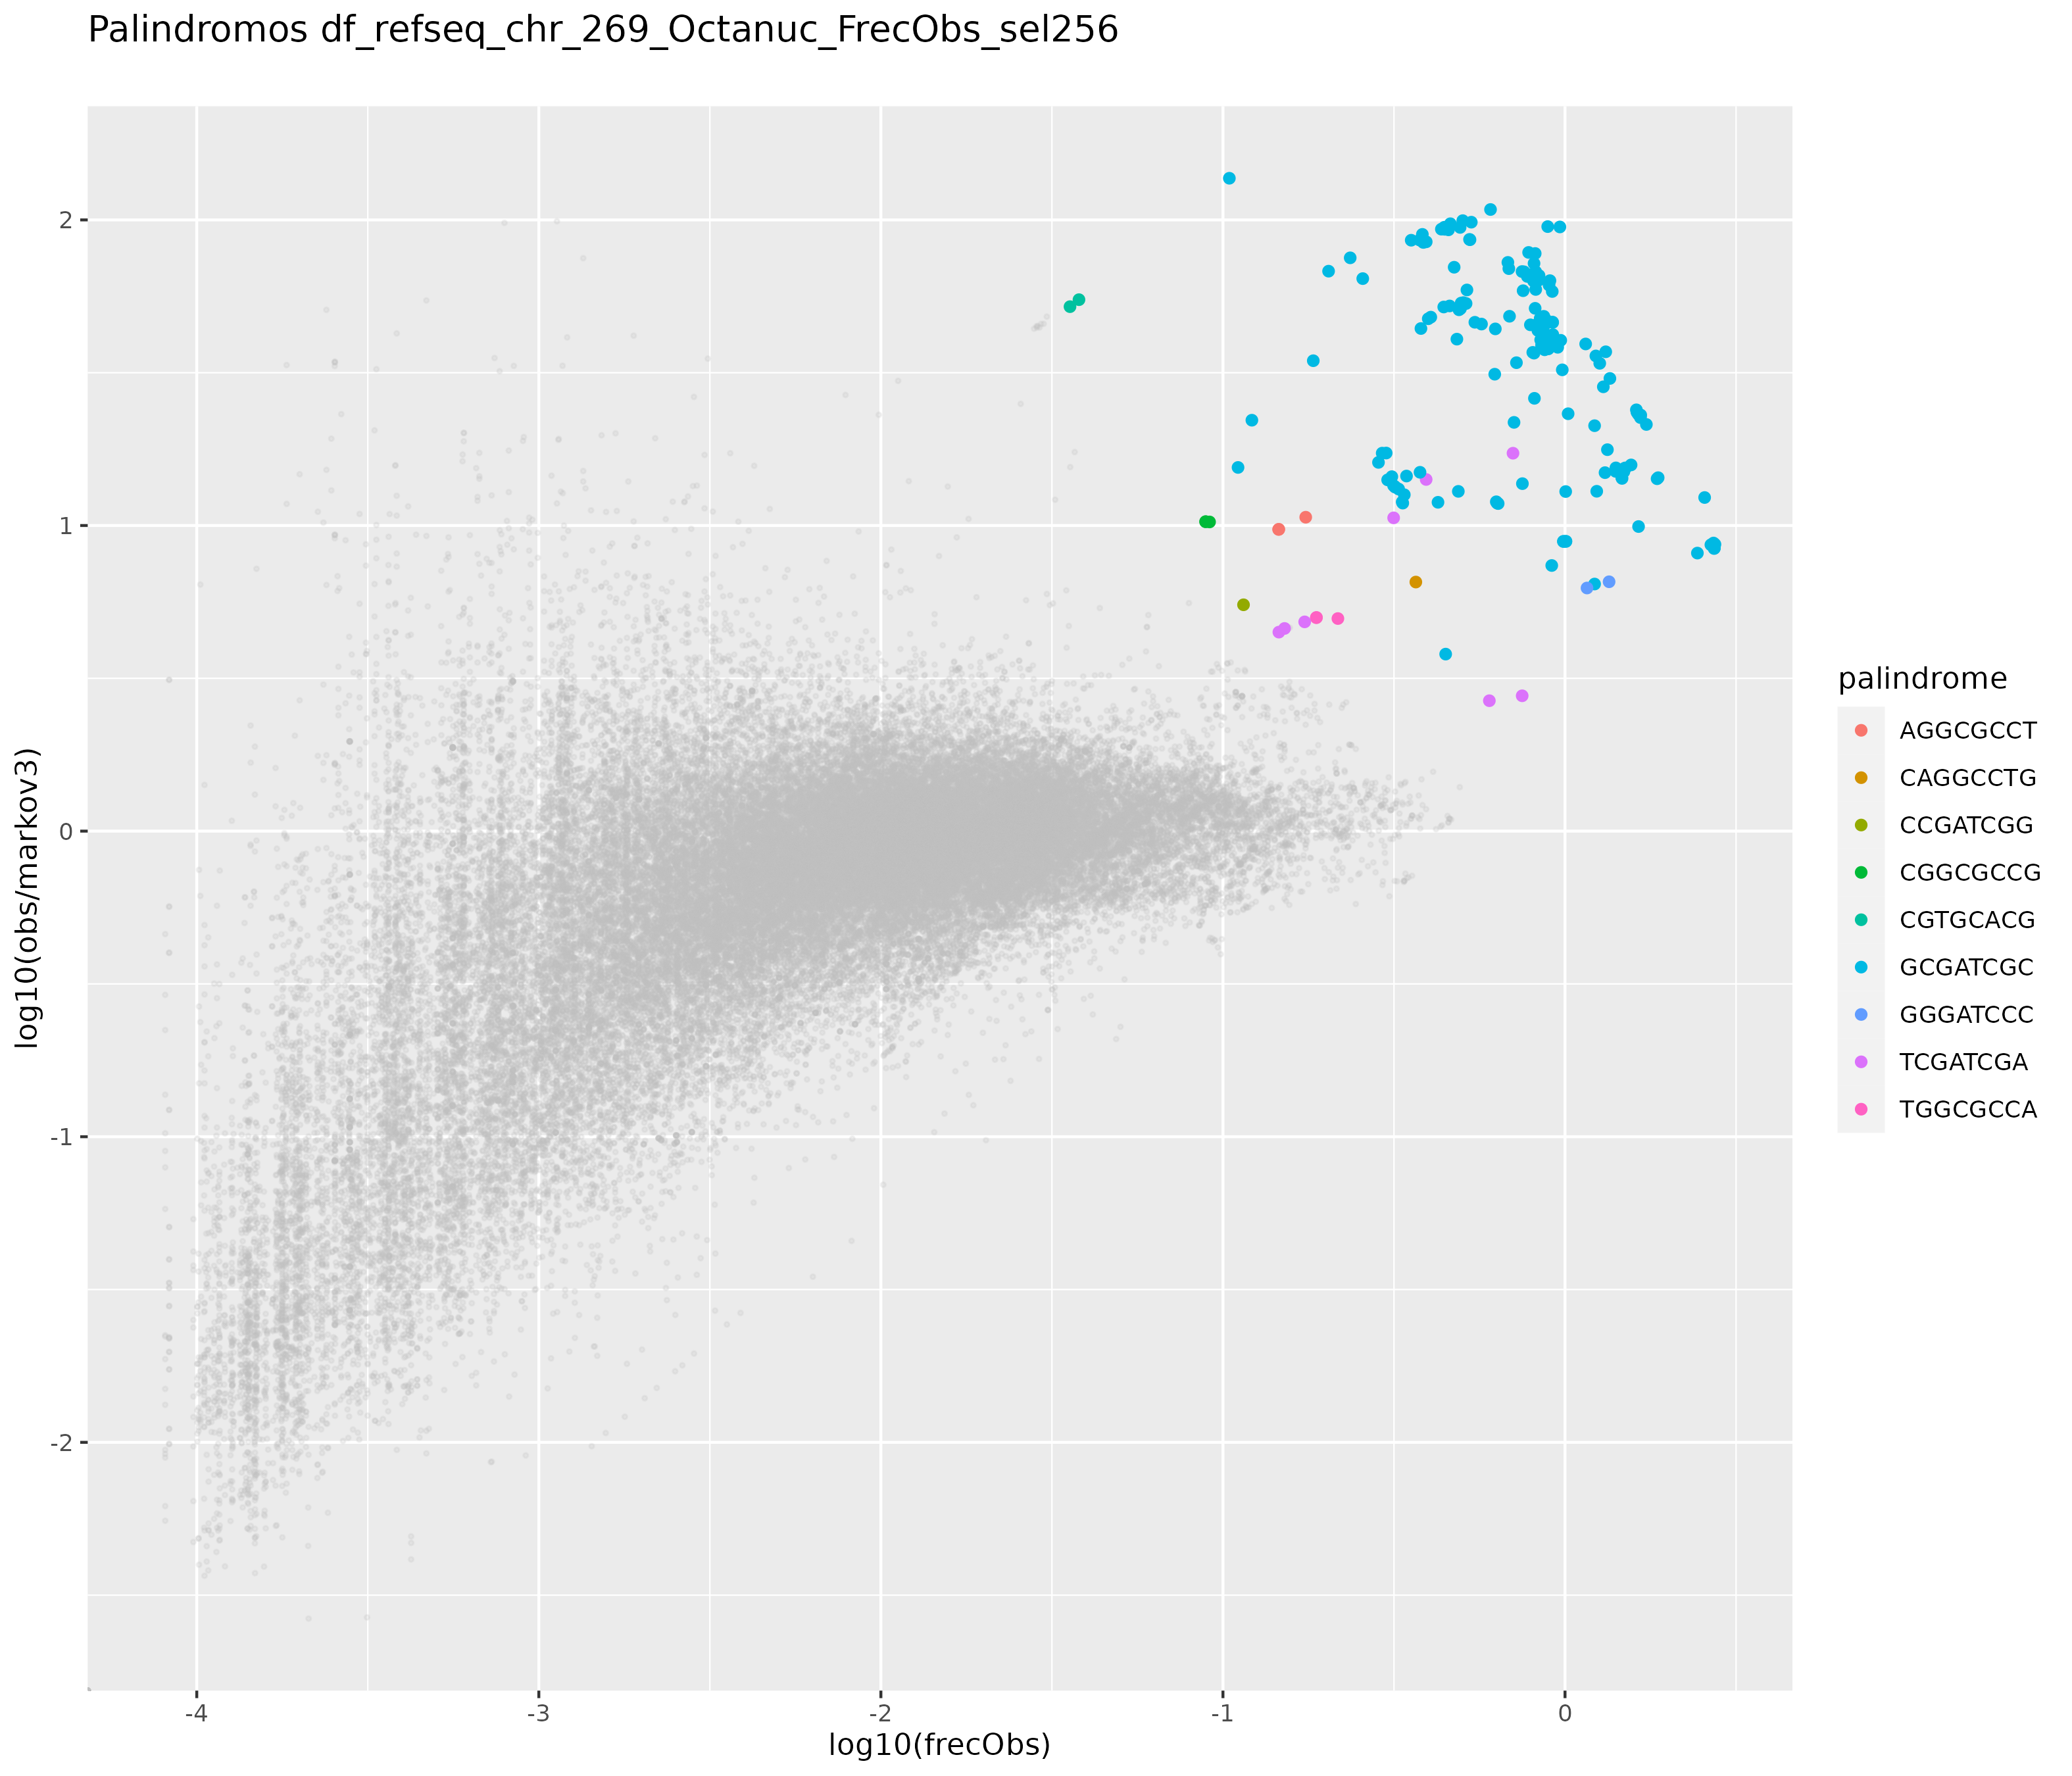
\includegraphics[width=0.8\linewidth]{figures/df_refseq_chr_269_Octanuc_FrecObs_sel256_significative-palindromes} 

}

\caption{**Enriquecimiento versus abundancia de palíndromos octámeros en el conjunto de genomas complete\_chr con un $FDR \leq 1 \times 10^{-256}$.** Enriquecimiento (**O/E**) en función de la frecuencia del motivo cada 1000 nt (**FrecObs**). Cada punto representa un palíndromo octámero de un genoma.}\label{fig:FIG2}
\end{figure}

\hypertarget{filogenia}{%
\section{Filogenia}\label{filogenia}}

Se infirieron filogenias para los dos conjuntos de genomas. Para esto usamos el software \textbf{Orthofinder} (\citet{emms2019orthofinder}), el cual utiliza \textbf{FastME} para inferir la filogenia (\citet{lefort2015fastme}). \textbf{FastME} proporciona algoritmos de distancia para inferir filogenias. FastME se basa en una evolución mínima equilibrada, que es el principio mismo de Neighbor Joining (NJ).

El software se corrió en la línea de comandos de la siguiente manera:

\begin{Shaded}
\begin{Highlighting}[]
\ExtensionTok{orthofinder}\NormalTok{ –f genomas/ }
\end{Highlighting}
\end{Shaded}

\hypertarget{anotaciuxf3n-de-la-filogenia}{%
\subsection{Anotación de la filogenia}\label{anotaciuxf3n-de-la-filogenia}}

Para tener una forma de más visual de entender la distribución de los palíndromos en los genomas, anotamos las filogenias de acuerdo a su abundancia. Se anotaron 4 filogenias según la significancia (\textbf{sel32}, \textbf{sel64}, \textbf{sel128} y \textbf{sel256}) para los 2 conjuntos de genomas. Además, esta anotación se hizo para la abundancia de acuerdo a la Frecuencia Observada por cada 1000 nucleotidos (\(FrecObs\)) (Figura \ref{fig:FIG3}) y a la tasa de Observados sobre esperados (\(OE\)) (Figura \ref{fig:FIG4}).

La anotación de las filogenias consistió en agregarles un heatmap que mostrara la abundancia de cada palíndromo y un diagrama de barras que indicara aquel palíndromo con mayor abundancia.

\begin{figure}

{\centering 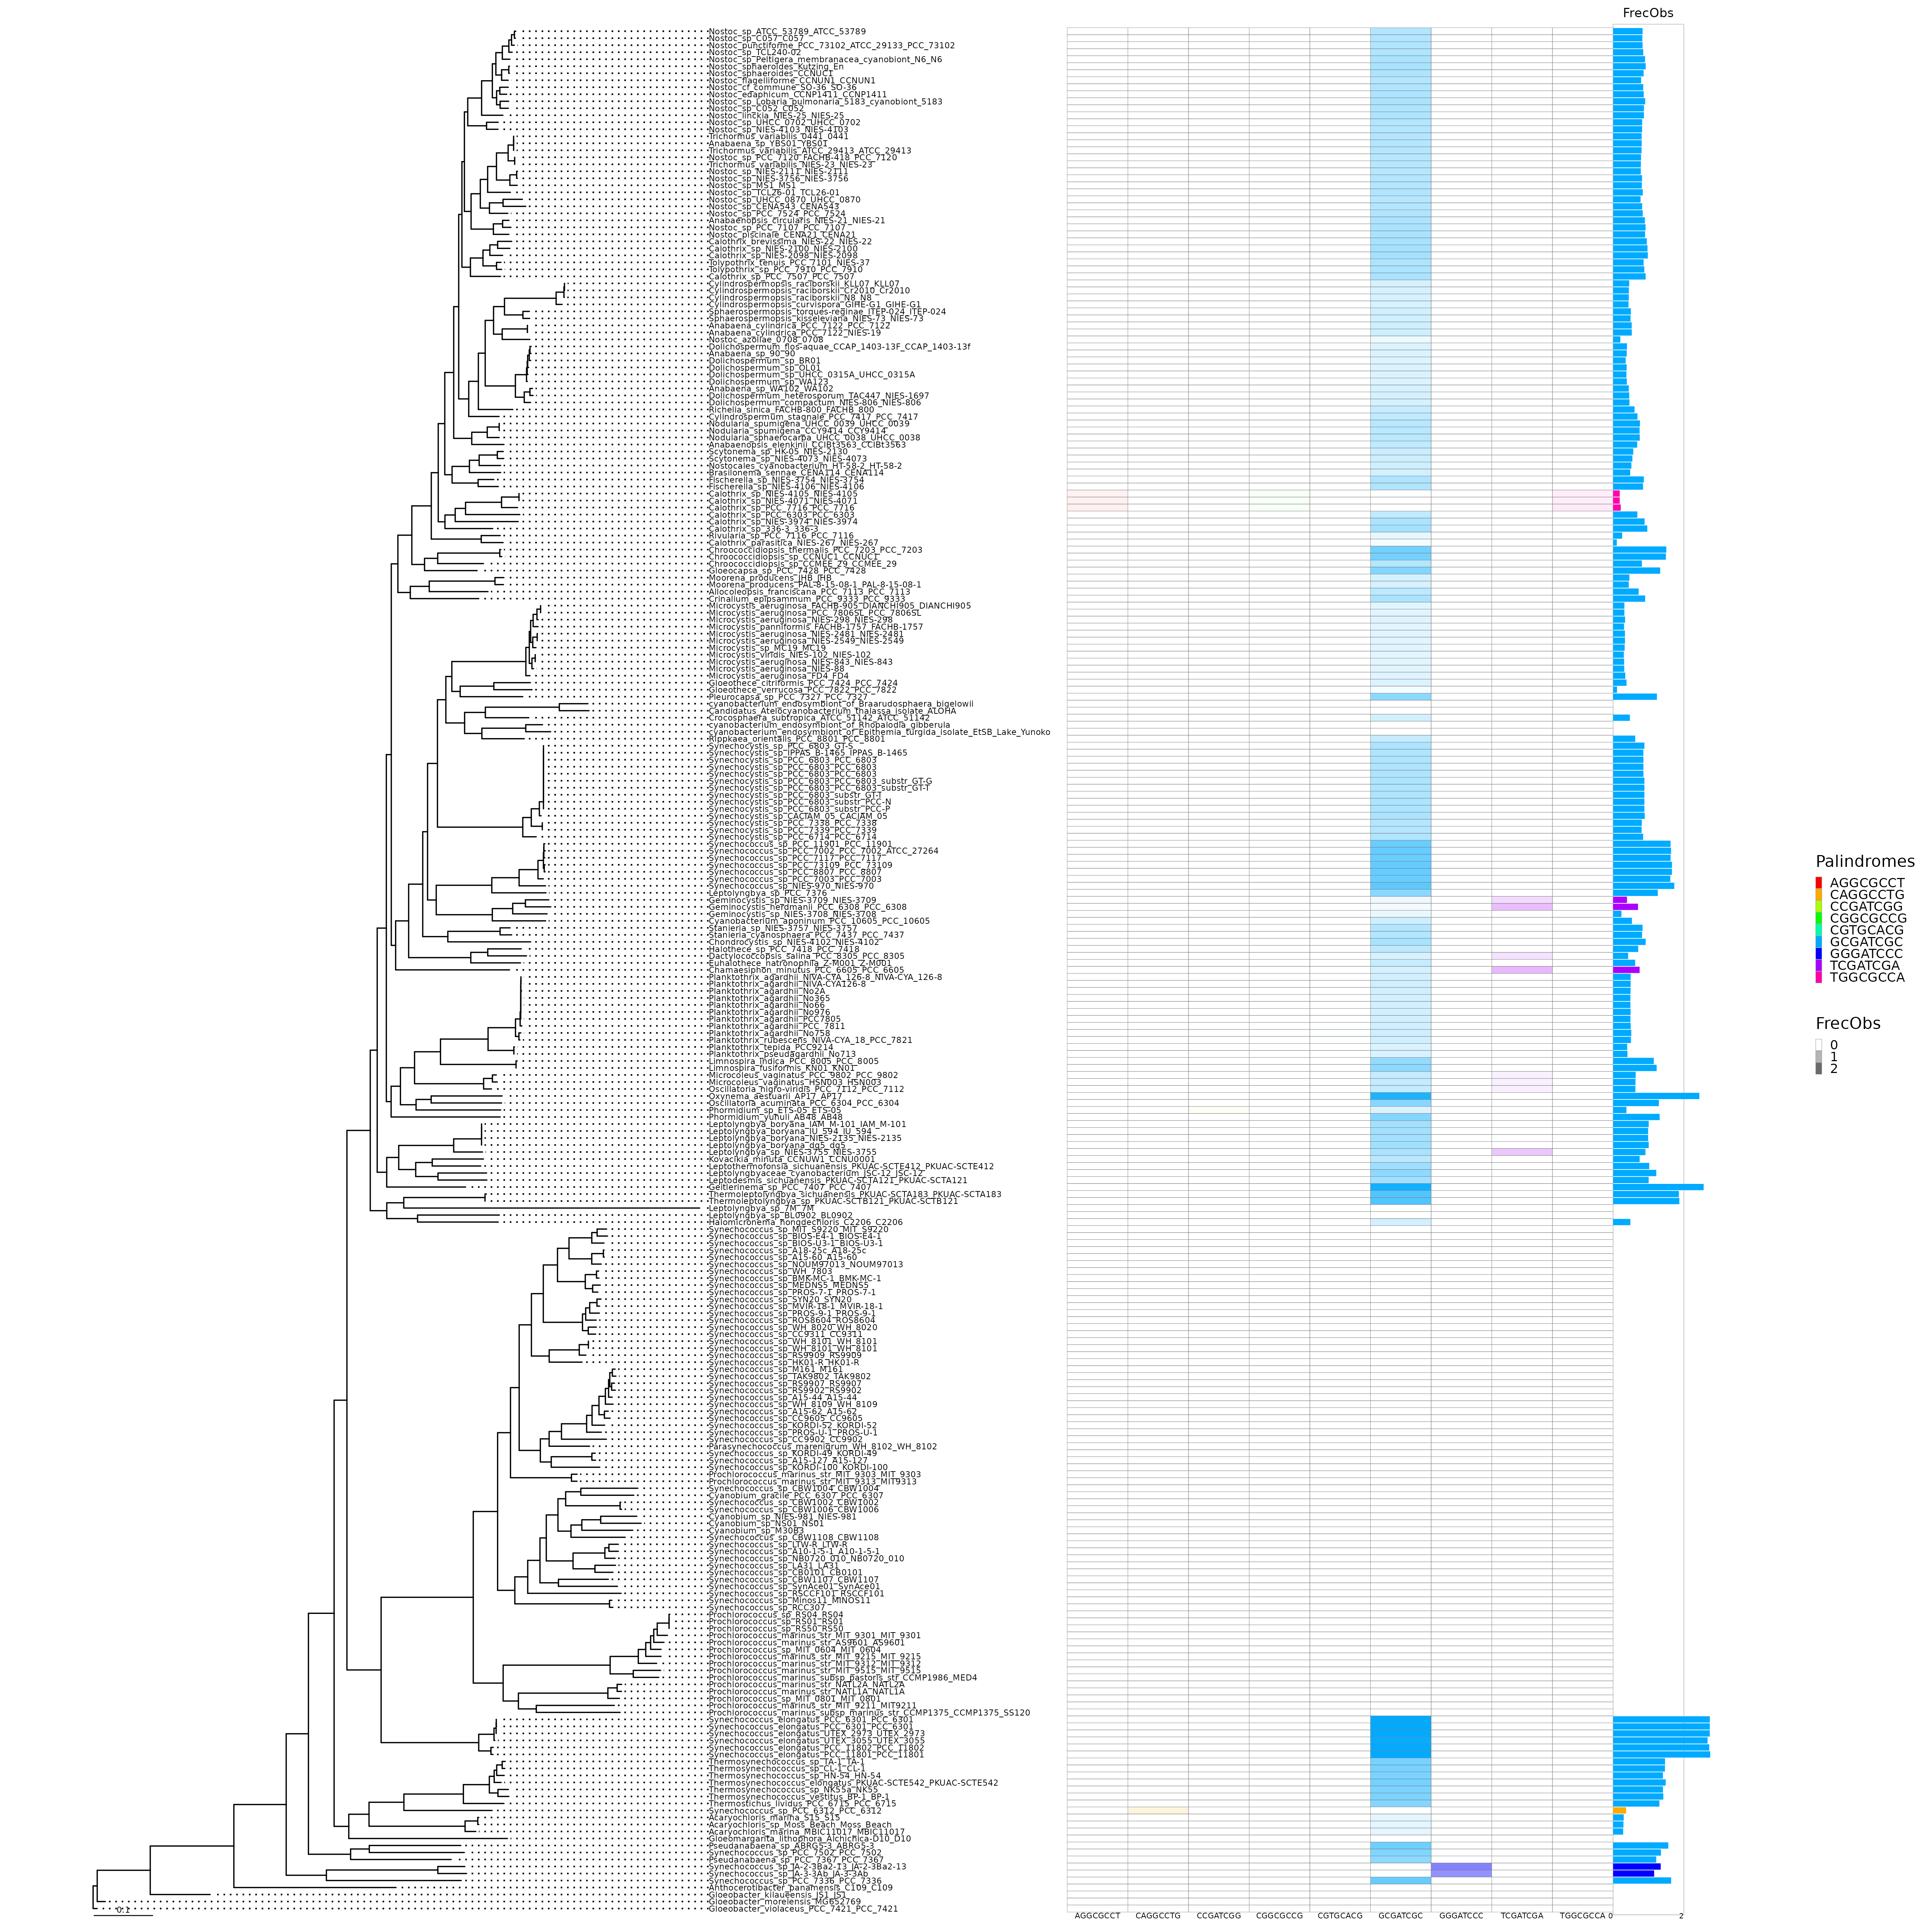
\includegraphics[width=75in]{figures/refseq_chr_269_Octanuc_FrecObs_sel256_filogenia_HIG} 

}

\caption{**Filogenia del conjunto de genomas *complete\_chr* anotada de acuerdo a la Frecuencia observada cada 1000 nt (FrecObs).** La abundancia visualizada en esta filogenia es de acuerdo al conjunto **sel256**, es decir conteos con un $FDR \leq 1 \times 10^{-256}$. La filogenia muestra 269 especies, frente a la filogenia se muestra un heatmap que indica la abundancia de cada palíndromo. Frente al Heatmap se muestra un Diagrama de barras el cual indíca el palindromo mas abundante de entre todos.}\label{fig:FIG3}
\end{figure}

\begin{figure}

{\centering 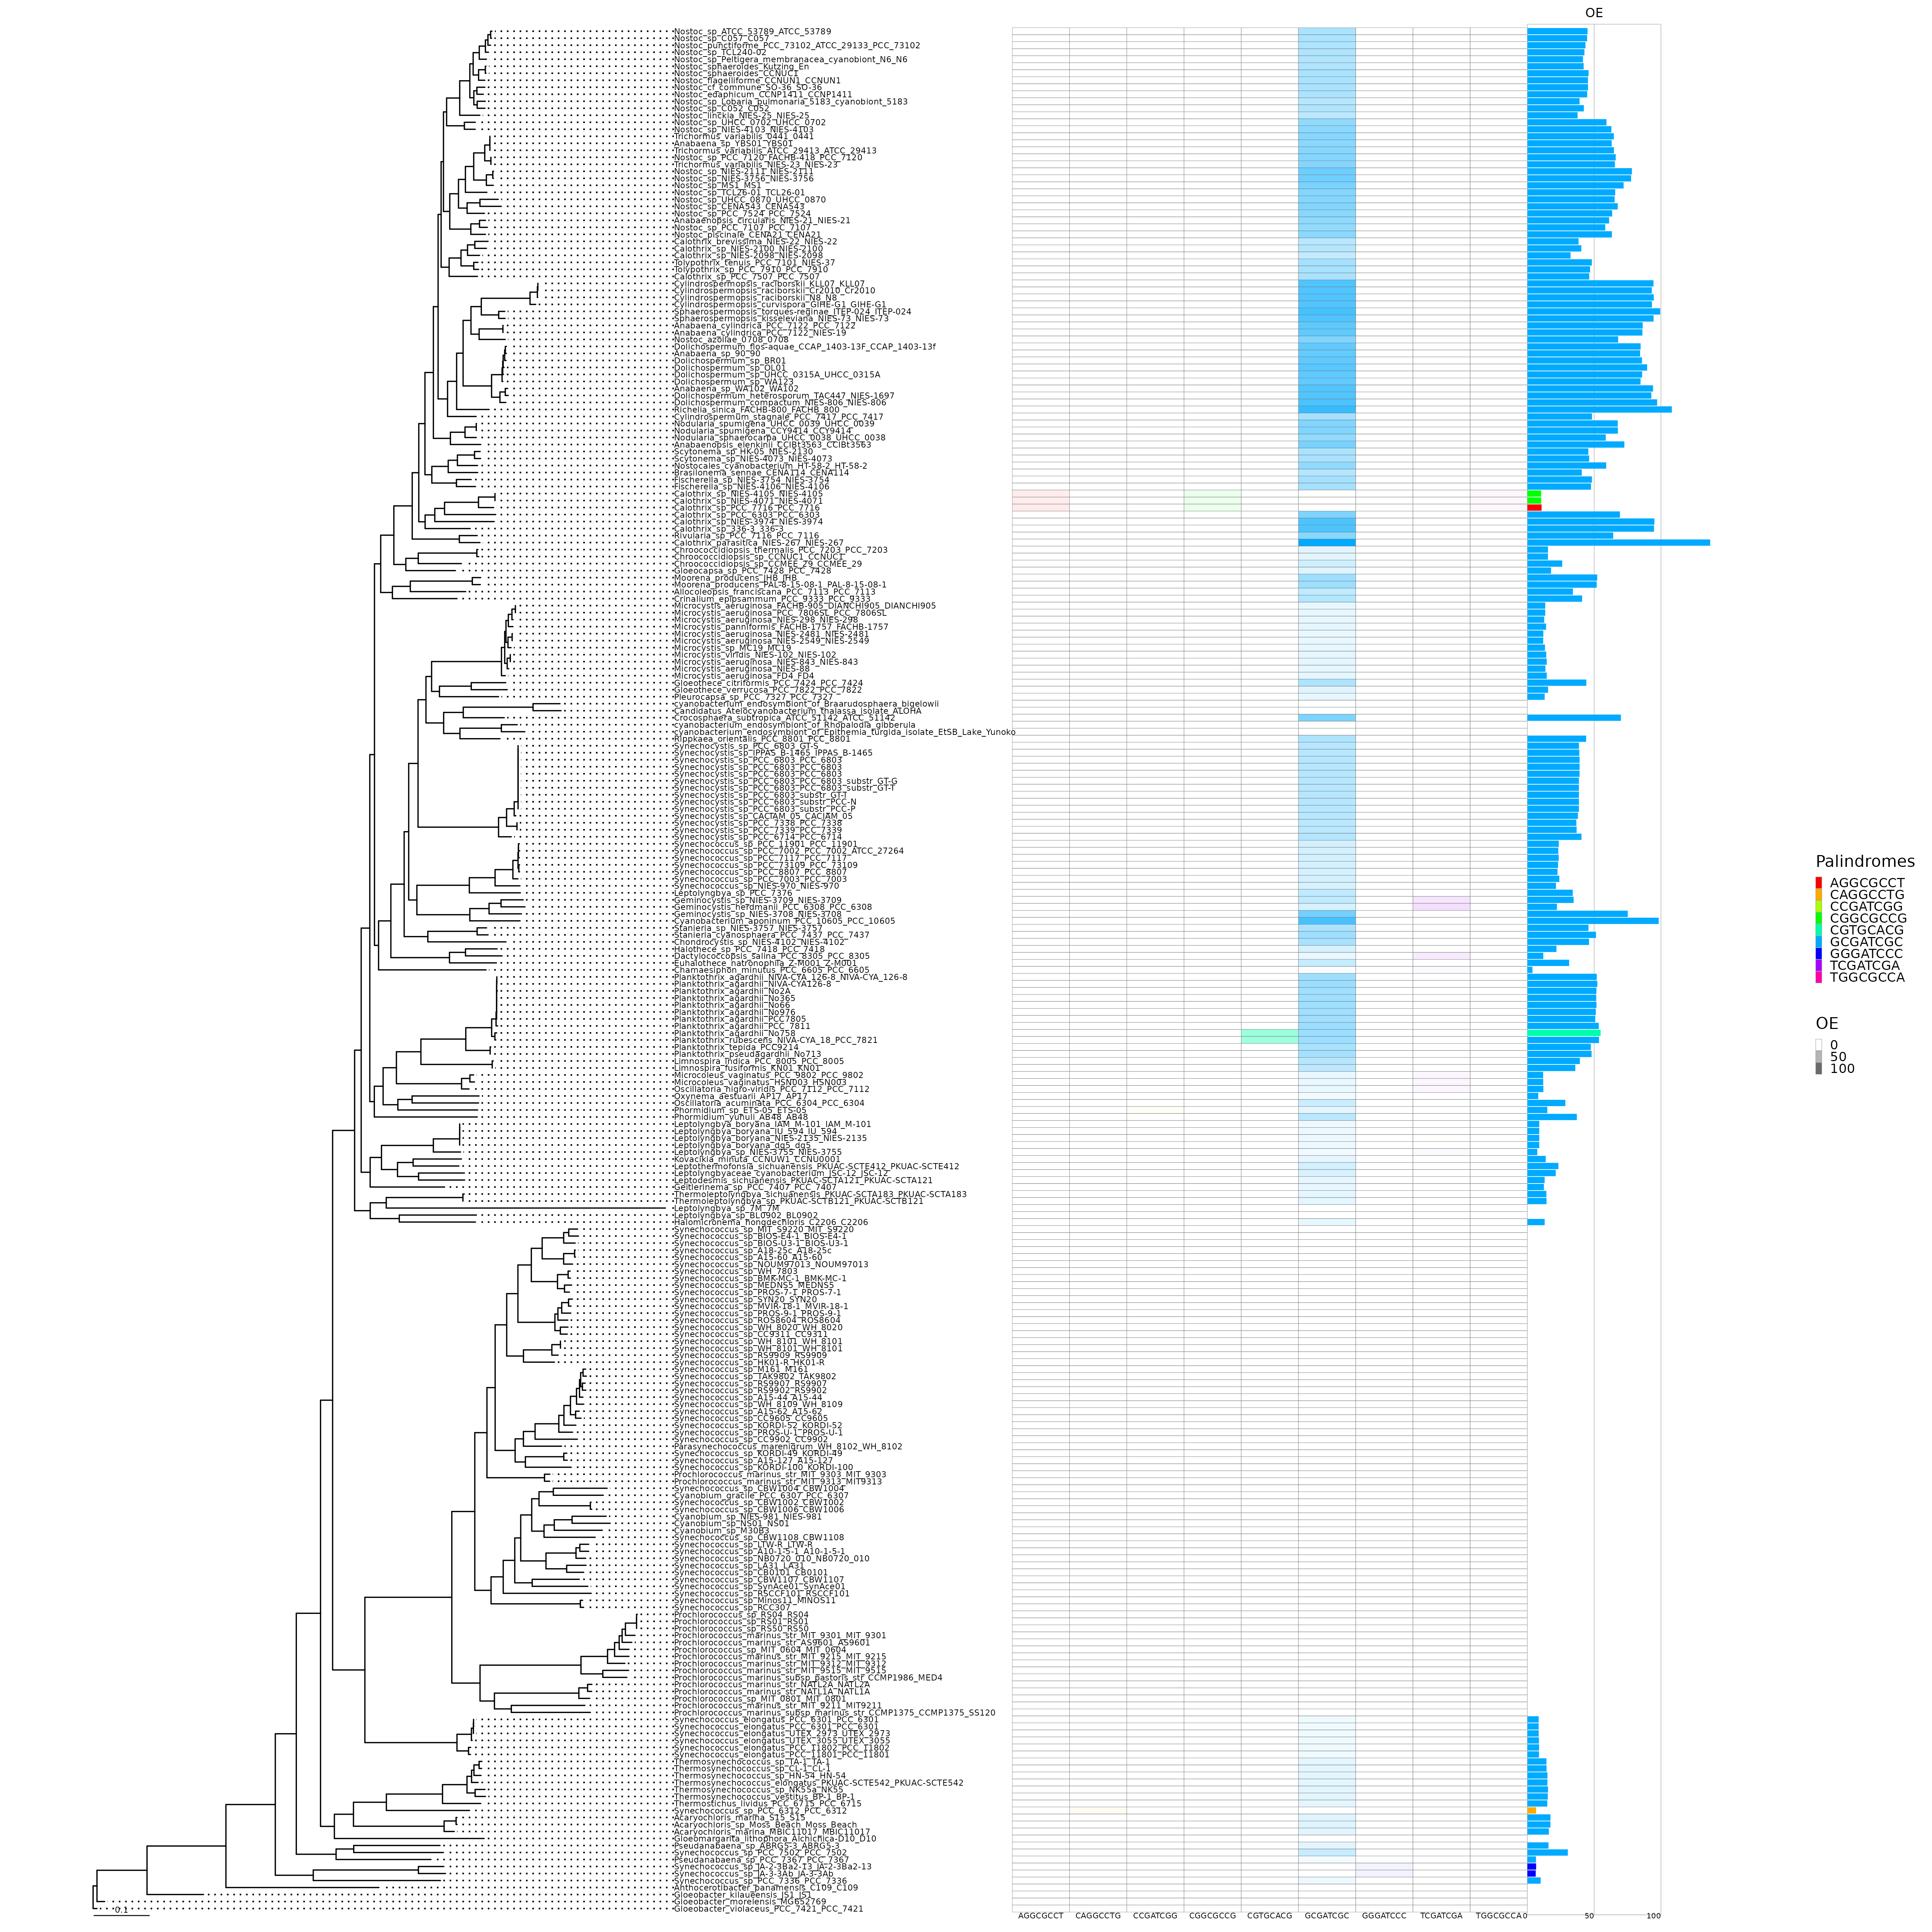
\includegraphics[width=75in]{figures/refseq_chr_269_Octanuc_OE_sel256_filogenia_HIG} 

}

\caption{**Filogenia del conjunto de genomas *complete\_chr* anotada de acuerdo a la tasa de observados sobre esperados (OE).** La abundancia visualizada en esta filogenia es de acuerdo al conjunto **sel256**, es decir conteos con un $FDR \leq 1 \times 10^{-256}$. La filogenia muestra 269 especies, frente a la filogenia se muestra un heatmap que indica la abundancia de cada palíndromo. Frente al Heatmap se muestra un Diagrama de barras el cual indíca el palindromo mas abundante de entre todos.}\label{fig:FIG4}
\end{figure}

\hypertarget{identificaciuxf3n-de-casos-relevantes}{%
\section{Identificación de casos relevantes}\label{identificaciuxf3n-de-casos-relevantes}}

De acuerdo a las filogenias anotadas, se buscaron aquellos casos en los que HIP1 o algún otro palíndromo se hubiera ganado o perdido abruptamente y en su lugar hubiese otro palíndromo abundante. Además, se buscó que en aquellos casos, las ramas en la filogenia no fueran tan largas. Esto se hizo de manera visual revisando el diagrama de barras que mostraba el palíndromo más abundante para cada especie. En total hubo 6 subclados que mostraban cambios abruptos en la abundancia de sus palíndromos (Figura \ref{fig:FIG5}).

\begin{figure}

{\centering 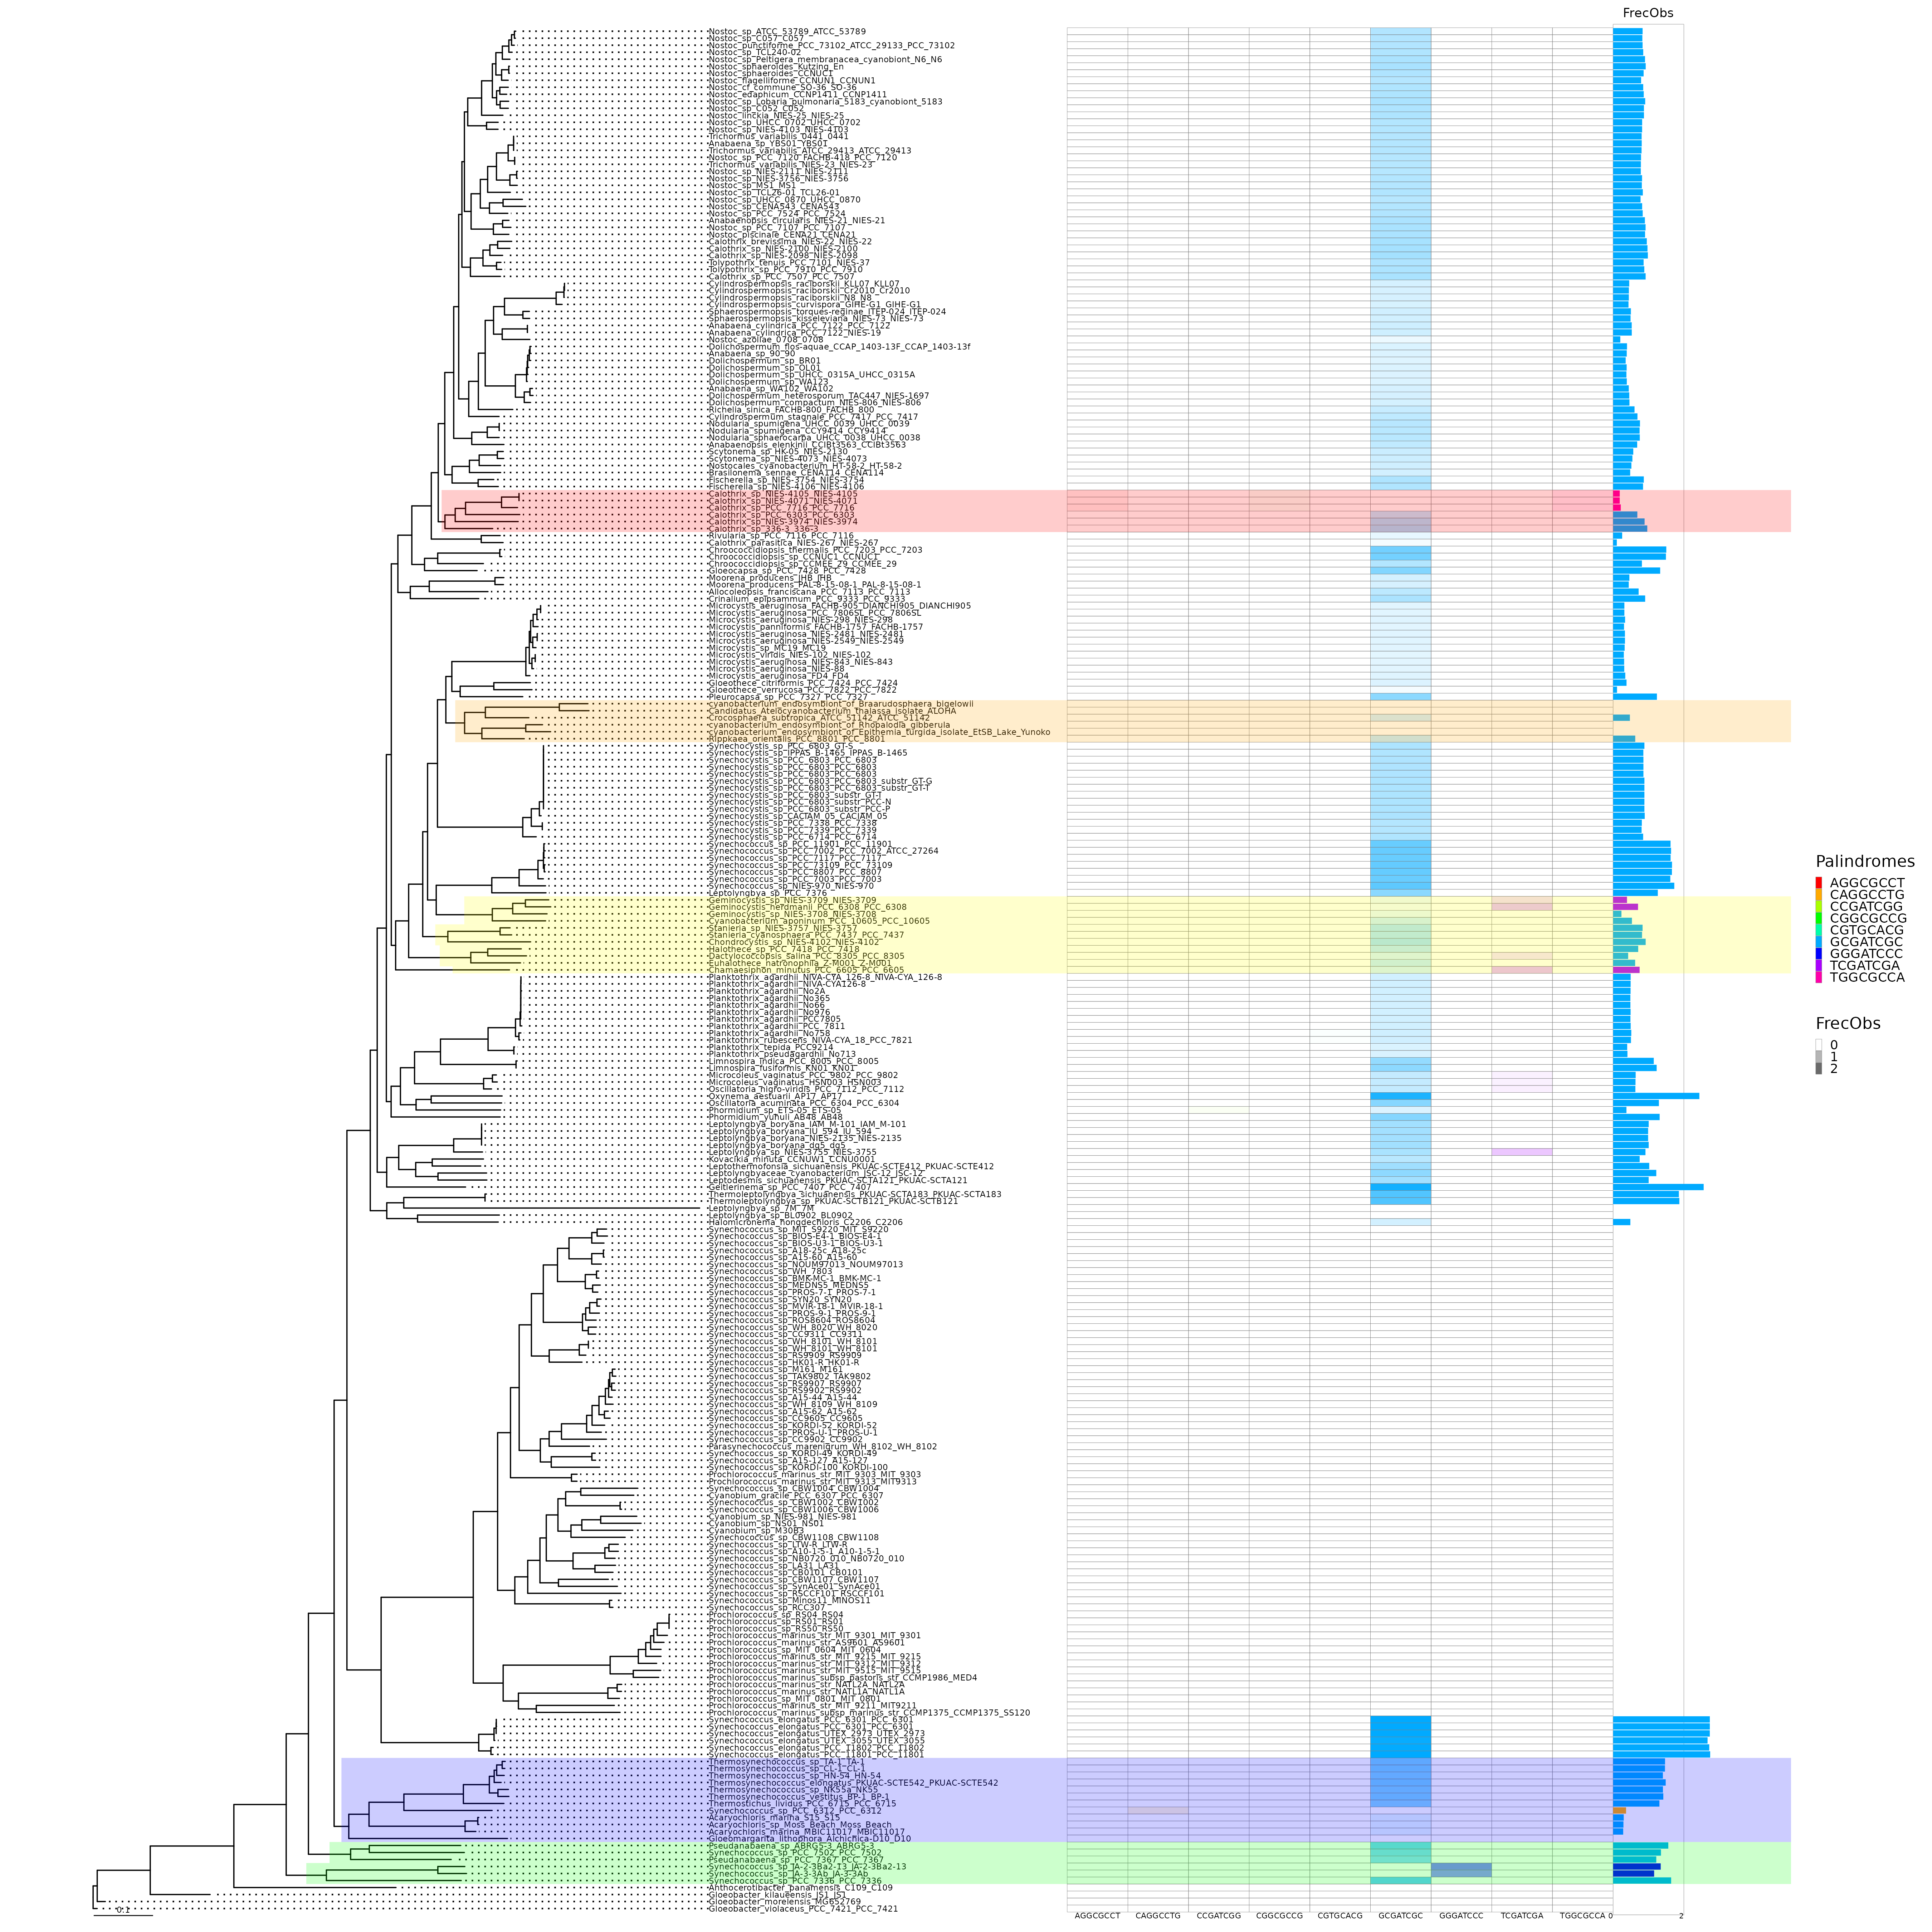
\includegraphics[width=75in]{figures/refseq_chr_269_Octanuc_FrecObs_sel256_filogenia_HIG_cases} 

}

\caption{**Casos de interés.** En la figura se muestran remarcados los casos interesantes: **clado calothrix** (rojo), **clado cyanobacterium** (naranja), **clado geminocystis** (amarillo), **clado thermosynechococcus** (azul), **clado pseudoanabaena** (verde).}\label{fig:FIG5}
\end{figure}

También se hallo un caso interesante en el conjunto \textbf{pico} (\textbf{clado A18-40}) el cual sirvió como punto de partida para analisis posteriores. En este caso se muestra que la especie Synechococcus A18-40 muestra una tasa OE mucho mayor comparada con las demás especies del clado (Figura \ref{fig:FIG6}).

\begin{figure}

{\centering 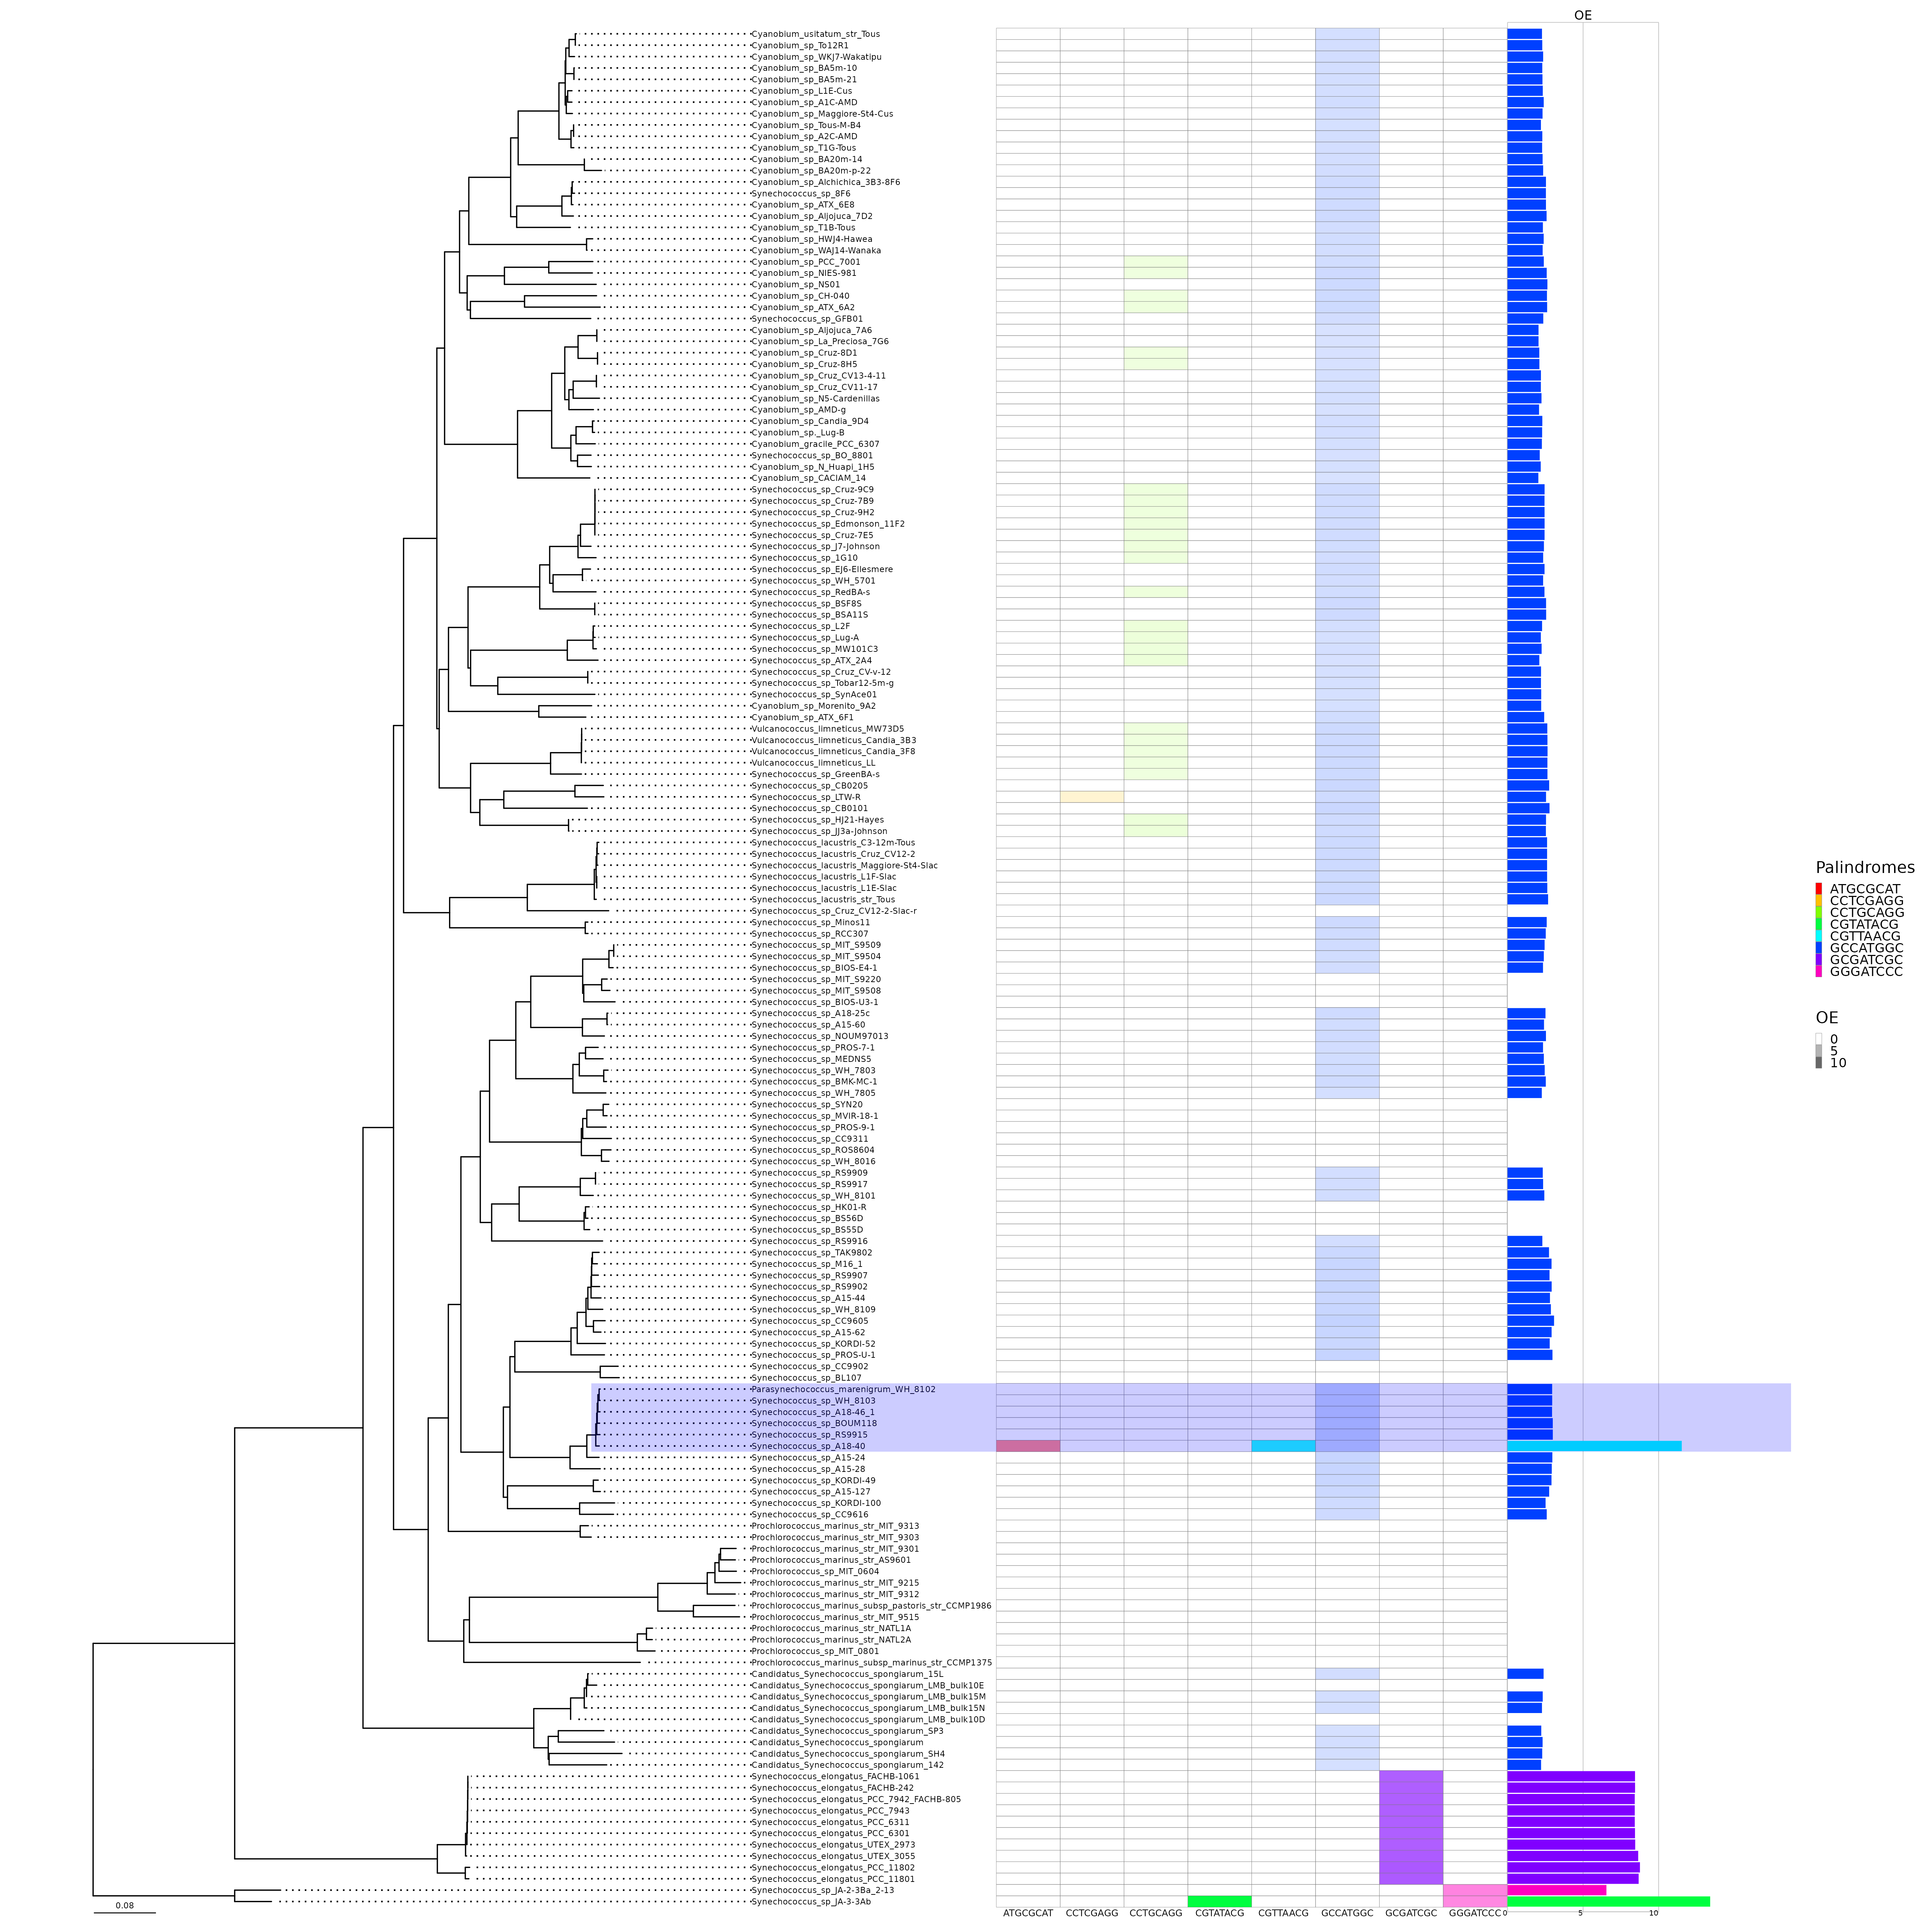
\includegraphics[width=75in]{figures/pico_165_Octanuc_OE_sel32_filogenia_HIG_cases} 

}

\caption{**Casos de interés.** En la figura se muestra remarcado el **clado A18-40** (azul).}\label{fig:FIG6}
\end{figure}

\hypertarget{reconstrucciuxf3n-ancestral-de-sitios-palindruxf3micos-en-ortuxf3logos}{%
\section{Reconstrucción Ancestral de sitios palindrómicos en ortólogos}\label{reconstrucciuxf3n-ancestral-de-sitios-palindruxf3micos-en-ortuxf3logos}}

Para tratar de entender como es que los sitios HIP1 han ido evolucionando, hicimos una reconstrucción de sitios ancestrales y posteriormente construimos varios conjuntos de redes para visualizar dicha evolución.

\hypertarget{ortuxf3logos}{%
\subsection{Ortólogos}\label{ortuxf3logos}}

Para simplificar la reconstrucción de secuencias ancestrales usamos unicamente los ortólogos. Para obtener esto usamos el pipeline \texttt{get\_homologues}:

\begin{Shaded}
\begin{Highlighting}[]
\ExtensionTok{get\_homologues.pl} \AttributeTok{{-}d}\NormalTok{ gbff }\AttributeTok{{-}t}\NormalTok{ 0 }\AttributeTok{{-}M} \AttributeTok{{-}n}\NormalTok{ PPN}
\end{Highlighting}
\end{Shaded}

Después de obtener los ortólgos filtramos:

\begin{itemize}
\tightlist
\item
  aquellos que no estuvieran en las 6 especies del clado
\item
  aquellos que tuvieran mas de una copia (parálogos)
\item
  aquellos sin sitios HIP1
\end{itemize}

\hypertarget{reconstrucciuxf3n}{%
\subsection{Reconstrucción}\label{reconstrucciuxf3n}}

Para hacer la reconstrucción usamos la pagueteria de R \texttt{phangorn}, la cual proporciona varios métodos para estimar estados de caracteres ancestrales con Máxima Parsimonia (MP) o Máxima Verosimilitud (ML). En este caso usamos ML. Adicionalmente podemos asignar los estados ancestrales según la máxima verosimilitud (``ml''):
\[P(x_r=A) = {{L(x_r=A)} \over {\sum\limits_{k\in \{A,C,G,T\}}} L(x_r= k) }\]

y el criterio de mayor probabilidad posterior (``bayes''):
\[P(x_r=A) = {{\pi_A L(x_r=A)} \over {\sum\limits_{k\in \{A,C,G,T\}}} \pi_k L(x_r= k) }\]

dónde \(L(x_r)\) es la probabilidad conjunta de los estados en las puntas y el estado en la raíz \(x_r\) y \(\pi_i\) son las frecuencias base estimadas del estado \(i\).

Toda la información de la reconstrucción fue guardada en dos tablas las cuales contienen listas de cada transicion entre cada estado. Estas tablas fueron creadas con la siguiente función:

\begin{Shaded}
\begin{Highlighting}[]
\FunctionTok{source}\NormalTok{(}\StringTok{"ASR\_Orth\_Functions/NodeAndEdges.R"}\NormalTok{)}

\FunctionTok{Create\_Transition\_Table}\NormalTok{ (}\AttributeTok{SitesTable =} \StringTok{"Clados/Callothrix\_clade/PALINDROMES/GCGATCGC/Orthologues\_Palindrome\_sites.txt"}\NormalTok{,}
                                \AttributeTok{EvolutionModel =} \StringTok{"F81"}\NormalTok{,}
                                \AttributeTok{Method =} \StringTok{"bayes"}\NormalTok{,}
                                \AttributeTok{Phylogeny =} \StringTok{"Clados/Callothrix\_clade/SpeciesTree\_rooted.txt"}\NormalTok{,}
                                \AttributeTok{OrthoPath =} \StringTok{"Clados/Callothrix\_clade/PALINDROMES/GCGATCGC/Only\_ORTHOLOGUES/"}\NormalTok{)}
\end{Highlighting}
\end{Shaded}

\hypertarget{resultados}{%
\chapter{RESULTADOS}\label{resultados}}

Acontinucación se presentan los resultados en cuatro secciones:

\begin{itemize}
\item
  La \textbf{Seccion I} muestra los analisis de la distribución de los sitios palindromicos a través de los ortólogos y marcos de lectura de las especies.
\item
  La \textbf{Sección II} muestra una serie de resultados de la reconstrucción ancestral de los sitios palindrómicos HIP1 y TGGCGCCA unicamente para el clado Calothrix.
\item
  La \textbf{Sección III} muestra una serie de resultados de la reconstrucción ancestral de los sitios palindrómicos HIP1 y TGGCGCCA unicamente para el clado Thermosynechococcus.
\item
  La \textbf{Sección IV} muestra los resultados del análisis de sitios CGTTAACG en el clado A18-40.
\item
  La \textbf{Sección V} muestra los resultados del análisis de sitios repetidos en el los clados.
\item
  La \textbf{Sección VI} muestra una serie de resultados de la reconstrucción ancestral de los sitios palindrómicos HIP1 para los clados Cyanobacterium, Geminocystis y Pseudoanabaena.
\end{itemize}

\hypertarget{secciuxf3n-i}{%
\chapter*{Sección I}\label{secciuxf3n-i}}
\addcontentsline{toc}{chapter}{Sección I}

\hypertarget{distribuciuxf3n-de-hip1-en-los-marcos-de-lectura}{%
\section{Distribución de HIP1 en los marcos de lectura}\label{distribuciuxf3n-de-hip1-en-los-marcos-de-lectura}}

Para el analisis de los sitios palindrómicos primero se hizo un conteo de lo sitios en cada especie de cada clado para luego tomar aquella especie que tuviera la mayor cantidad de sitios posibles. Esto con el fin de tener mas sitios para analizar. Aquellas especies con la mayor cantidad de sitios se muestran resaltadas en amarillo en la Tabla \ref{tab:HighestSites}.

Para ver como es la distribución de los sitios HIP1 a traves del genoma hicimos un conteo de sitios en cada marco de lectura (Tabla \ref{tab:TABMuts2}).

\hypertarget{secciuxf3n-ii}{%
\chapter*{Sección II}\label{secciuxf3n-ii}}
\addcontentsline{toc}{chapter}{Sección II}

\hypertarget{clado-calothrix}{%
\section{Clado Calothrix}\label{clado-calothrix}}

El clado calothrix contiene 6 especies y es de interes ya que segun la filogenia estan estrechamente relacionadas y muestra un cambio en el palindromo mas abundante, pasando de \textbf{GCGATCGC} a \textbf{TGGCGCCA} (Figure \ref{fig:FIG12}).

\begin{figure}

{\centering 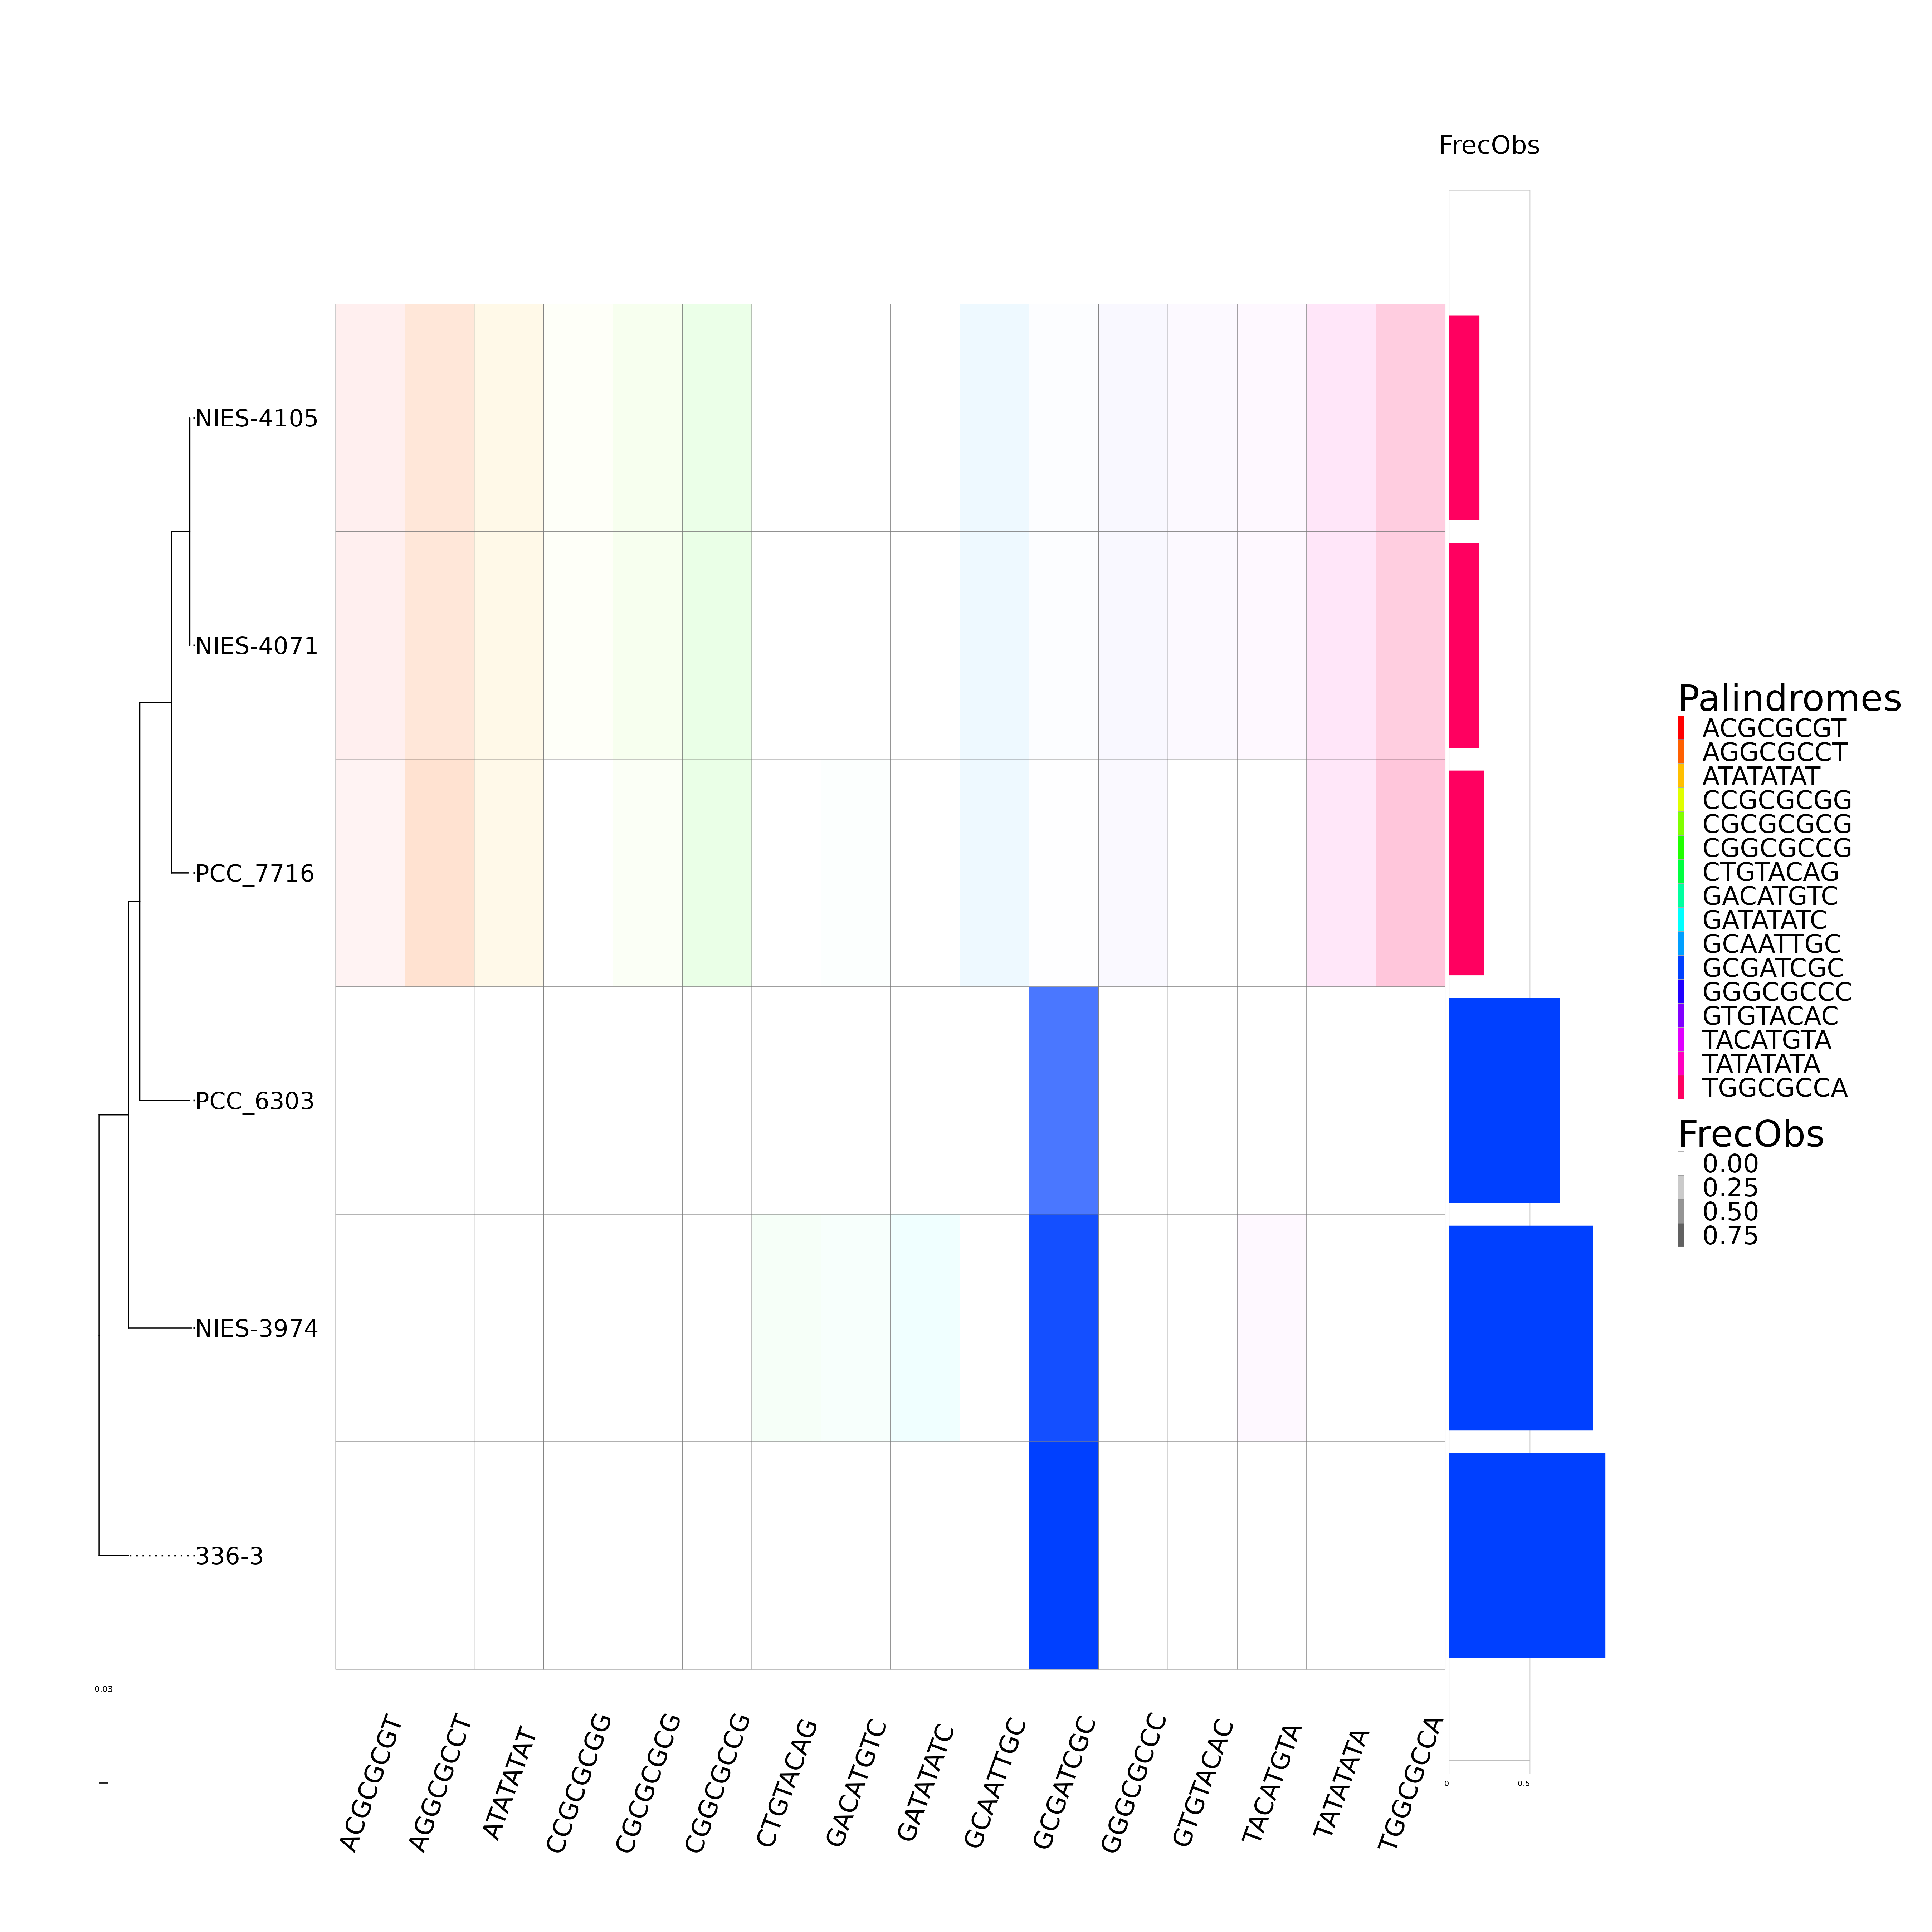
\includegraphics[width=1\linewidth]{Clados/Callothrix_clade/figures/Calothrix_Octanuc_FrecObs_sel32_filogenia_HIG} 

}

\caption{**Filogenia anotada del clado Calothrix.** En esta imagen se muestra un cambio abrupto en la Frecuencia observada de **GCGCATCGC** en las especies NIES-4105, NIES-4071 y PCC\_7716.}\label{fig:FIG12}
\end{figure}

\hypertarget{conjunto-de-sitios-hip1-usando-la-especie-336-3-como-referencia}{%
\subsection{Conjunto de sitios HIP1 usando la especie 336-3 como referencia}\label{conjunto-de-sitios-hip1-usando-la-especie-336-3-como-referencia}}

\hypertarget{red-de-transiciones}{%
\subsubsection{Red de transiciones}\label{red-de-transiciones}}

Para hacer mas visual la reconstrucción, construimos una red de las transiciones entre los estados ancestrales. Esto lo hicimos en r usando la función \texttt{Create\_Transition\_Table()}:

\begin{Shaded}
\begin{Highlighting}[]
\FunctionTok{source}\NormalTok{(}\StringTok{"ASR\_Orth\_Functions/NodeAndEdges.R"}\NormalTok{)}
\NormalTok{Nodes.Edges }\OtherTok{\textless{}{-}} \FunctionTok{Create\_Transition\_Table\_No\_Fit}\NormalTok{(}\AttributeTok{SitesTable =} \StringTok{"Clados/Callothrix\_clade/PALINDROMES/GCGATCGC/336{-}3/Orthologues\_Palindrome\_sites.txt"}\NormalTok{,}
                                \AttributeTok{EvolutionModel =} \StringTok{"F81"}\NormalTok{,}
                                \AttributeTok{Method =} \StringTok{"bayes"}\NormalTok{,}
                                \AttributeTok{Phylogeny =} \StringTok{"Clados/Callothrix\_clade/SpeciesTree\_rooted.txt"}\NormalTok{,}
                                \AttributeTok{OrthoPath =} \StringTok{"Clados/Callothrix\_clade/PALINDROMES/GCGATCGC/336{-}3/Only\_ORTHOLOGUES/"}\NormalTok{)}
\end{Highlighting}
\end{Shaded}

Posteriormente creamos la red usando la función \texttt{Create\_Network()}:

y visualizamos dicha red .

Para visualizar la red usamos la paqueteria \texttt{networkD3}. Hicimos 2 figuras, la (Figura \ref{fig:FIG13}) muestra la red como una conexión de nodos a través de vertices con un grosor proporcional al numero de veces que ocurrió cada transición. En dicha red podemos ver algunos nodos con bordes muy gruesos como \textbf{GCGATTGC}, \textbf{GCAATTGC}, \textbf{GCTATCGC}, \textbf{GCTATTGC} (Tabla \ref{tab:TAB6}).

En la (Figura \ref{fig:FIG14}) podemos ver las transiciones de una forma mas ordenada, con el numero de ocurrencias y la dirección en la que ocurrieron.

\hypertarget{transiciones-entre-nodo-9-y-nodo-10}{%
\subsubsection{Transiciones entre Nodo 9 y Nodo 10}\label{transiciones-entre-nodo-9-y-nodo-10}}

Para entender más como es que se gana o se pierden los sitios palindrómicos revisamos la transición en tre los nodos 9 y 10. Esto es porque es esta transicion de nodos la que separa a los dos subclados entre los que hay una repentino cambio de abundancia de sitios palindrómicos (Figura \ref{fig:FIG15}).

\begin{figure}
\centering
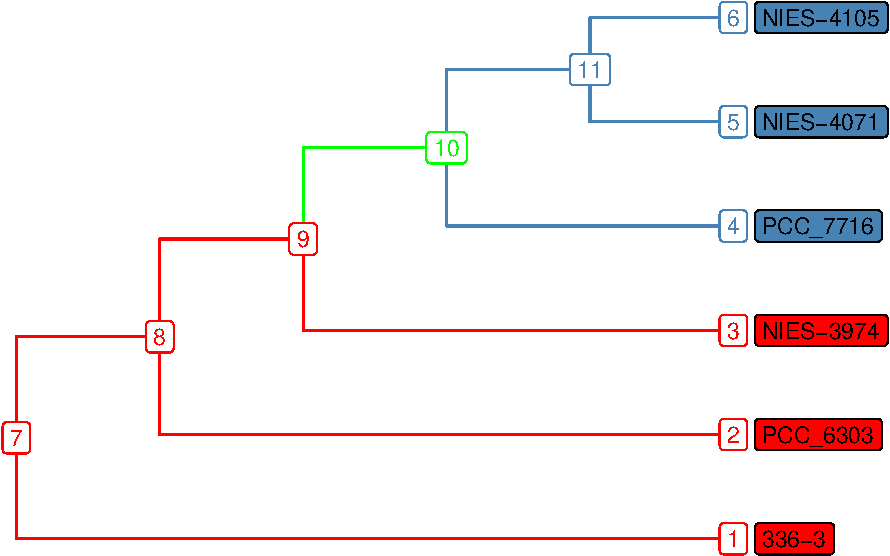
\includegraphics{ResultadosII_files/figure-latex/FIG15-1.pdf}
\caption{\label{fig:FIG15}\textbf{Filogenia del clado Calotrix}. En rojo y azul se muestran los subclados unidos (en verde) por la transición entre los nodos 9 y 10.}
\end{figure}

Para hacer esto filtramos los datos de la red para mostrar unicamente las transiciones que se dieron entre los nodos 9 y 10 e hicimos las mismas figuras.
En la (Figura \ref{fig:FIG16}) se muestra la red como una conexión de nodos a través de vertices con un grosor proporcional al numero de veces que ocurrió cada transición. En la (Figura \ref{fig:FIG17}) podemos ver las transiciones de una forma mas ordenada, con el numero de ocurrencias y la dirección en la que ocurrieron.

\hypertarget{mutaciones-en-los-codones}{%
\subsubsection{Mutaciones en los codones}\label{mutaciones-en-los-codones}}

Para entender como es que se van ganando o perdiendo los sitios palindrómicos hicimos un análisis del tipo mutaciones de los sitios. Esto lo hicimos viendo en que marco de lectura se encontraba cada nodo y revisando la secuencia de aminoacidos que codificaban. En la (Figura \ref{fig:FIG18}) mostramos 3 gráficos que indican la abundancia de los peptidos codificados por los sitios palindrómicos de acuerdo al marco de lectura en el que se encuentran. En esta figura podemos observar que el marco de lectura es el que contiene la mayoria de los sitios

\begin{figure}

{\centering 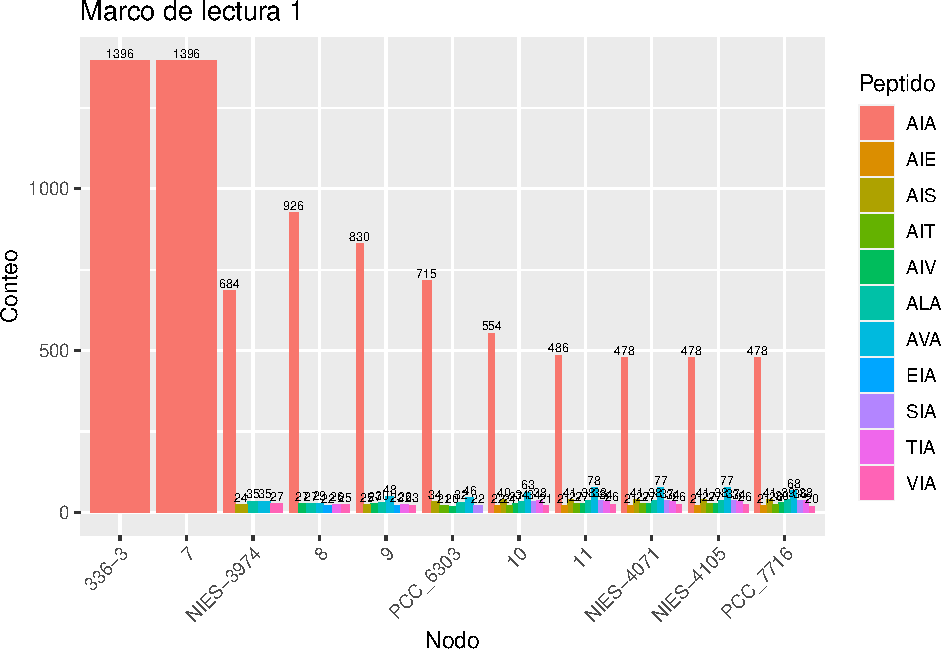
\includegraphics[width=1.1\linewidth]{ResultadosII_files/figure-latex/FIG18-1} 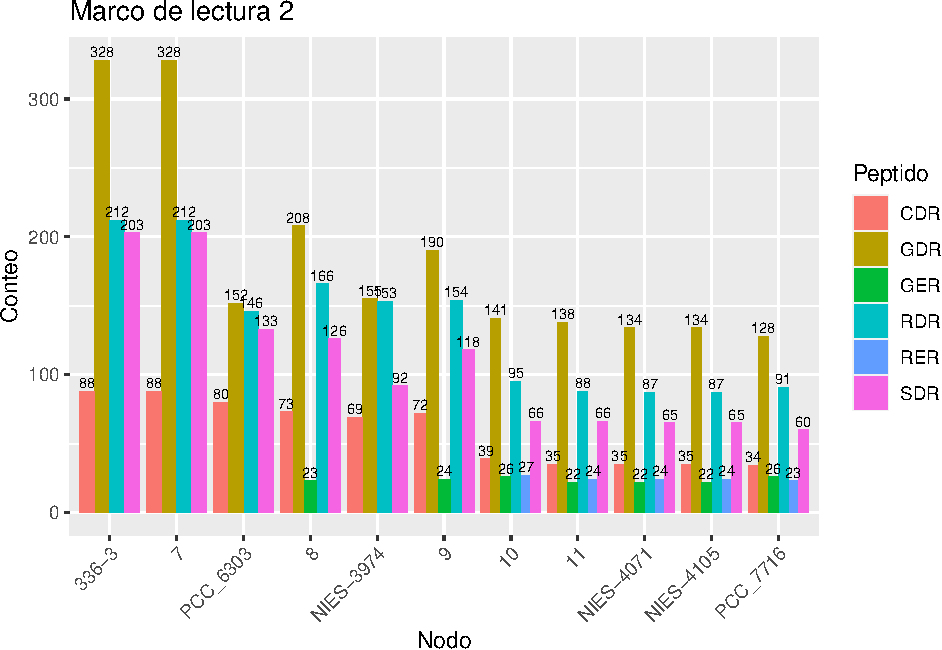
\includegraphics[width=1.1\linewidth]{ResultadosII_files/figure-latex/FIG18-2} 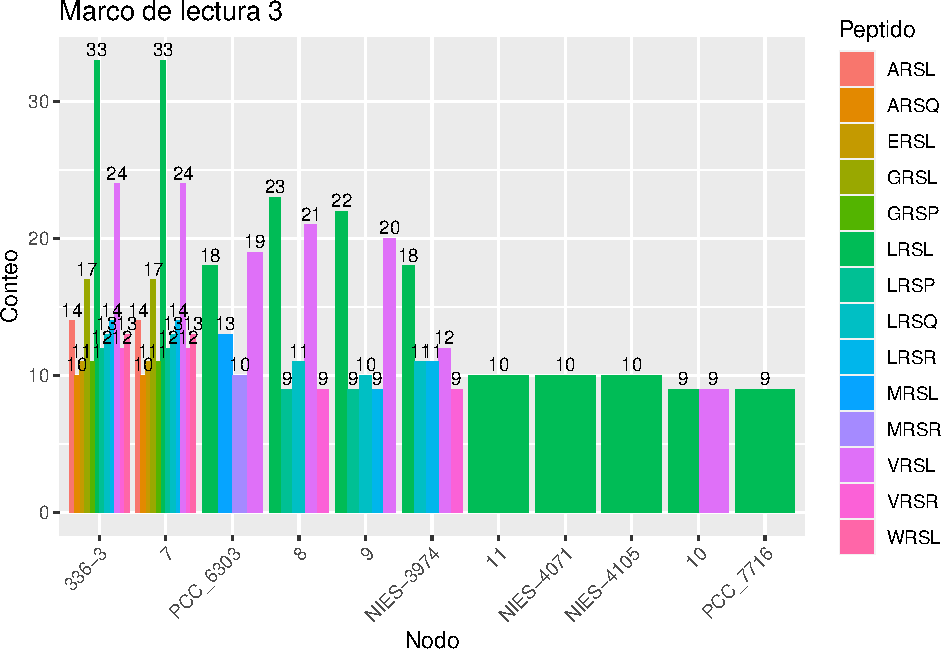
\includegraphics[width=1.1\linewidth]{ResultadosII_files/figure-latex/FIG18-3} 

}

\caption{**Abundancia de peptidos por cada nodo segun el marco de lectura.**.}\label{fig:FIG18}
\end{figure}

En la (Figura \ref{fig:FIG19}) mostramos 3 gráficos que indican la abundancia del tipo de mutaciones que hay en cada nodo de acuerdo al marco de lectura. Lo sitios de mutaciones mostrados pueden ser de los siguientes tipos:

\begin{itemize}
\tightlist
\item
  Conservative (la secuencia de AA cambió pero tiene similitud de acuerdo al score de BLOSUM62)
\item
  ConservativeNoSiteMut (la secuencia de AA cambió pero tiene similitud de acuerdo al score de BLOSUM62. Sin embargo, el sitio no sufrió mutaciones)
\item
  Deletion (La secuencia de AA tiene sufrio 1 o mas deleciones)
\item
  NoMutation (La secuencia de AA no sufrio mutaciones)
\item
  NoSynonym (La secuencia de AA cambió)
\item
  NoSynonymNoSiteMut (La secuencia de AA cambió. Sin embargo, el sitio no sufrió mutaciones.)
\item
  Synonym (El sitio sufrió mutaciones. Sin embargo, la secuencia de AA no cambió.)
\end{itemize}

\begin{figure}

{\centering 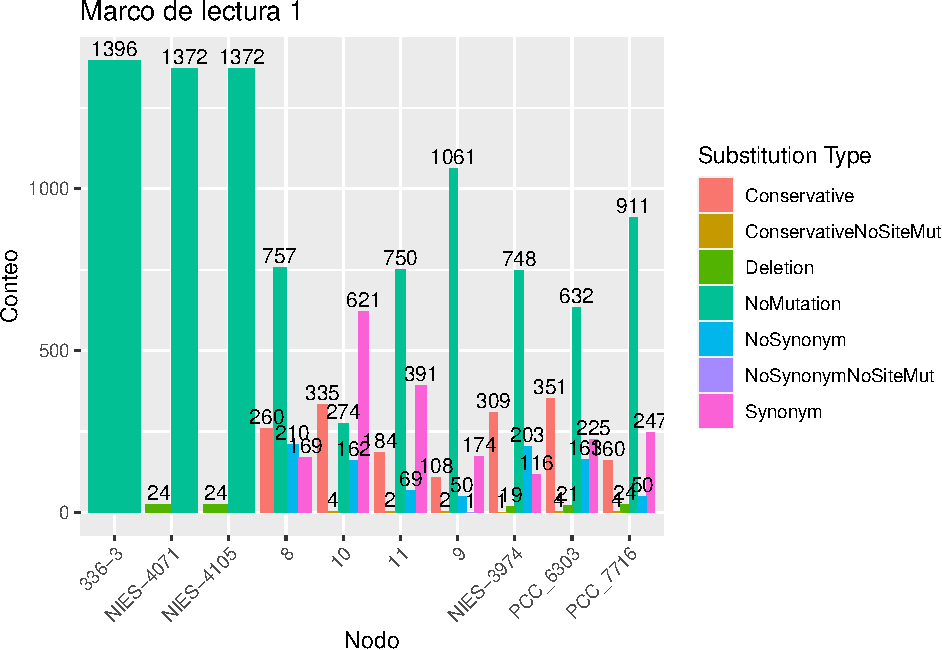
\includegraphics[width=1.1\linewidth]{ResultadosII_files/figure-latex/FIG19-1} 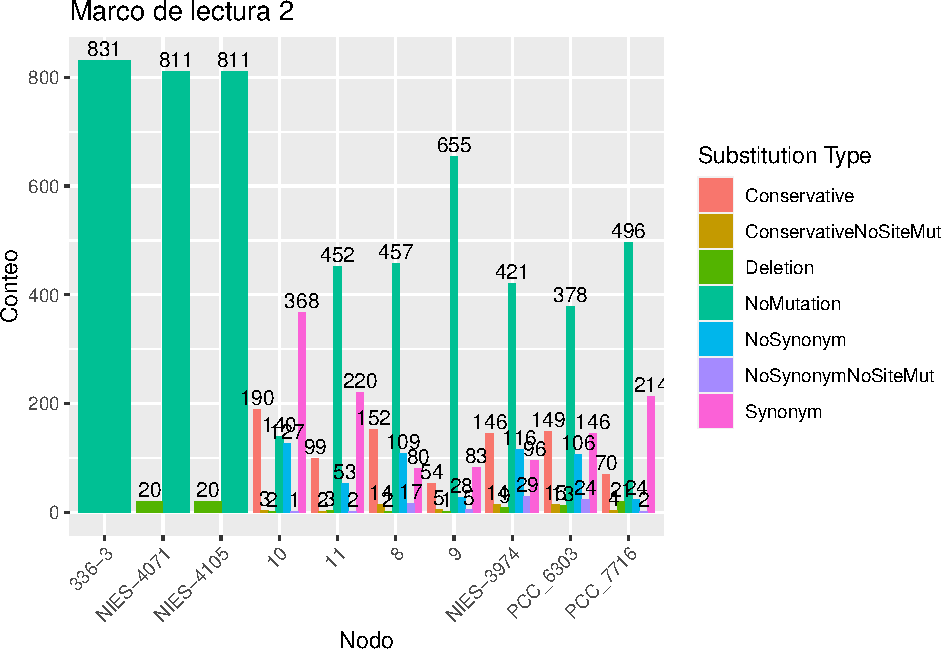
\includegraphics[width=1.1\linewidth]{ResultadosII_files/figure-latex/FIG19-2} 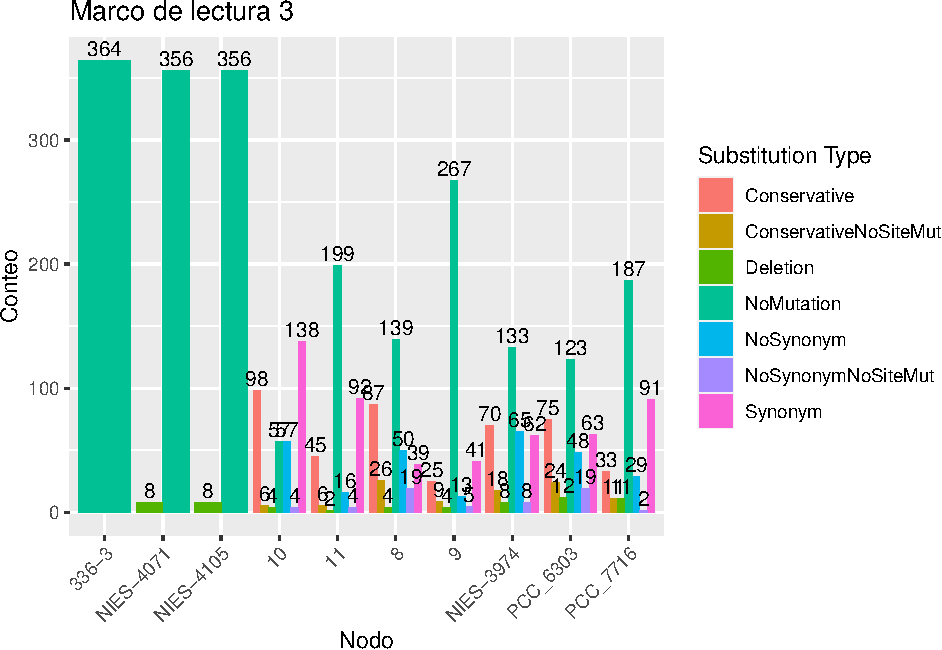
\includegraphics[width=1.1\linewidth]{ResultadosII_files/figure-latex/FIG19-3} 

}

\caption{**Abundancia del tipo de sustitución por cada nodo segun el marco de lectura.**.}\label{fig:FIG19}
\end{figure}

\hypertarget{anuxe1lisis-de-sitios-en-los-cuales-su-ancestro-era-hip1}{%
\subsubsection{Análisis de sitios en los cuales su ancestro era HIP1}\label{anuxe1lisis-de-sitios-en-los-cuales-su-ancestro-era-hip1}}

Para tratar de entender como es que los sitios HIP1 se pierden hicimos un análisis unicamente en en las transiciones en las que el nodo ancestral tenia un sitio HIP1.

En la (Figura \ref{fig:FIG20}) mostramos 3 gráficos que indican la frecuencia del tipo de sustituciones que hubo para estos casos para cada nodo en cada uno de los marcos de lectura.

\begin{figure}

{\centering 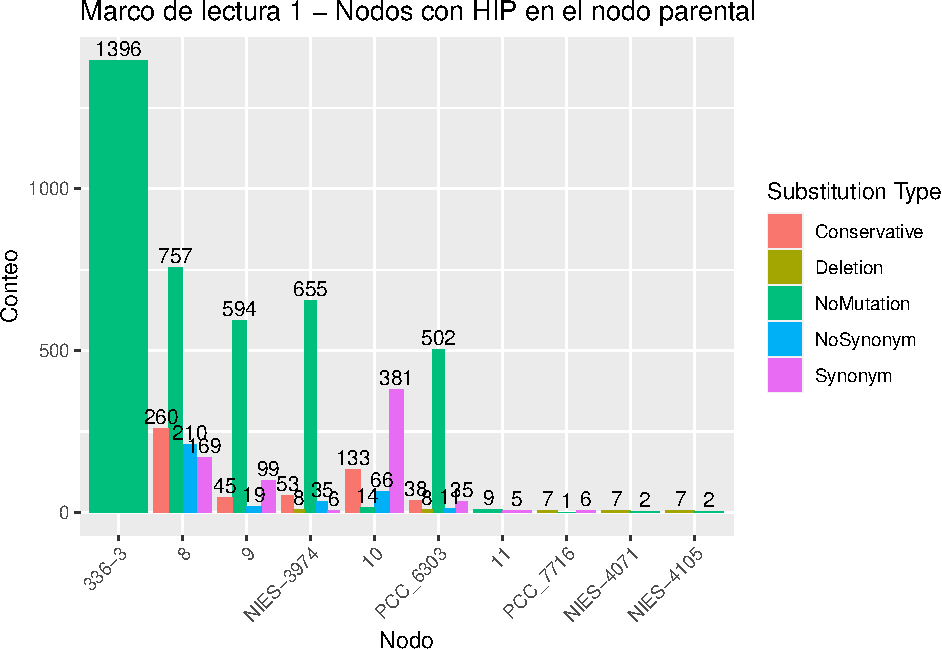
\includegraphics[width=1.1\linewidth]{ResultadosII_files/figure-latex/FIG20-1} 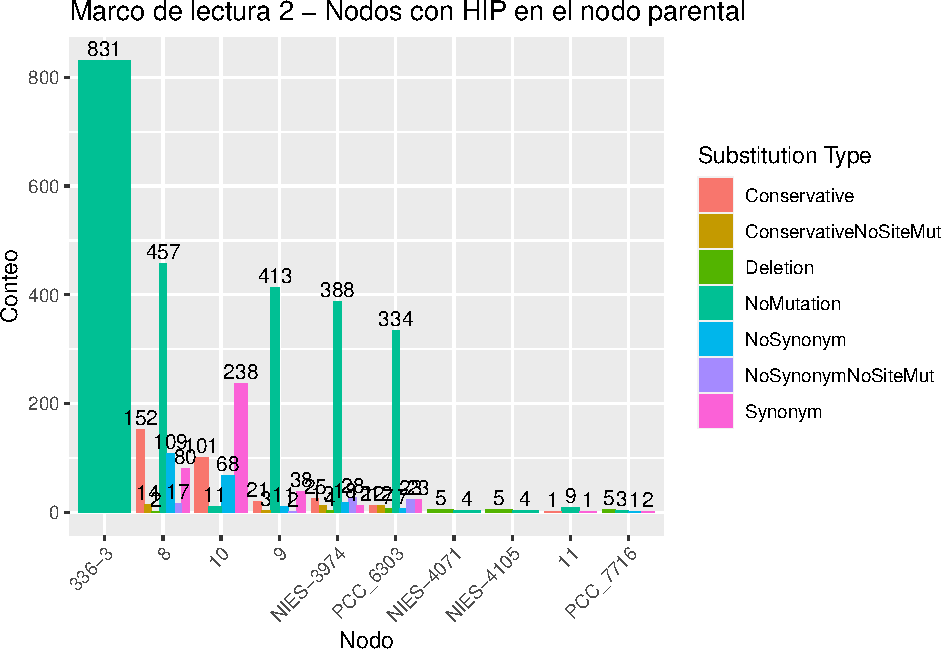
\includegraphics[width=1.1\linewidth]{ResultadosII_files/figure-latex/FIG20-2} 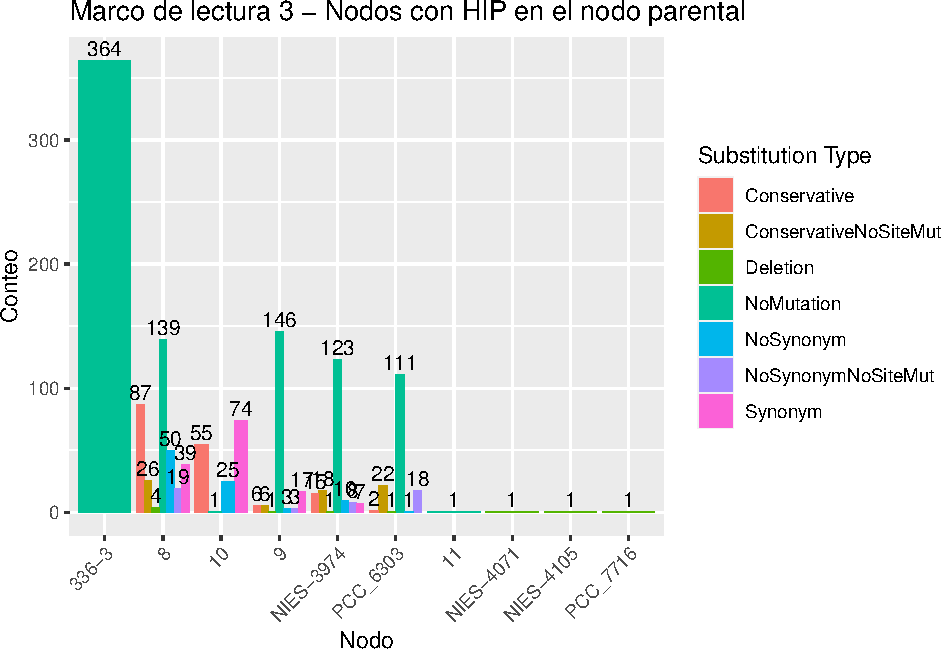
\includegraphics[width=1.1\linewidth]{ResultadosII_files/figure-latex/FIG20-3} 

}

\caption{**Abundancia del tipo de sustitución por cada nodo segun el marco de lectura. Unicamente para transiciones en los que el nodo ancestral era un sitio HIP1.**}\label{fig:FIG20}
\end{figure}

En la (Figura \ref{fig:FIG21}) mostramos 3 gráficos (uno por cada marco de lectura) que indican la frecuencia de las mutaciones en cada uno de los 8 nucleótidos del sitio HIP.

\begin{figure}

{\centering 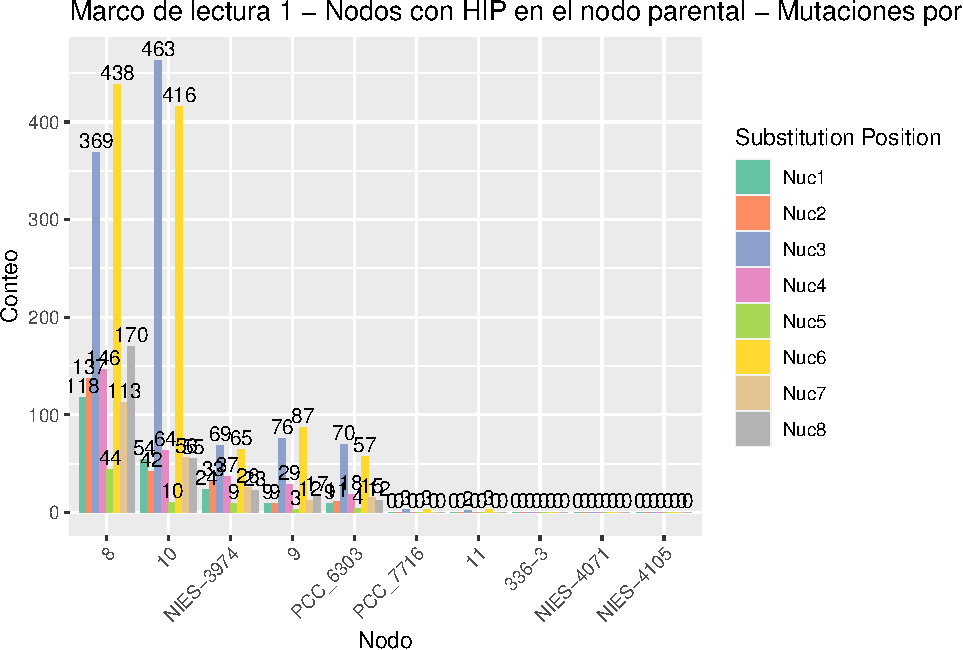
\includegraphics[width=1.1\linewidth]{ResultadosII_files/figure-latex/FIG21-1} 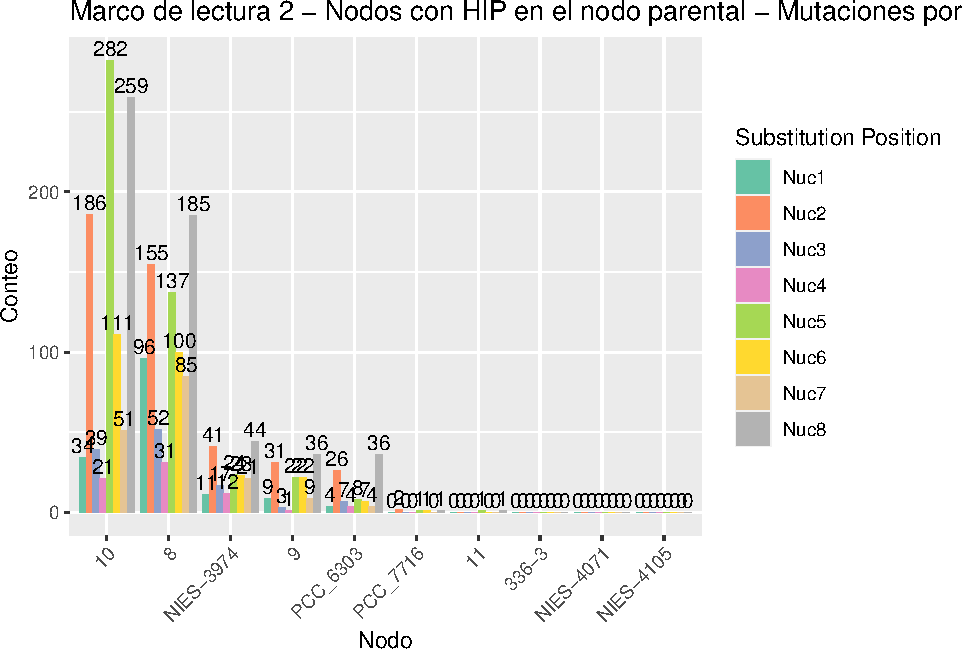
\includegraphics[width=1.1\linewidth]{ResultadosII_files/figure-latex/FIG21-2} 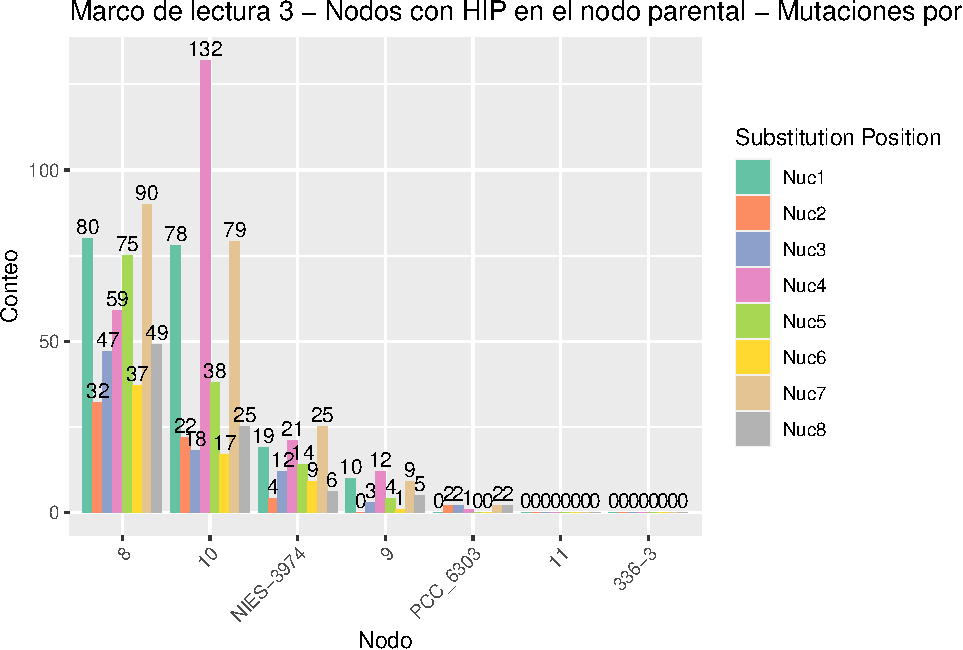
\includegraphics[width=1.1\linewidth]{ResultadosII_files/figure-latex/FIG21-3} 

}

\caption{**Frecuencia de las mutaciones de cada nucleótido del sitio HIP para cada nodo segun el marco de lectura.**.}\label{fig:FIG21}
\end{figure}

En la (Figura \ref{fig:FIG22}) mostramos 3 gráficos (uno por cada marco de lectura) que indican la frecuencia del tipo sustitucion de bases.

\begin{figure}

{\centering 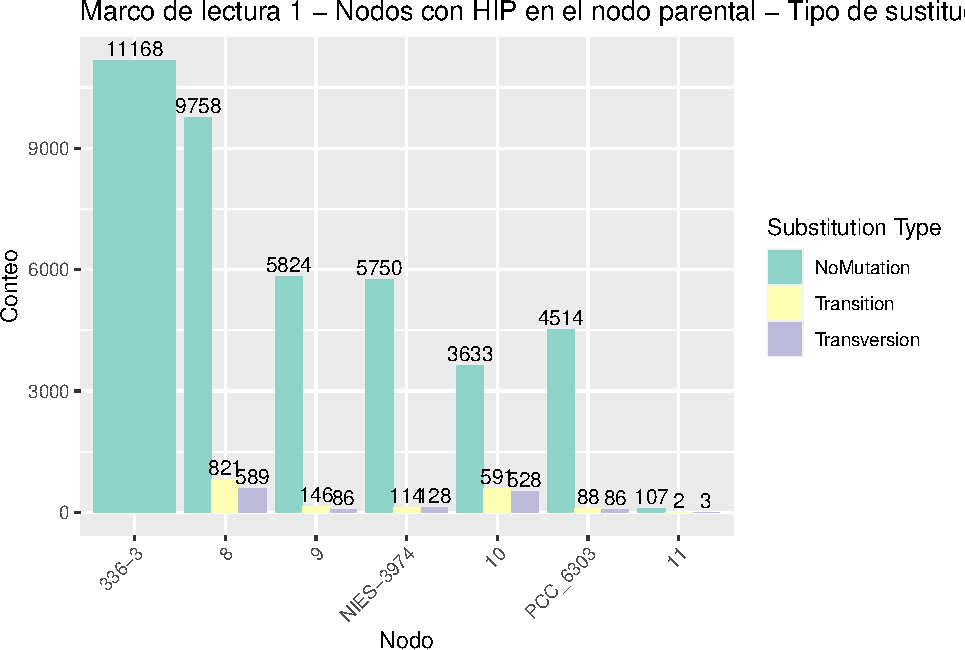
\includegraphics[width=1.1\linewidth]{ResultadosII_files/figure-latex/FIG22-1} 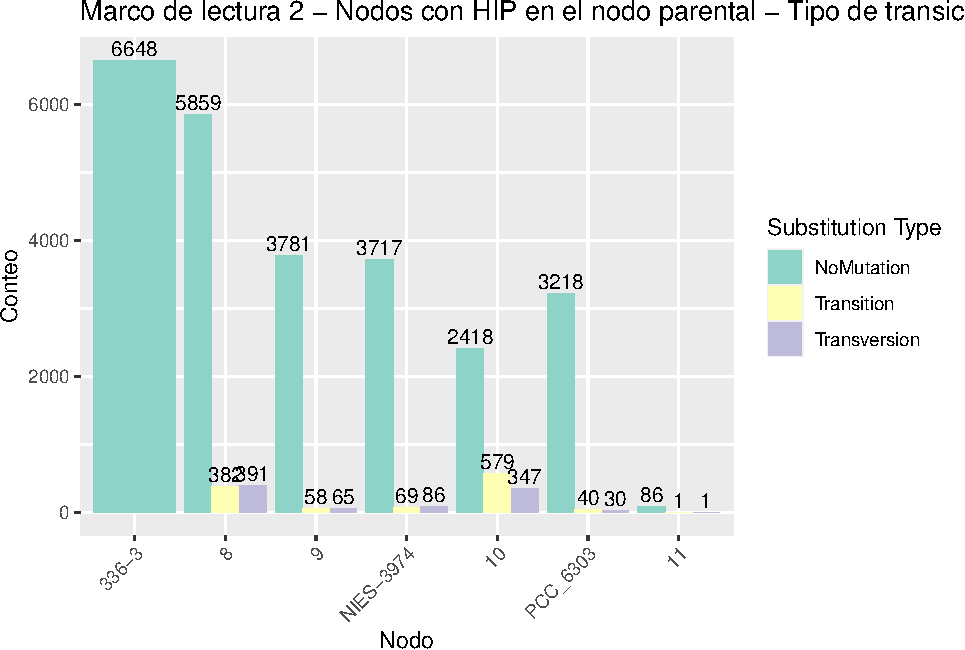
\includegraphics[width=1.1\linewidth]{ResultadosII_files/figure-latex/FIG22-2} 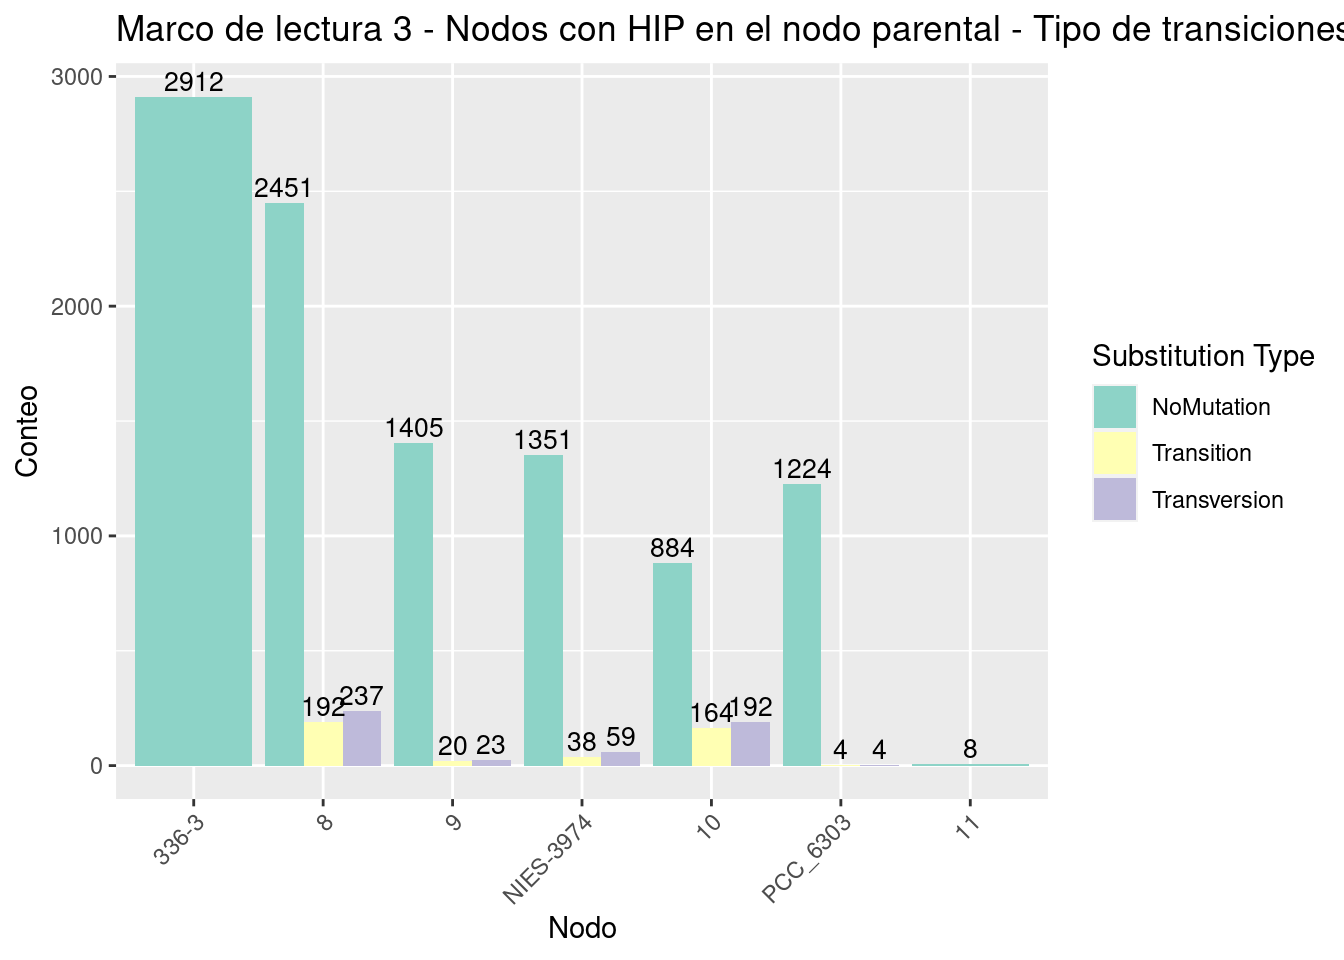
\includegraphics[width=1.1\linewidth]{ResultadosII_files/figure-latex/FIG22-3} 

}

\caption{**Frecuencia del tipo de sustituciónes de base en los sitios HIP para cada marco de lectura**.}\label{fig:FIG22}
\end{figure}

\hypertarget{anuxe1lisis-de-sitios-en-los-cuales-solo-el-nodo-actual-tiene-hip1}{%
\subsubsection{Análisis de sitios en los cuales solo el nodo actual tiene HIP1}\label{anuxe1lisis-de-sitios-en-los-cuales-solo-el-nodo-actual-tiene-hip1}}

Para tratar de entender como es que los sitios HIP se ganan, hicimos un analisis unicamente en las transiciones en las que el nodo actual tenia un sitio HIP1.

En la Figura \ref{fig:FIG23} mostramos 3 gráficos (uno por cada marco de lectura) que indican la frecuencia del tipo de sustituciones que hubo para estos casos para cada nodo en cada uno de los marcos de lectura.

\begin{figure}

{\centering 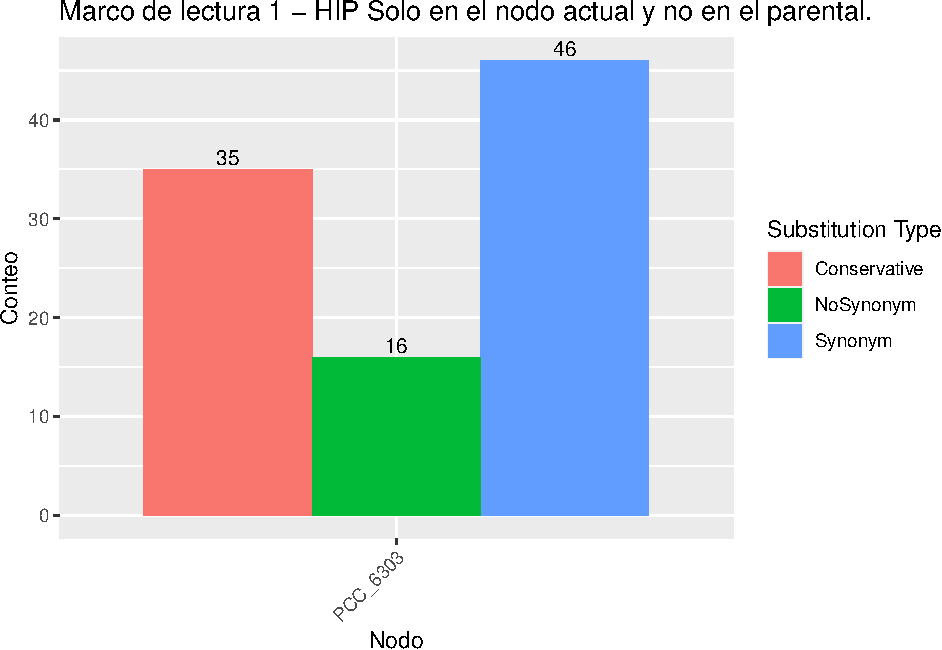
\includegraphics[width=1.1\linewidth]{ResultadosII_files/figure-latex/FIG23-1} 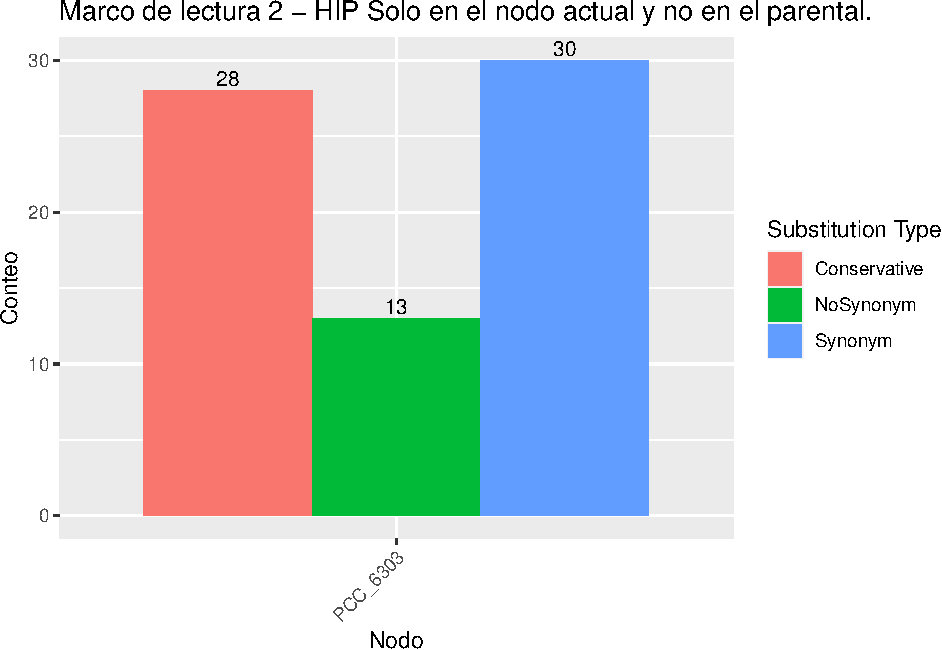
\includegraphics[width=1.1\linewidth]{ResultadosII_files/figure-latex/FIG23-2} 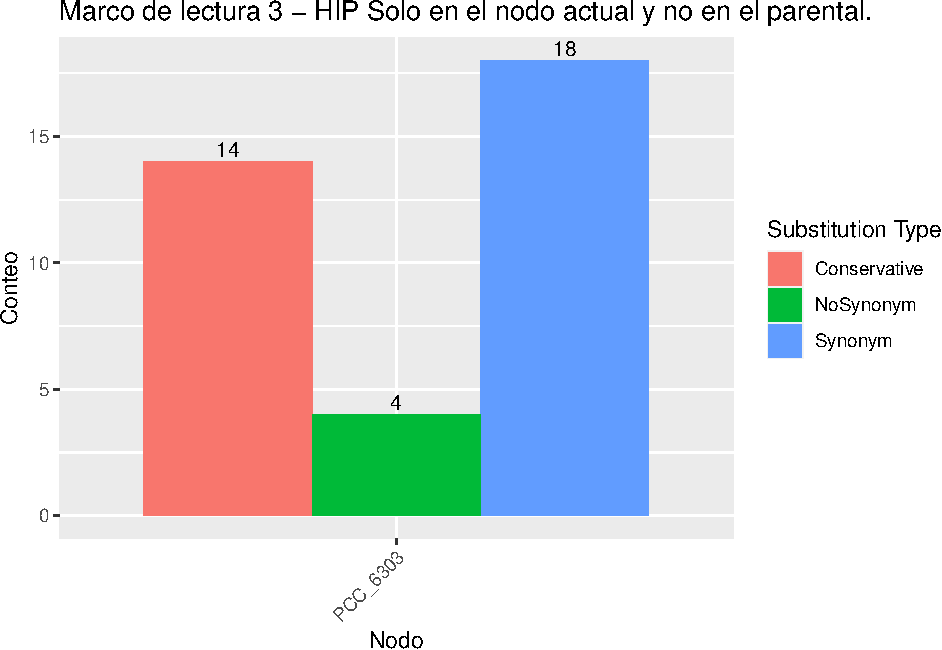
\includegraphics[width=1.1\linewidth]{ResultadosII_files/figure-latex/FIG23-3} 

}

\caption{**Abundancia del tipo de sustitución por cada nodo segun el marco de lectura. Unicamente para transiciones en los que el nodo actual era un sitio HIP1.**.}\label{fig:FIG23}
\end{figure}

\hypertarget{conjunto-de-sitios-hip1-usando-la-especie-nies-3974-como-referencia}{%
\subsection{Conjunto de sitios HIP1 usando la especie NIES-3974 como referencia}\label{conjunto-de-sitios-hip1-usando-la-especie-nies-3974-como-referencia}}

\hypertarget{red-de-transiciones-1}{%
\subsubsection{Red de transiciones}\label{red-de-transiciones-1}}

visualizamos dicha red .

Para visualizar la red usamos la paqueteria \texttt{networkD3}. Hicimos 2 figuras, la (Figura \ref{fig:FIG44}) muestra la red como una conexión de nodos a través de vertices con un grosor proporcional al numero de veces que ocurrió cada transición.

En la (Figura \ref{fig:FIG45}) podemos ver las transiciones de una forma mas ordenada, con el numero de ocurrencias y la dirección en la que ocurrieron.

\hypertarget{transiciones-entre-nodo-9-y-nodo-10-1}{%
\subsubsection{Transiciones entre Nodo 9 y Nodo 10}\label{transiciones-entre-nodo-9-y-nodo-10-1}}

Para entender más como es que se gana o se pierden los sitios palindrómicos revisamos la transición en tre los nodos 9 y 10. Esto es porque es esta transicion de nodos la que separa a los dos subclados entre los que hay una repentino cambio de abundancia de sitios palindrómicos (Figura \ref{fig:FIG15}).

Para hacer esto filtramos los datos de la red para mostrar unicamente las transiciones que se dieron entre los nodos 9 y 10 e hicimos las mismas figuras.
En la (Figura \ref{fig:FIG46}) se muestra la red como una conexión de nodos a través de vertices con un grosor proporcional al numero de veces que ocurrió cada transición. En la (Figura \ref{fig:FIG47}) podemos ver las transiciones de una forma mas ordenada, con el numero de ocurrencias y la dirección en la que ocurrieron.

\hypertarget{mutaciones-en-los-codones-1}{%
\subsubsection{Mutaciones en los codones}\label{mutaciones-en-los-codones-1}}

Para entender como es que se van ganando o perdiendo los sitios palindrómicos hicimos un análisis del tipo mutaciones de los sitios. Esto lo hicimos viendo en que marco de lectura se encontraba cada nodo y revisando la secuencia de aminoacidos que codificaban. En la (Figura \ref{fig:FIG48}) mostramos 3 gráficos que indican la abundancia de los peptidos codificados por los sitios palindrómicos de acuerdo al marco de lectura en el que se encuentran. En esta figura podemos observar que el marco de lectura es el que contiene la mayoria de los sitios

\begin{figure}

{\centering 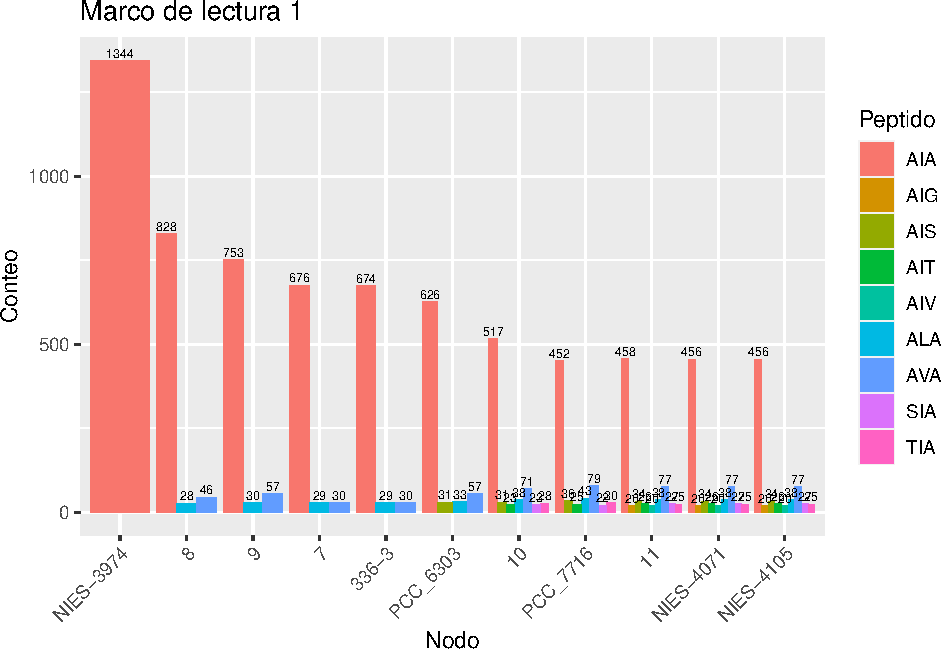
\includegraphics[width=1.1\linewidth]{ResultadosII_files/figure-latex/FIG48-1} 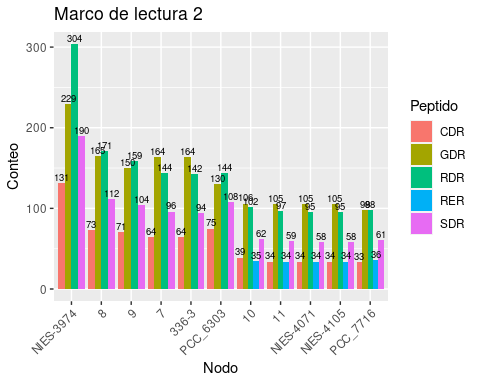
\includegraphics[width=1.1\linewidth]{ResultadosII_files/figure-latex/FIG48-2} 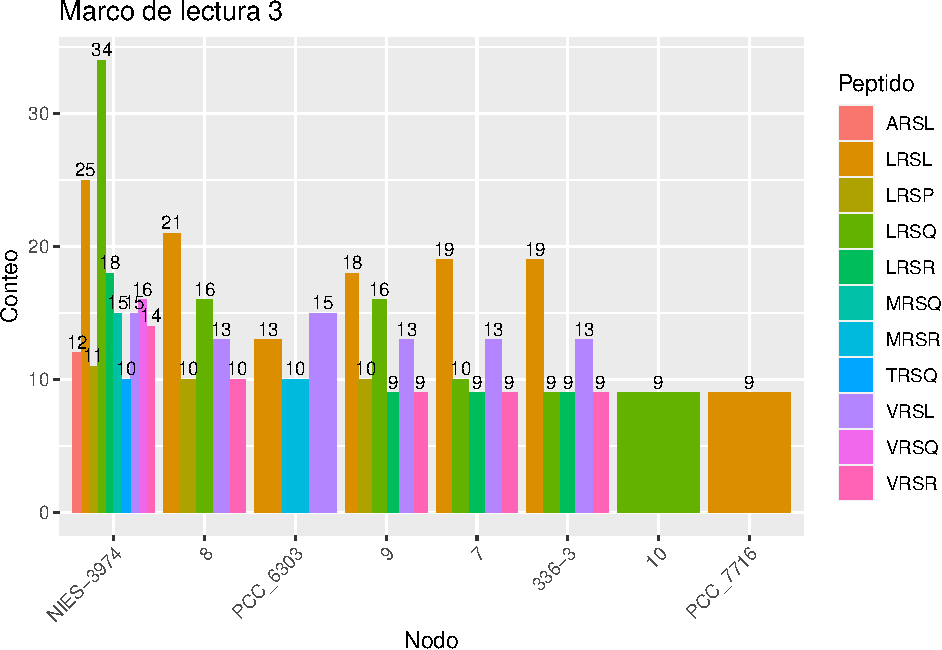
\includegraphics[width=1.1\linewidth]{ResultadosII_files/figure-latex/FIG48-3} 

}

\caption{**Abundancia de peptidos por cada nodo segun el marco de lectura.**.}\label{fig:FIG48}
\end{figure}

En la (Figura \ref{fig:FIG49}) mostramos 3 gráficos que indican la abundancia del tipo de mutaciones que hay en cada nodo de acuerdo al marco de lectura. Lo sitios de mutaciones mostrados pueden ser de los siguientes tipos:

\begin{itemize}
\tightlist
\item
  Conservative (la secuencia de AA cambió pero tiene similitud de acuerdo al score de BLOSUM62)
\item
  ConservativeNoSiteMut (la secuencia de AA cambió pero tiene similitud de acuerdo al score de BLOSUM62. Sin embargo, el sitio no sufrió mutaciones)
\item
  Deletion (La secuencia de AA tiene sufrio 1 o mas deleciones)
\item
  NoMutation (La secuencia de AA no sufrio mutaciones)
\item
  NoSynonym (La secuencia de AA cambió)
\item
  NoSynonymNoSiteMut (La secuencia de AA cambió. Sin embargo, el sitio no sufrió mutaciones.)
\item
  Synonym (El sitio sufrió mutaciones. Sin embargo, la secuencia de AA no cambió.)
\end{itemize}

\begin{figure}

{\centering 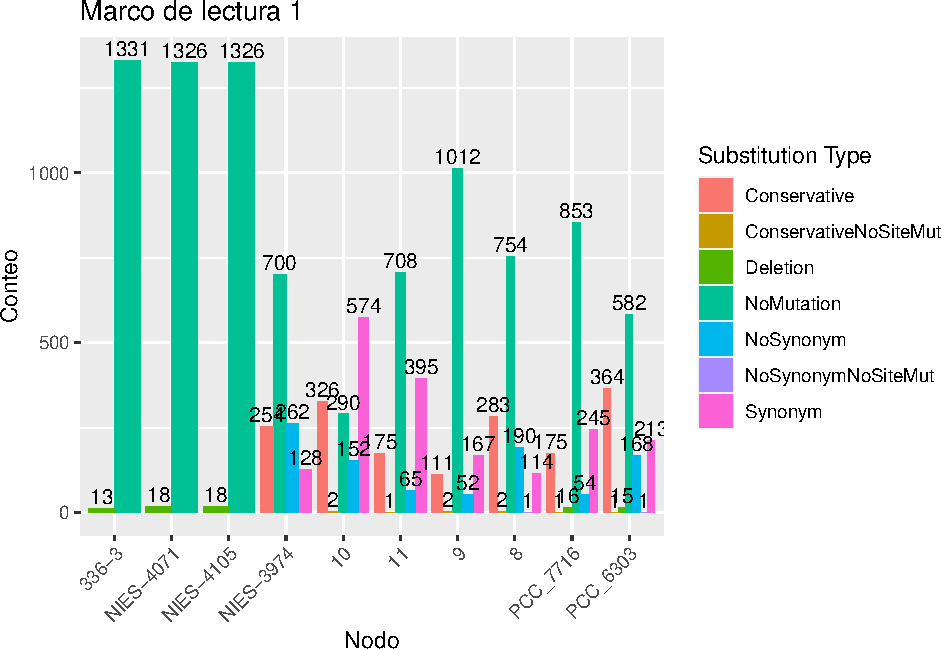
\includegraphics[width=1.1\linewidth]{ResultadosII_files/figure-latex/FIG49-1} 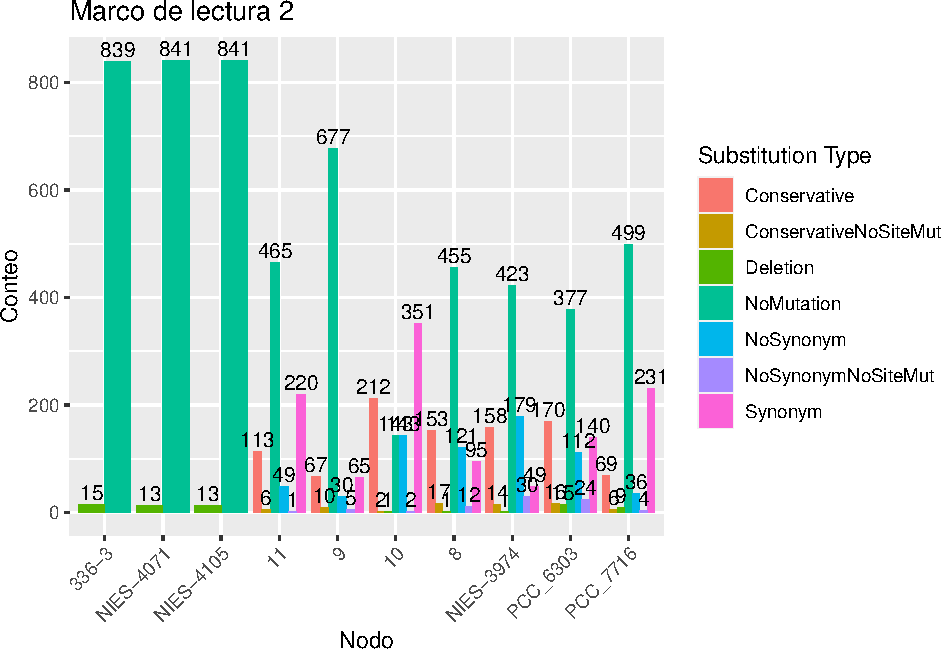
\includegraphics[width=1.1\linewidth]{ResultadosII_files/figure-latex/FIG49-2} 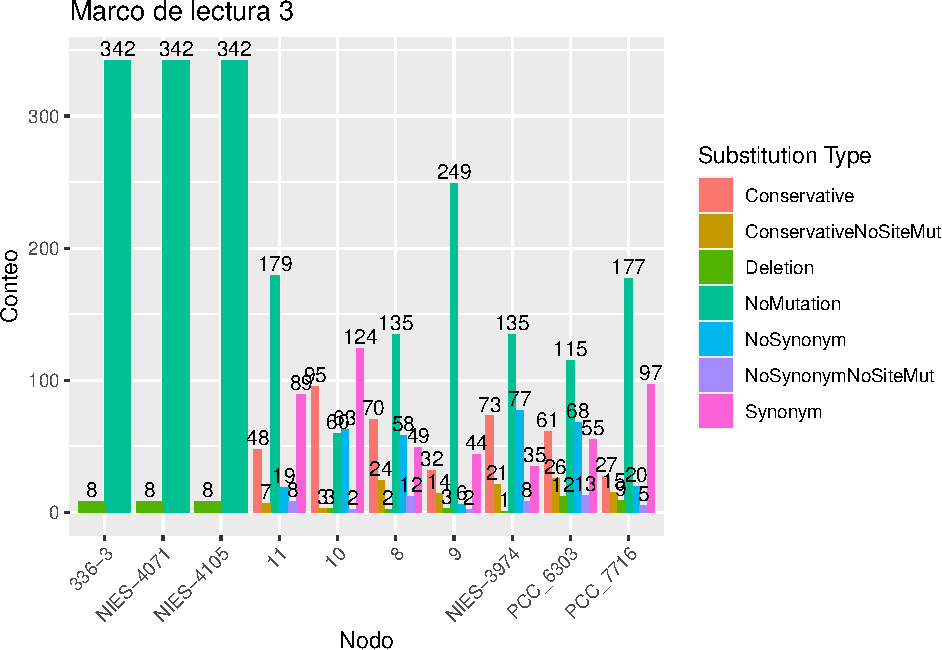
\includegraphics[width=1.1\linewidth]{ResultadosII_files/figure-latex/FIG49-3} 

}

\caption{**Abundancia del tipo de sustitución por cada nodo segun el marco de lectura.**.}\label{fig:FIG49}
\end{figure}

\hypertarget{anuxe1lisis-de-sitios-en-los-cuales-su-ancestro-era-hip1-1}{%
\subsubsection{Análisis de sitios en los cuales su ancestro era HIP1}\label{anuxe1lisis-de-sitios-en-los-cuales-su-ancestro-era-hip1-1}}

Para tratar de entender como es que los sitios HIP1 se pierden hicimos un análisis unicamente en en las transiciones en las que el nodo ancestral tenia un sitio HIP1.

En la (Figura \ref{fig:FIG50}) mostramos 3 gráficos que indican la frecuencia del tipo de sustituciones que hubo para estos casos para cada nodo en cada uno de los marcos de lectura.

\begin{figure}

{\centering 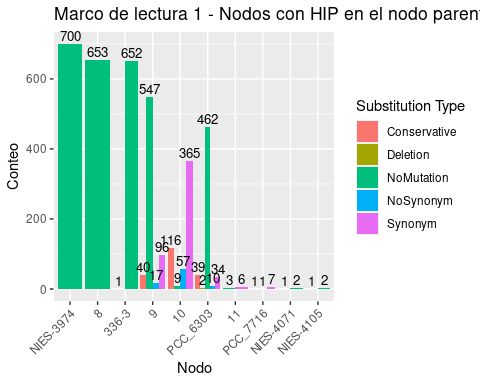
\includegraphics[width=1.1\linewidth]{ResultadosII_files/figure-latex/FIG50-1} 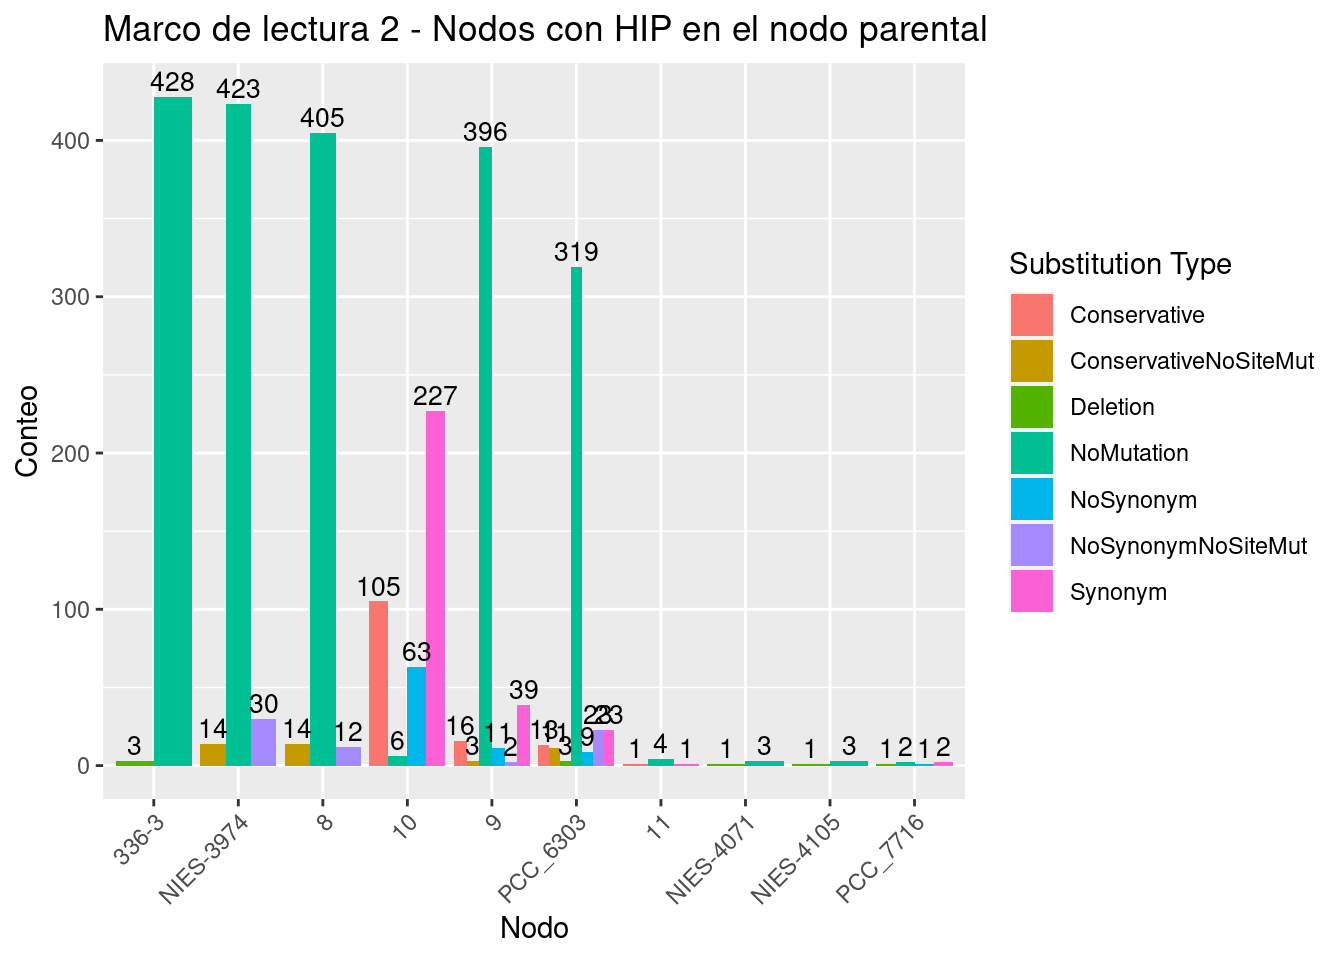
\includegraphics[width=1.1\linewidth]{ResultadosII_files/figure-latex/FIG50-2} 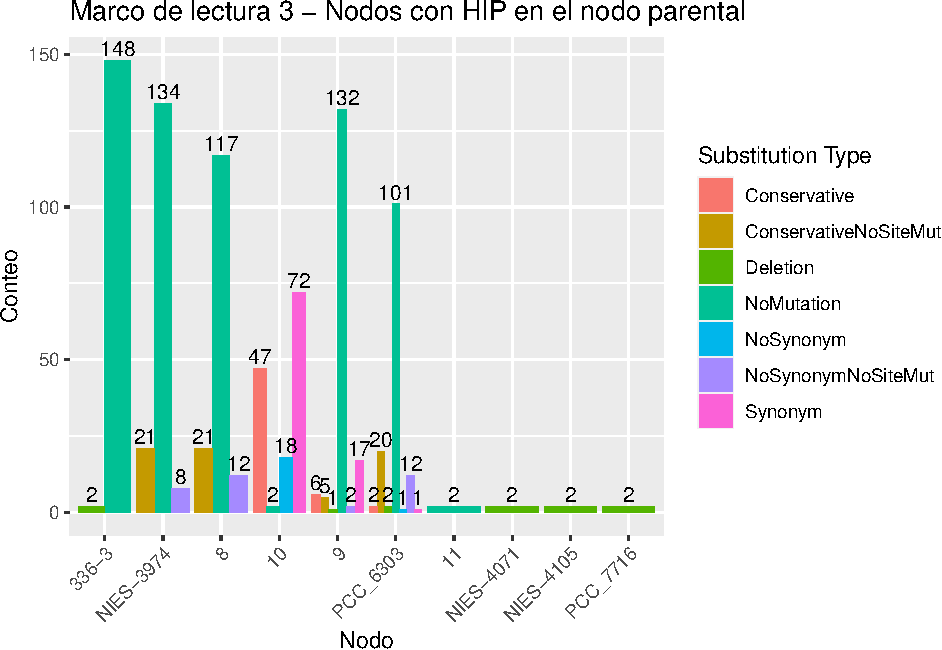
\includegraphics[width=1.1\linewidth]{ResultadosII_files/figure-latex/FIG50-3} 

}

\caption{**Abundancia del tipo de sustitución por cada nodo segun el marco de lectura. Unicamente para transiciones en los que el nodo ancestral era un sitio HIP1.**}\label{fig:FIG50}
\end{figure}

En la (Figura \ref{fig:FIG51}) mostramos 3 gráficos (uno por cada marco de lectura) que indican la frecuencia de las mutaciones en cada uno de los 8 nucleótidos del sitio HIP.

\begin{figure}

{\centering 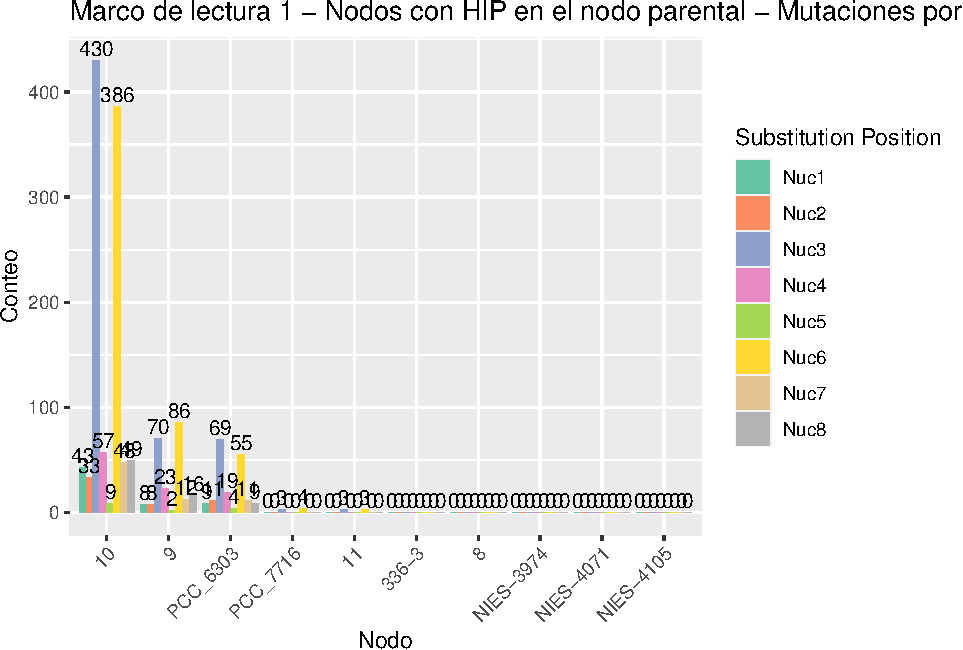
\includegraphics[width=1.1\linewidth]{ResultadosII_files/figure-latex/FIG51-1} 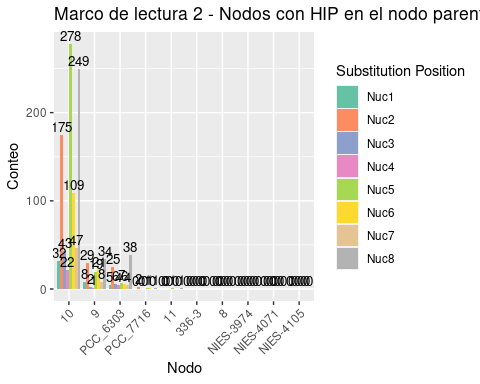
\includegraphics[width=1.1\linewidth]{ResultadosII_files/figure-latex/FIG51-2} 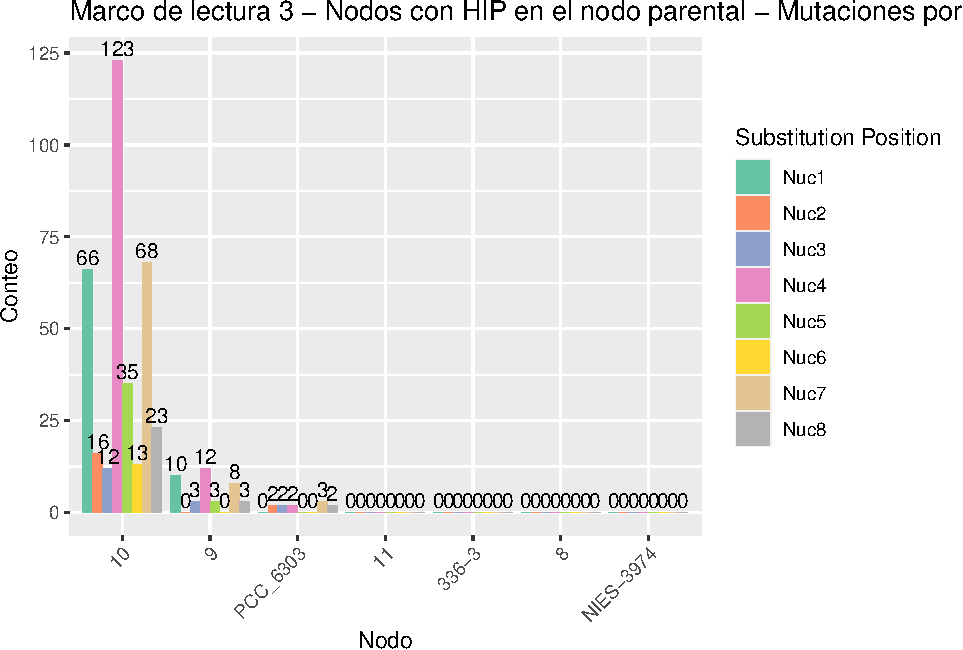
\includegraphics[width=1.1\linewidth]{ResultadosII_files/figure-latex/FIG51-3} 

}

\caption{**Frecuencia de las mutaciones de cada nucleótido del sitio HIP para cada nodo segun el marco de lectura.**.}\label{fig:FIG51}
\end{figure}

En la (Figura \ref{fig:FIG52}) mostramos 3 gráficos (uno por cada marco de lectura) que indican la frecuencia del tipo sustitucion de bases.

\begin{figure}

{\centering 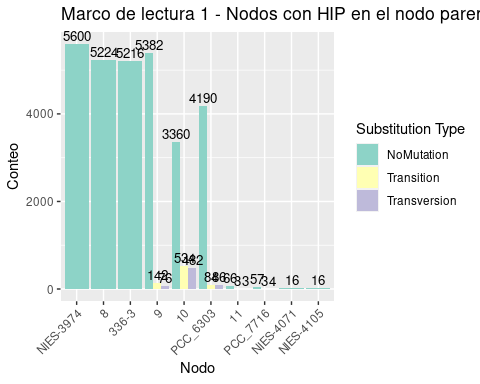
\includegraphics[width=1.1\linewidth]{ResultadosII_files/figure-latex/FIG52-1} 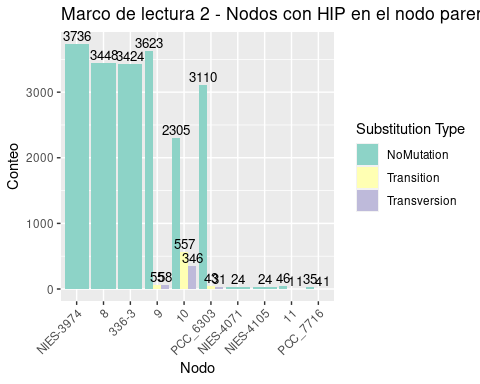
\includegraphics[width=1.1\linewidth]{ResultadosII_files/figure-latex/FIG52-2} 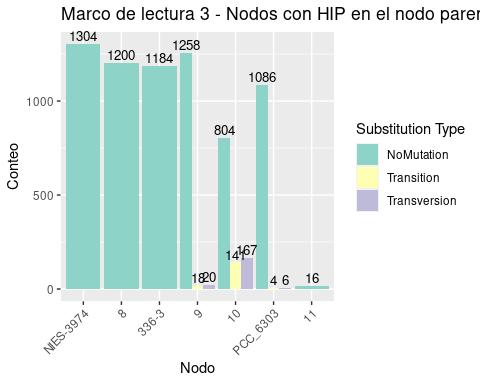
\includegraphics[width=1.1\linewidth]{ResultadosII_files/figure-latex/FIG52-3} 

}

\caption{**Frecuencia del tipo de sustituciónes de base en los sitios HIP para cada marco de lectura**.}\label{fig:FIG52}
\end{figure}

\hypertarget{anuxe1lisis-de-sitios-en-los-cuales-solo-el-nodo-actual-tiene-hip1-1}{%
\subsubsection{Análisis de sitios en los cuales solo el nodo actual tiene HIP1}\label{anuxe1lisis-de-sitios-en-los-cuales-solo-el-nodo-actual-tiene-hip1-1}}

Para tratar de entender como es que los sitios HIP se ganan, hicimos un analisis unicamente en las transiciones en las que el nodo actual tenia un sitio HIP1.

En la Figura \ref{fig:FIG53} mostramos 3 gráficos (uno por cada marco de lectura) que indican la frecuencia del tipo de sustituciones que hubo para estos casos para cada nodo en cada uno de los marcos de lectura.

\begin{figure}

{\centering 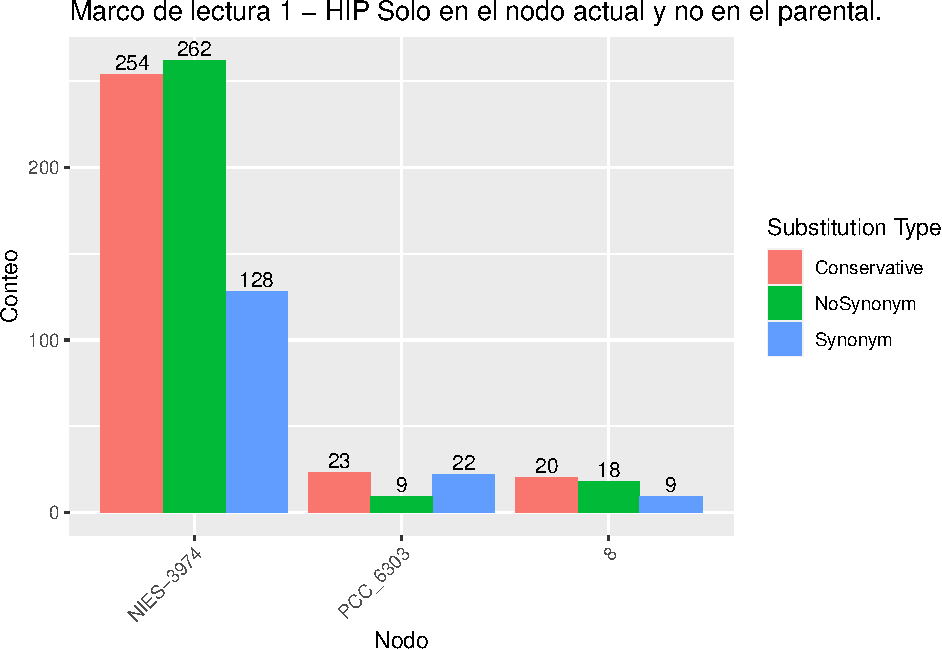
\includegraphics[width=1.1\linewidth]{ResultadosII_files/figure-latex/FIG53-1} 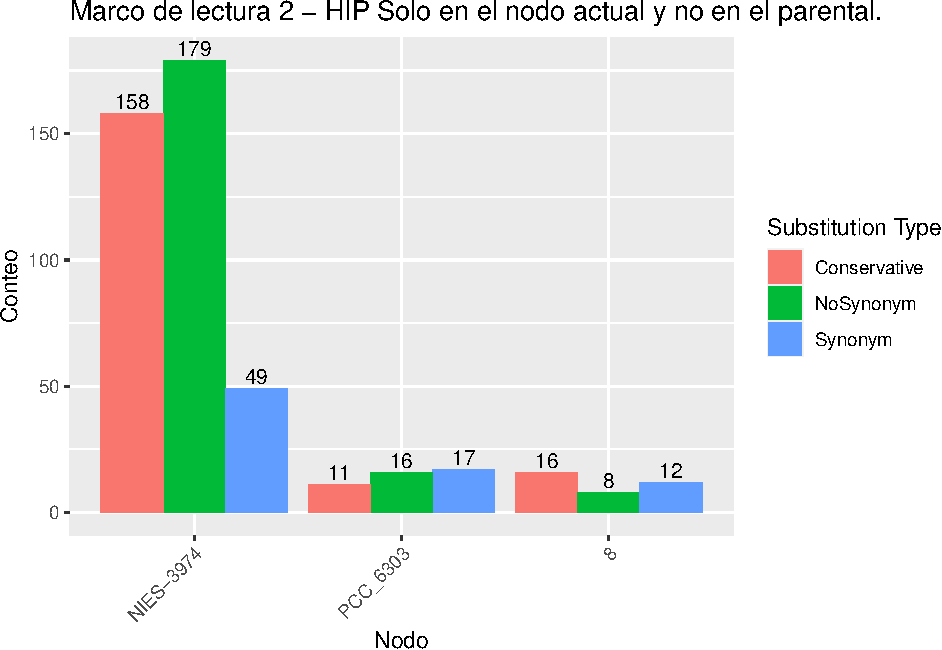
\includegraphics[width=1.1\linewidth]{ResultadosII_files/figure-latex/FIG53-2} 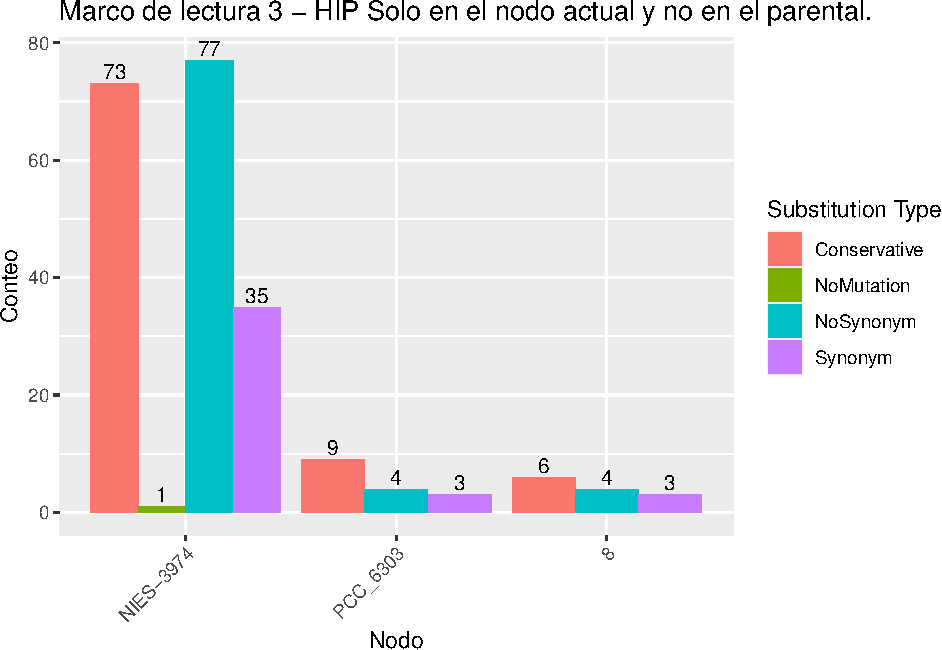
\includegraphics[width=1.1\linewidth]{ResultadosII_files/figure-latex/FIG53-3} 

}

\caption{**Abundancia del tipo de sustitución por cada nodo segun el marco de lectura. Unicamente para transiciones en los que el nodo actual era un sitio HIP1.**.}\label{fig:FIG53}
\end{figure}

\hypertarget{conjunto-de-sitios-hip1-usando-la-especie-pcc_6303-como-referencia}{%
\subsection{Conjunto de sitios HIP1 usando la especie PCC\_6303 como referencia}\label{conjunto-de-sitios-hip1-usando-la-especie-pcc_6303-como-referencia}}

\hypertarget{red-de-transiciones-2}{%
\subsubsection{Red de transiciones}\label{red-de-transiciones-2}}

visualizamos dicha red .

Para visualizar la red usamos la paqueteria \texttt{networkD3}. Hicimos 2 figuras, la (Figura \ref{fig:FIG54}) muestra la red como una conexión de nodos a través de vertices con un grosor proporcional al numero de veces que ocurrió cada transición.

En la (Figura \ref{fig:FIG55}) podemos ver las transiciones de una forma mas ordenada, con el numero de ocurrencias y la dirección en la que ocurrieron.

\hypertarget{transiciones-entre-nodo-9-y-nodo-10-2}{%
\subsubsection{Transiciones entre Nodo 9 y Nodo 10}\label{transiciones-entre-nodo-9-y-nodo-10-2}}

Para entender más como es que se gana o se pierden los sitios palindrómicos revisamos la transición en tre los nodos 9 y 10. Esto es porque es esta transicion de nodos la que separa a los dos subclados entre los que hay una repentino cambio de abundancia de sitios palindrómicos (Figura \ref{fig:FIG15}).

Para hacer esto filtramos los datos de la red para mostrar unicamente las transiciones que se dieron entre los nodos 9 y 10 e hicimos las mismas figuras.
En la (Figura \ref{fig:FIG56}) se muestra la red como una conexión de nodos a través de vertices con un grosor proporcional al numero de veces que ocurrió cada transición. En la (Figura \ref{fig:FIG57}) podemos ver las transiciones de una forma mas ordenada, con el numero de ocurrencias y la dirección en la que ocurrieron.

\hypertarget{mutaciones-en-los-codones-2}{%
\subsubsection{Mutaciones en los codones}\label{mutaciones-en-los-codones-2}}

Para entender como es que se van ganando o perdiendo los sitios palindrómicos hicimos un análisis del tipo mutaciones de los sitios. Esto lo hicimos viendo en que marco de lectura se encontraba cada nodo y revisando la secuencia de aminoacidos que codificaban. En la (Figura \ref{fig:FIG58}) mostramos 3 gráficos que indican la abundancia de los peptidos codificados por los sitios palindrómicos de acuerdo al marco de lectura en el que se encuentran. En esta figura podemos observar que el marco de lectura es el que contiene la mayoria de los sitios

\begin{figure}

{\centering 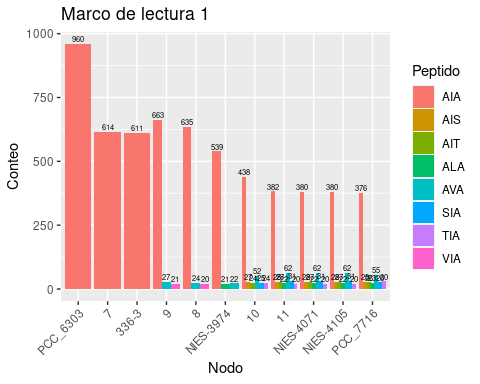
\includegraphics[width=1.1\linewidth]{ResultadosII_files/figure-latex/FIG58-1} 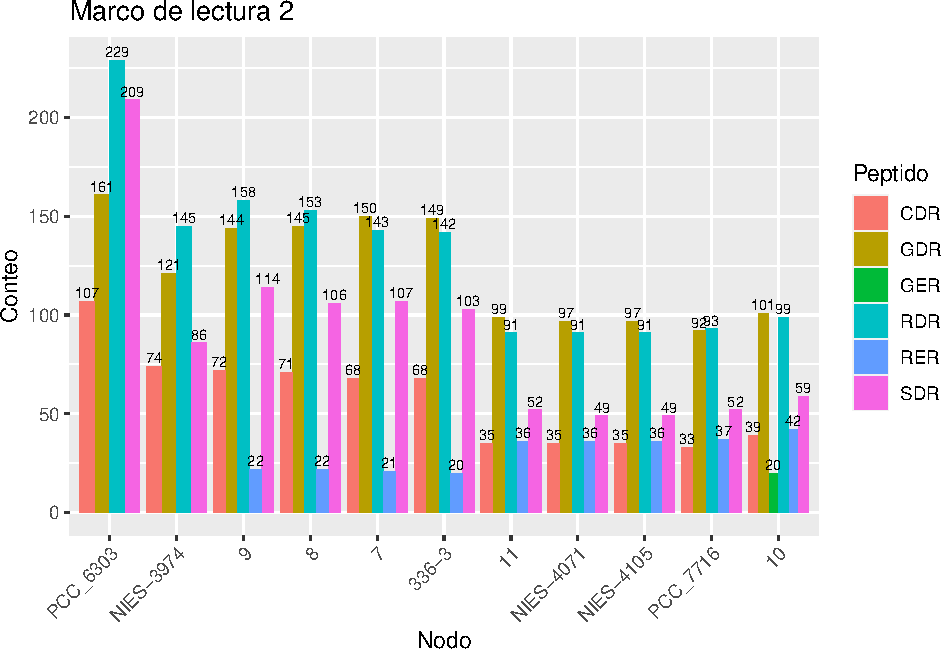
\includegraphics[width=1.1\linewidth]{ResultadosII_files/figure-latex/FIG58-2} 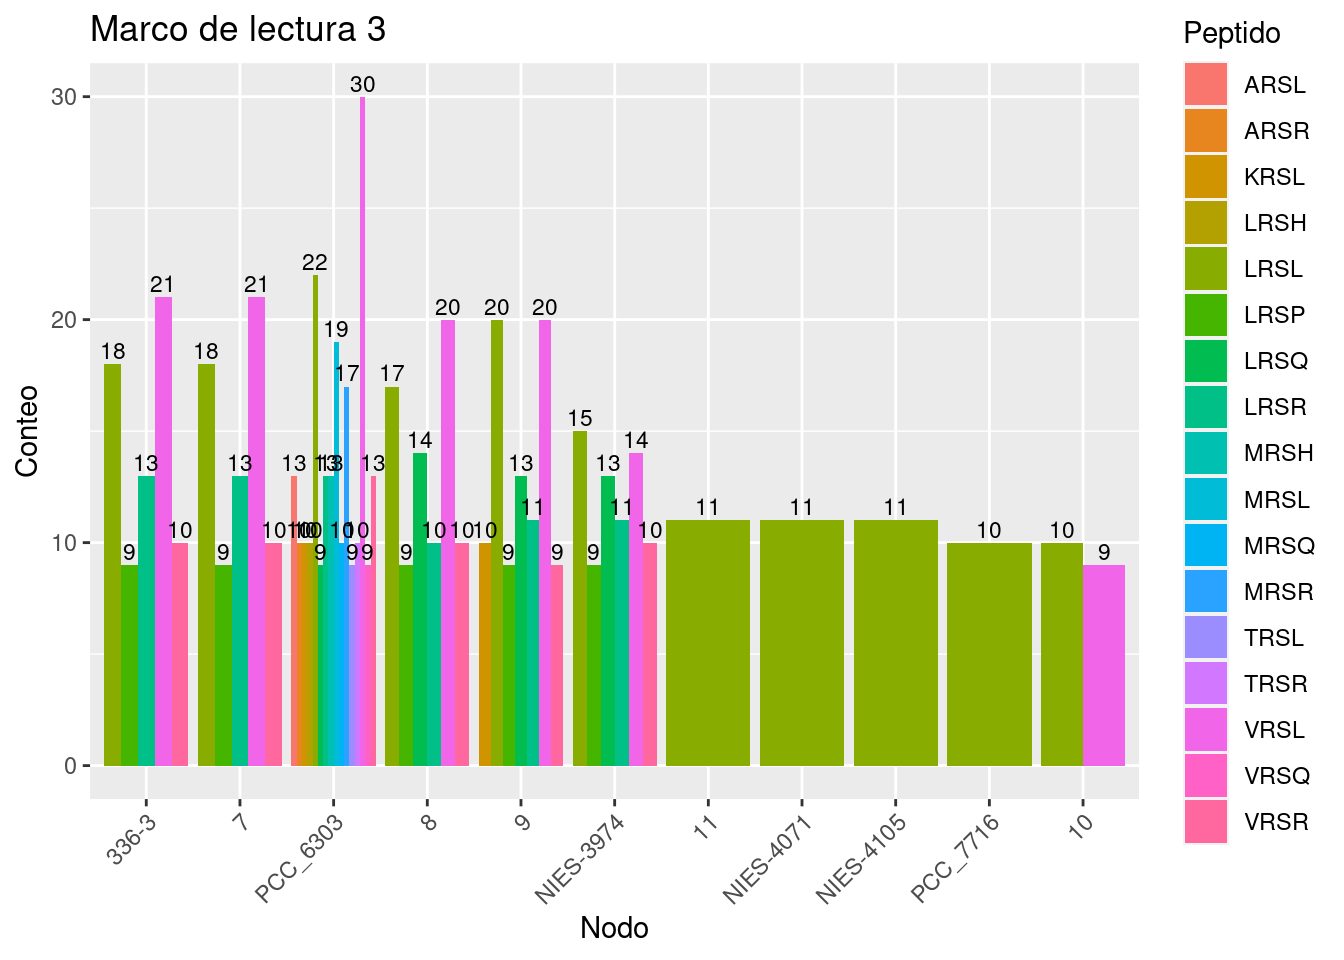
\includegraphics[width=1.1\linewidth]{ResultadosII_files/figure-latex/FIG58-3} 

}

\caption{**Abundancia de peptidos por cada nodo segun el marco de lectura.**.}\label{fig:FIG58}
\end{figure}

En la (Figura \ref{fig:FIG59}) mostramos 3 gráficos que indican la abundancia del tipo de mutaciones que hay en cada nodo de acuerdo al marco de lectura. Lo sitios de mutaciones mostrados pueden ser de los siguientes tipos:

\begin{itemize}
\tightlist
\item
  Conservative (la secuencia de AA cambió pero tiene similitud de acuerdo al score de BLOSUM62)
\item
  ConservativeNoSiteMut (la secuencia de AA cambió pero tiene similitud de acuerdo al score de BLOSUM62. Sin embargo, el sitio no sufrió mutaciones)
\item
  Deletion (La secuencia de AA tiene sufrio 1 o mas deleciones)
\item
  NoMutation (La secuencia de AA no sufrio mutaciones)
\item
  NoSynonym (La secuencia de AA cambió)
\item
  NoSynonymNoSiteMut (La secuencia de AA cambió. Sin embargo, el sitio no sufrió mutaciones.)
\item
  Synonym (El sitio sufrió mutaciones. Sin embargo, la secuencia de AA no cambió.)
\end{itemize}

\begin{figure}

{\centering 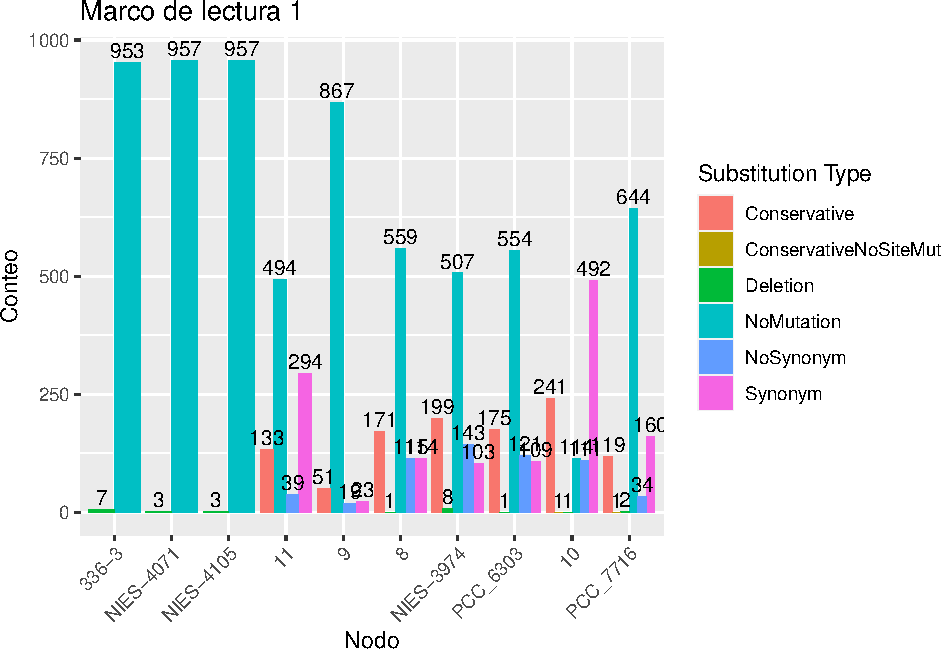
\includegraphics[width=1.1\linewidth]{ResultadosII_files/figure-latex/FIG59-1} 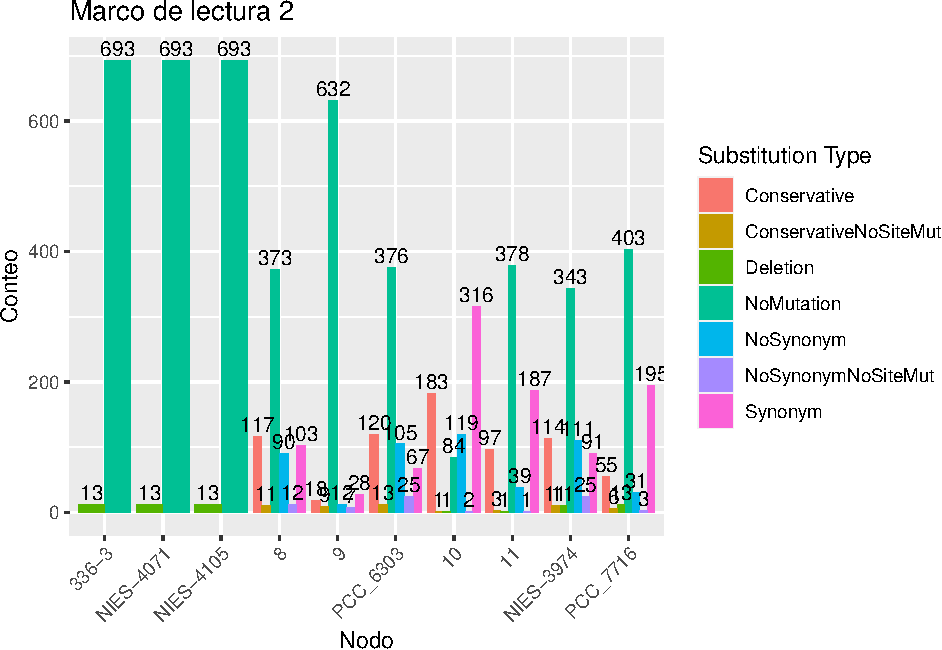
\includegraphics[width=1.1\linewidth]{ResultadosII_files/figure-latex/FIG59-2} 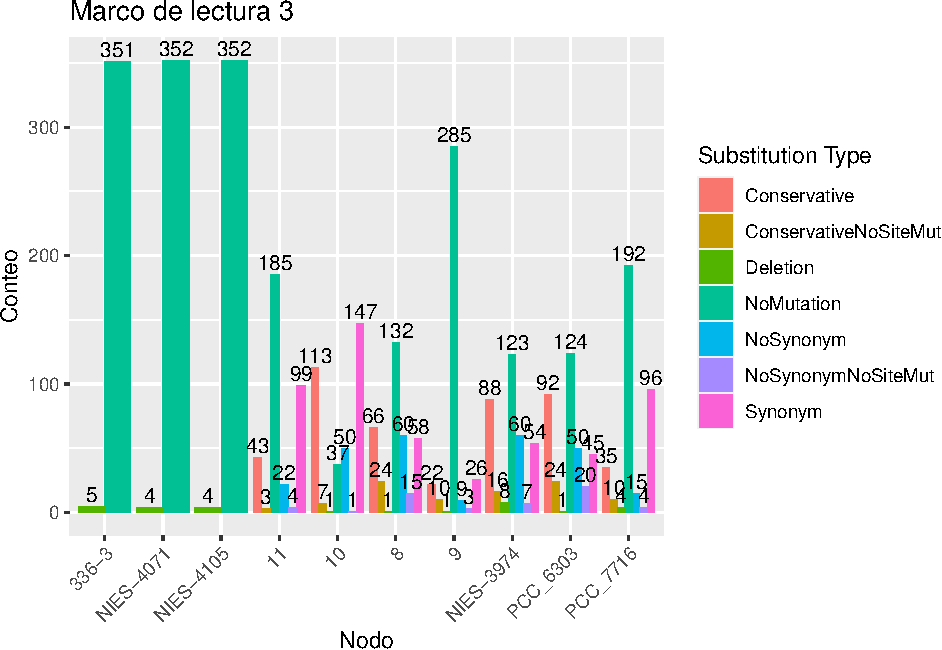
\includegraphics[width=1.1\linewidth]{ResultadosII_files/figure-latex/FIG59-3} 

}

\caption{**Abundancia del tipo de sustitución por cada nodo segun el marco de lectura.**.}\label{fig:FIG59}
\end{figure}

\hypertarget{anuxe1lisis-de-sitios-en-los-cuales-su-ancestro-era-hip1-2}{%
\subsubsection{Análisis de sitios en los cuales su ancestro era HIP1}\label{anuxe1lisis-de-sitios-en-los-cuales-su-ancestro-era-hip1-2}}

Para tratar de entender como es que los sitios HIP1 se pierden hicimos un análisis unicamente en en las transiciones en las que el nodo ancestral tenia un sitio HIP1.

En la (Figura \ref{fig:FIG60}) mostramos 3 gráficos que indican la frecuencia del tipo de sustituciones que hubo para estos casos para cada nodo en cada uno de los marcos de lectura.

\begin{figure}

{\centering \includegraphics[width=1.1\linewidth]{ResultadosII_files/figure-latex/FIG60-1} \includegraphics[width=1.1\linewidth]{ResultadosII_files/figure-latex/FIG60-2} \includegraphics[width=1.1\linewidth]{ResultadosII_files/figure-latex/FIG60-3} 

}

\caption{**Abundancia del tipo de sustitución por cada nodo segun el marco de lectura. Unicamente para transiciones en los que el nodo ancestral era un sitio HIP1.**}\label{fig:FIG60}
\end{figure}

En la (Figura \ref{fig:FIG61}) mostramos 3 gráficos (uno por cada marco de lectura) que indican la frecuencia de las mutaciones en cada uno de los 8 nucleótidos del sitio HIP.

\begin{figure}

{\centering \includegraphics[width=1.1\linewidth]{ResultadosII_files/figure-latex/FIG61-1} \includegraphics[width=1.1\linewidth]{ResultadosII_files/figure-latex/FIG61-2} \includegraphics[width=1.1\linewidth]{ResultadosII_files/figure-latex/FIG61-3} 

}

\caption{**Frecuencia de las mutaciones de cada nucleótido del sitio HIP para cada nodo segun el marco de lectura.**.}\label{fig:FIG61}
\end{figure}

En la (Figura \ref{fig:FIG62}) mostramos 3 gráficos (uno por cada marco de lectura) que indican la frecuencia del tipo sustitucion de bases.

\begin{figure}

{\centering \includegraphics[width=1.1\linewidth]{ResultadosII_files/figure-latex/FIG62-1} \includegraphics[width=1.1\linewidth]{ResultadosII_files/figure-latex/FIG62-2} \includegraphics[width=1.1\linewidth]{ResultadosII_files/figure-latex/FIG62-3} 

}

\caption{**Frecuencia del tipo de sustituciónes de base en los sitios HIP para cada marco de lectura**.}\label{fig:FIG62}
\end{figure}

\hypertarget{anuxe1lisis-de-sitios-en-los-cuales-solo-el-nodo-actual-tiene-hip1-2}{%
\subsubsection{Análisis de sitios en los cuales solo el nodo actual tiene HIP1}\label{anuxe1lisis-de-sitios-en-los-cuales-solo-el-nodo-actual-tiene-hip1-2}}

Para tratar de entender como es que los sitios HIP se ganan, hicimos un analisis unicamente en las transiciones en las que el nodo actual tenia un sitio HIP1.

En la Figura \ref{fig:FIG63} mostramos 3 gráficos (uno por cada marco de lectura) que indican la frecuencia del tipo de sustituciones que hubo para estos casos para cada nodo en cada uno de los marcos de lectura.

\begin{figure}

{\centering \includegraphics[width=1.1\linewidth]{ResultadosII_files/figure-latex/FIG63-1} \includegraphics[width=1.1\linewidth]{ResultadosII_files/figure-latex/FIG63-2} \includegraphics[width=1.1\linewidth]{ResultadosII_files/figure-latex/FIG63-3} 

}

\caption{**Abundancia del tipo de sustitución por cada nodo segun el marco de lectura. Unicamente para transiciones en los que el nodo actual era un sitio HIP1.**.}\label{fig:FIG63}
\end{figure}

\hypertarget{conjunto-de-sitios-hip1-unicos-en-las-especies-336-3-nies-3974-y-pcc_6303}{%
\subsection{Conjunto de sitios HIP1 unicos en las especies 336-3, NIES-3974 y PCC\_6303}\label{conjunto-de-sitios-hip1-unicos-en-las-especies-336-3-nies-3974-y-pcc_6303}}

\hypertarget{red-de-transiciones-3}{%
\subsubsection{Red de transiciones}\label{red-de-transiciones-3}}

Para aumentar el numero de ``experimentos'', buscamos todos los sitios HIP1 UNICOS existentes en el subclado que contiene a las especies 336-3, NIES-3974 y PCC\_6303.

Posteriormente creamos la red usando la función \texttt{Create\_Network()}:

y visualizamos dicha red .

Para visualizar la red usamos la paqueteria \texttt{networkD3}. Hicimos 2 figuras, la (Figura \ref{fig:FIG34}) muestra la red como una conexión de nodos a través de vertices con un grosor proporcional al numero de veces que ocurrió cada transición.

En la (Figura \ref{fig:FIG35}) podemos ver las transiciones de una forma mas ordenada, con el numero de ocurrencias y la dirección en la que ocurrieron.

\hypertarget{transiciones-entre-nodo-9-y-nodo-10-3}{%
\subsubsection{Transiciones entre Nodo 9 y Nodo 10}\label{transiciones-entre-nodo-9-y-nodo-10-3}}

En la (Figura \ref{fig:FIG36}) se muestra la red como una conexión de nodos a través de vertices con un grosor proporcional al numero de veces que ocurrió cada transición. En la (Figura \ref{fig:FIG37}) podemos ver las transiciones de una forma mas ordenada, con el numero de ocurrencias y la dirección en la que ocurrieron.

\hypertarget{mutaciones-en-los-codones-3}{%
\subsubsection{Mutaciones en los codones}\label{mutaciones-en-los-codones-3}}

Para entender como es que se van ganando o perdiendo los sitios palindrómicos hicimos un análisis del tipo mutaciones de los sitios. Esto lo hicimos viendo en que marco de lectura se encontraba cada nodo y revisando la secuencia de aminoacidos que codificaban. En la (Figura \ref{fig:FIG38}) mostramos 3 gráficos que indican la abundancia de los peptidos codificados por los sitios palindrómicos de acuerdo al marco de lectura en el que se encuentran. En esta figura podemos observar que el marco de lectura es el que contiene la mayoria de los sitios

\begin{figure}

{\centering \includegraphics[width=1.1\linewidth]{ResultadosII_files/figure-latex/FIG38-1} \includegraphics[width=1.1\linewidth]{ResultadosII_files/figure-latex/FIG38-2} \includegraphics[width=1.1\linewidth]{ResultadosII_files/figure-latex/FIG38-3} 

}

\caption{**Abundancia de peptidos por cada nodo segun el marco de lectura.**.}\label{fig:FIG38}
\end{figure}

En la (Figura \ref{fig:FIG39}) mostramos 3 gráficos que indican la abundancia del tipo de mutaciones que hay en cada nodo de acuerdo al marco de lectura. Lo sitios de mutaciones mostrados pueden ser de los siguientes tipos:

\begin{itemize}
\tightlist
\item
  Conservative (la secuencia de AA cambió pero tiene similitud de acuerdo al score de BLOSUM62)
\item
  ConservativeNoSiteMut (la secuencia de AA cambió pero tiene similitud de acuerdo al score de BLOSUM62. Sin embargo, el sitio no sufrió mutaciones)
\item
  Deletion (La secuencia de AA tiene sufrio 1 o mas deleciones)
\item
  NoMutation (La secuencia de AA no sufrio mutaciones)
\item
  NoSynonym (La secuencia de AA cambió)
\item
  NoSynonymNoSiteMut (La secuencia de AA cambió. Sin embargo, el sitio no sufrió mutaciones.)
\item
  Synonym (El sitio sufrió mutaciones. Sin embargo, la secuencia de AA no cambió.)
\end{itemize}

\begin{figure}

{\centering \includegraphics[width=1.1\linewidth]{ResultadosII_files/figure-latex/FIG39-1} \includegraphics[width=1.1\linewidth]{ResultadosII_files/figure-latex/FIG39-2} \includegraphics[width=1.1\linewidth]{ResultadosII_files/figure-latex/FIG39-3} 

}

\caption{**Abundancia del tipo de sustitución por cada nodo segun el marco de lectura.**.}\label{fig:FIG39}
\end{figure}

\hypertarget{anuxe1lisis-de-sitios-en-los-cuales-su-ancestro-era-hip1-3}{%
\subsubsection{Análisis de sitios en los cuales su ancestro era HIP1}\label{anuxe1lisis-de-sitios-en-los-cuales-su-ancestro-era-hip1-3}}

Para tratar de entender como es que los sitios HIP1 se pierden hicimos un análisis unicamente en en las transiciones en las que el nodo ancestral tenia un sitio HIP1.

En la (Figura \ref{fig:FIG40}) mostramos 3 gráficos que indican la frecuencia del tipo de sustituciones que hubo para estos casos para cada nodo en cada uno de los marcos de lectura.

\begin{figure}

{\centering \includegraphics[width=1.1\linewidth]{ResultadosII_files/figure-latex/FIG40-1} \includegraphics[width=1.1\linewidth]{ResultadosII_files/figure-latex/FIG40-2} \includegraphics[width=1.1\linewidth]{ResultadosII_files/figure-latex/FIG40-3} 

}

\caption{**Abundancia del tipo de sustitución por cada nodo segun el marco de lectura. Unicamente para transiciones en los que el nodo ancestral era un sitio HIP1.**}\label{fig:FIG40}
\end{figure}

En la (Figura \ref{fig:FIG41}) mostramos 3 gráficos (uno por cada marco de lectura) que indican la frecuencia de las mutaciones en cada uno de los 8 nucleótidos del sitio HIP.

\begin{figure}

{\centering \includegraphics[width=1.1\linewidth]{ResultadosII_files/figure-latex/FIG41-1} \includegraphics[width=1.1\linewidth]{ResultadosII_files/figure-latex/FIG41-2} \includegraphics[width=1.1\linewidth]{ResultadosII_files/figure-latex/FIG41-3} 

}

\caption{**Frecuencia de las mutaciones de cada nucleótido del sitio HIP para cada nodo segun el marco de lectura.**.}\label{fig:FIG41}
\end{figure}

En la (Figura \ref{fig:FIG42}) mostramos 3 gráficos (uno por cada marco de lectura) que indican la frecuencia del tipo sustitucion de bases.

\begin{figure}

{\centering \includegraphics[width=1.1\linewidth]{ResultadosII_files/figure-latex/FIG42-1} \includegraphics[width=1.1\linewidth]{ResultadosII_files/figure-latex/FIG42-2} \includegraphics[width=1.1\linewidth]{ResultadosII_files/figure-latex/FIG42-3} 

}

\caption{**Frecuencia del tipo de sustituciónes de base en los sitios HIP para cada marco de lectura**.}\label{fig:FIG42}
\end{figure}

\hypertarget{anuxe1lisis-de-sitios-en-los-cuales-solo-el-nodo-actual-tiene-hip1-3}{%
\subsubsection{Análisis de sitios en los cuales solo el nodo actual tiene HIP1}\label{anuxe1lisis-de-sitios-en-los-cuales-solo-el-nodo-actual-tiene-hip1-3}}

Para tratar de entender como es que los sitios HIP se ganan, hicimos un analisis unicamente en las transiciones en las que el nodo actual tenia un sitio HIP1.

En la Figura \ref{fig:FIG43} mostramos 3 gráficos (uno por cada marco de lectura) que indican la frecuencia del tipo de sustituciones que hubo para estos casos para cada nodo en cada uno de los marcos de lectura.

\begin{figure}

{\centering \includegraphics[width=1.1\linewidth]{ResultadosII_files/figure-latex/FIG43-1} \includegraphics[width=1.1\linewidth]{ResultadosII_files/figure-latex/FIG43-2} \includegraphics[width=1.1\linewidth]{ResultadosII_files/figure-latex/FIG43-3} 

}

\caption{**Abundancia del tipo de sustitución por cada nodo segun el marco de lectura. Unicamente para transiciones en los que el nodo actual era un sitio HIP1.**.}\label{fig:FIG43}
\end{figure}

\hypertarget{tggcgcca}{%
\subsection{TGGCGCCA}\label{tggcgcca}}

\hypertarget{red-de-transiciones-4}{%
\subsubsection{Red de transiciones}\label{red-de-transiciones-4}}

Para hacer mas visual la reconstrucción, construimos una red de las transiciones entre los estados ancestrales. Esto lo hicimos en r usando la función \texttt{Create\_Transition\_Table()}:

\begin{Shaded}
\begin{Highlighting}[]
\FunctionTok{source}\NormalTok{(}\StringTok{"ASR\_Orth\_Functions/NodeAndEdges.R"}\NormalTok{)}
\NormalTok{Nodes.Edges }\OtherTok{\textless{}{-}} \FunctionTok{Create\_Transition\_Table}\NormalTok{(}\AttributeTok{SitesTable =} \StringTok{"Clados/Callothrix\_clade/PALINDROMES/TGGCGCCA/PCC\_7716/Orthologues\_Palindrome\_sites.txt"}\NormalTok{,}
                                \AttributeTok{EvolutionModel =} \StringTok{"F81"}\NormalTok{,}
                                \AttributeTok{Method =} \StringTok{"bayes"}\NormalTok{,}
                                \AttributeTok{Phylogeny =} \StringTok{"Clados/Callothrix\_clade/SpeciesTree\_rooted.txt"}\NormalTok{,}
                                \AttributeTok{OrthoPath =} \StringTok{"Clados/Callothrix\_clade/PALINDROMES/TGGCGCCA/PCC\_7716/Only\_ORTHOLOGUES/"}\NormalTok{)}
\end{Highlighting}
\end{Shaded}

Posteriormente creamos la red usando la función \texttt{Create\_Network()}:

y visualizamos dicha red .

Para visualizar la red usamos la paqueteria \texttt{networkD3}. Hicimos 2 figuras, la (Figura \ref{fig:FIG24}) muestra la red como una conexión de nodos a través de vertices con un grosor proporcional al numero de veces que ocurrió cada transición. En dicha red podemos ver algunos nodos con bordes muy gruesos como \textbf{GCAATTGC}, \textbf{GCAATCGC}, \textbf{GCAATAGC}, \textbf{GCGATTGC} (Tabla \ref{tab:TAB62}).

En la (Figura \ref{fig:FIG25}) podemos ver las transiciones de una forma mas ordenada, con el numero de ocurrencias y la dirección en la que ocurrieron.

\hypertarget{transiciones-entre-nodo-9-y-nodo-10-4}{%
\subsubsection{Transiciones entre Nodo 9 y Nodo 10}\label{transiciones-entre-nodo-9-y-nodo-10-4}}

Para entender más como es que se gana o se pierden los sitios palindrómicos revisamos la transición en tre los nodos 9 y 10. Esto es porque es esta transicion de nodos la que separa a los dos subclados entre los que hay una repentino cambio de abundancia de sitios palindrómicos (Figura \ref{fig:FIG15}).

Para hacer esto filtramos los datos de la red para mostrar unicamente las transiciones que se dieron entre los nodos 9 y 10 e hicimos las mismas figuras.
En la (Figura \ref{fig:FIG26}) se muestra la red como una conexión de nodos a través de vertices con un grosor proporcional al numero de veces que ocurrió cada transición. En la (Figura \ref{fig:FIG27}) podemos ver las transiciones de una forma mas ordenada, con el numero de ocurrencias y la dirección en la que ocurrieron.

\hypertarget{mutaciones-en-los-codones-4}{%
\subsubsection{Mutaciones en los codones}\label{mutaciones-en-los-codones-4}}

Para entender como es que se van ganando o perdiendo los sitios palindrómicos hicimos un análisis del tipo mutaciones de los sitios. Esto lo hicimos viendo en que marco de lectura se encontraba cada nodo y revisando la secuencia de aminoacidos que codificaban. En la (Figura \ref{fig:FIG28}) mostramos 3 gráficos que indican la abundancia de los peptidos codificados por los sitios palindrómicos de acuerdo al marco de lectura en el que se encuentran.

\begin{figure}

{\centering \includegraphics[width=1.1\linewidth]{ResultadosII_files/figure-latex/FIG28-1} \includegraphics[width=1.1\linewidth]{ResultadosII_files/figure-latex/FIG28-2} \includegraphics[width=1.1\linewidth]{ResultadosII_files/figure-latex/FIG28-3} 

}

\caption{**Abundancia de peptidos por cada nodo segun el marco de lectura.**.}\label{fig:FIG28}
\end{figure}

En la (Figura \ref{fig:FIG29}) mostramos 3 gráficos que indican la abundancia del tipo de mutaciones que hay en cada nodo de acuerdo al marco de lectura. Lo sitios de mutaciones mostrados pueden ser de los siguientes tipos:

\begin{itemize}
\tightlist
\item
  Conservative (la secuencia de AA cambió pero tiene similitud de acuerdo al score de BLOSUM62)
\item
  ConservativeNoSiteMut (la secuencia de AA cambió pero tiene similitud de acuerdo al score de BLOSUM62. Sin embargo, el sitio no sufrió mutaciones)
\item
  Deletion (La secuencia de AA tiene sufrio 1 o mas deleciones)
\item
  NoMutation (La secuencia de AA no sufrio mutaciones)
\item
  NoSynonym (La secuencia de AA cambió)
\item
  NoSynonymNoSiteMut (La secuencia de AA cambió. Sin embargo, el sitio no sufrió mutaciones.)
\item
  Synonym (El sitio sufrió mutaciones. Sin embargo, la secuencia de AA no cambió.)
\end{itemize}

\begin{figure}

{\centering \includegraphics[width=1.1\linewidth]{ResultadosII_files/figure-latex/FIG29-1} \includegraphics[width=1.1\linewidth]{ResultadosII_files/figure-latex/FIG29-2} \includegraphics[width=1.1\linewidth]{ResultadosII_files/figure-latex/FIG29-3} 

}

\caption{**Abundancia del tipo de sustitución por cada nodo segun el marco de lectura.**.}\label{fig:FIG29}
\end{figure}

\hypertarget{anuxe1lisis-de-sitios-en-los-cuales-su-ancestro-era-tggcgcca}{%
\subsubsection{Análisis de sitios en los cuales su ancestro era TGGCGCCA}\label{anuxe1lisis-de-sitios-en-los-cuales-su-ancestro-era-tggcgcca}}

Para tratar de entender como es que los sitios HIP1 se pierden hicimos un análisis unicamente en en las transiciones en las que el nodo ancestral tenia un sitio TGGCGCCA.

En la (Figura \ref{fig:FIG30}) mostramos 3 gráficos que indican la frecuencia del tipo de sustituciones que hubo para estos casos para cada nodo en cada uno de los marcos de lectura.

En la (Figura \ref{fig:FIG31}) mostramos 3 gráficos (uno por cada marco de lectura) que indican la frecuencia de las mutaciones en cada uno de los 8 nucleótidos del sitio HIP.

En la (Figura \ref{fig:FIG32}) mostramos 3 gráficos (uno por cada marco de lectura) que indican la frecuencia del tipo sustitucion de bases.

\begin{figure}

{\centering \includegraphics[width=1.1\linewidth]{ResultadosII_files/figure-latex/FIG30-1} \includegraphics[width=1.1\linewidth]{ResultadosII_files/figure-latex/FIG30-2} \includegraphics[width=1.1\linewidth]{ResultadosII_files/figure-latex/FIG30-3} 

}

\caption{**Abundancia del tipo de sustitución por cada nodo segun el marco de lectura. Unicamente para transiciones en los que el nodo ancestral era un sitio TGGCGCCA.**}\label{fig:FIG30}
\end{figure}

\begin{figure}

{\centering \includegraphics[width=1.1\linewidth]{ResultadosII_files/figure-latex/FIG31-1} \includegraphics[width=1.1\linewidth]{ResultadosII_files/figure-latex/FIG31-2} \includegraphics[width=1.1\linewidth]{ResultadosII_files/figure-latex/FIG31-3} 

}

\caption{**Frecuencia de las mutaciones de cada nucleótido del sitio TGGCGCCA para cada nodo segun el marco de lectura.**.}\label{fig:FIG31}
\end{figure}

\begin{figure}

{\centering \includegraphics[width=1.1\linewidth]{ResultadosII_files/figure-latex/FIG32-1} \includegraphics[width=1.1\linewidth]{ResultadosII_files/figure-latex/FIG32-2} \includegraphics[width=1.1\linewidth]{ResultadosII_files/figure-latex/FIG32-3} 

}

\caption{**Frecuencia del tipo de sustituciónes de base en los sitios TGGCGCCA para cada marco de lectura**.}\label{fig:FIG32}
\end{figure}

\hypertarget{anuxe1lisis-de-sitios-en-los-cuales-solo-el-nodo-actual-tiene-tggcgcca}{%
\subsubsection{Análisis de sitios en los cuales solo el nodo actual tiene TGGCGCCA}\label{anuxe1lisis-de-sitios-en-los-cuales-solo-el-nodo-actual-tiene-tggcgcca}}

Para tratar de entender como es que los sitios TGGCGCCA se ganan, hicimos un analisis unicamente en las transiciones en las que el nodo actual tenia un sitio TGGCGCCA.

En la Figura \ref{fig:FIG33} mostramos 3 gráficos (uno por cada marco de lectura) que indican la frecuencia del tipo de sustituciones que hubo para estos casos para cada nodo en cada uno de los marcos de lectura.

\begin{figure}

{\centering \includegraphics[width=1.1\linewidth]{ResultadosII_files/figure-latex/FIG33-1} \includegraphics[width=1.1\linewidth]{ResultadosII_files/figure-latex/FIG33-2} \includegraphics[width=1.1\linewidth]{ResultadosII_files/figure-latex/FIG33-3} 

}

\caption{**Abundancia del tipo de sustitución por cada nodo segun el marco de lectura. Unicamente para transiciones en los que el nodo actual era un sitio TGGCGCCA.**.}\label{fig:FIG33}
\end{figure}

  \bibliography{book.bib,packages.bib}

\end{document}
